% Seminar: Ipoteza Pieței Eficiente (EMH) --- Versiune completă
% Statistica Piețelor Financiare --- combină seminar_emh_ro.tex (grafice + scenarii)
% cu seminar_emh_ipoteza_pietei_eficiente_ro.tex (exerciții manuale + Python + BVB)

\documentclass[9pt, aspectratio=169, t]{beamer}
%=============================================================================
% PREAMBUL COMUN - Statistica Piețelor Financiare
% Versiune robustă pentru macOS (MacTeX / BasicTeX / TeX Live)
% Daniel Traian Pele, Antoaneta Amza - ASE București
%
% MODIFICĂRI față de varianta originală:
%  (1) fontawesome5 făcut OPȚIONAL (\IfFileExists) → nu mai pică dacă lipsește
%  (2) polyglossia cu fallback automat pe babel dacă romanian nu există
%  (3) setmainfont rescris cu Ligatures=TeX și nume normalizate (merge pe macOS)
%  (4) graphicspath extins (include directorul curent + variante relative) ca
%      logo-urile să fie găsite și când lansezi xelatex dintr-un subdirector
%
% Compilare:  xelatex preamble + main, de DOUĂ ori (toc/ref).
%=============================================================================

% Asigură încadrarea conținutului pe diapozitive
\setbeamersize{text margin left=8mm, text margin right=8mm}

%=============================================================================
% CONFIGURARE TEMĂ ȘI STIL
%=============================================================================
\usetheme{default}

% Paletă de Culori
\definecolor{MainBlue}{RGB}{26, 58, 110}
\definecolor{AccentBlue}{RGB}{26, 58, 110}
\definecolor{IDAred}{RGB}{205, 0, 0}
\definecolor{DarkGray}{RGB}{51, 51, 51}
\definecolor{MediumGray}{RGB}{128, 128, 128}
\definecolor{LightGray}{RGB}{248, 248, 248}
\definecolor{VeryLightGray}{RGB}{235, 235, 235}
\definecolor{KeynoteGray}{RGB}{218, 218, 218}
\definecolor{SectionGray}{RGB}{120, 120, 120}
\definecolor{FooterGray}{RGB}{100, 100, 100}
\definecolor{Crimson}{RGB}{220, 53, 69}
\definecolor{Forest}{RGB}{46, 125, 50}
\definecolor{Amber}{RGB}{181, 133, 63}
\definecolor{Orange}{RGB}{230, 126, 34}
\definecolor{Purple}{RGB}{142, 68, 173}

% Fundal gradient (gradient Keynote exact 315°: alb la RGB 218,218,218)
\setbeamertemplate{background}{%
	\begin{tikzpicture}[remember picture, overlay]
		\shade[shading=axis, shading angle=315,
		top color=white, bottom color=KeynoteGray]
		(current page.south west) rectangle (current page.north east);
	\end{tikzpicture}%
}
% Culoare solidă de rezervă pentru compatibilitate
\setbeamercolor{background canvas}{bg=}

\setbeamercolor{palette primary}{bg=MainBlue, fg=white}
\setbeamercolor{palette secondary}{bg=MainBlue!85, fg=white}
\setbeamercolor{palette tertiary}{bg=MainBlue!70, fg=white}
\setbeamercolor{structure}{fg=MainBlue}
\setbeamercolor{title}{fg=IDAred}
\setbeamercolor{frametitle}{fg=IDAred, bg=}
\setbeamercolor{block title}{bg=MainBlue, fg=white}
\setbeamercolor{block body}{bg=VeryLightGray, fg=DarkGray}
\setbeamercolor{block title alerted}{bg=Crimson, fg=white}
\setbeamercolor{block body alerted}{bg=Crimson!8, fg=DarkGray}
\setbeamercolor{block title example}{bg=Forest, fg=white}
\setbeamercolor{block body example}{bg=Forest!8, fg=DarkGray}
\setbeamercolor{item}{fg=MainBlue}

\setbeamerfont{institute}{size=\footnotesize}

\setbeamercolor{author in head/foot}{fg=FooterGray, bg=}
\setbeamercolor{title in head/foot}{fg=FooterGray, bg=}
\setbeamercolor{date in head/foot}{fg=FooterGray, bg=}
\setbeamercolor{section in head/foot}{fg=FooterGray, bg=}
\setbeamercolor{subsection in head/foot}{fg=FooterGray, bg=}

\setbeamertemplate{itemize item}{\color{MainBlue}$\boxdot$}
\setbeamertemplate{itemize subitem}{\color{MainBlue}$\blacktriangleright$}
\setbeamertemplate{itemize subsubitem}{\color{MainBlue}\tiny$\bullet$}
\setbeamertemplate{itemize/enumerate body begin}{\normalsize}
\setbeamertemplate{itemize/enumerate subbody begin}{\normalsize}

\setbeamertemplate{section in toc}{%
	\leavevmode\leftskip=1.5em%
	\llap{\color{MainBlue}$\boxdot$\kern0.5em}%
	\inserttocsection\par%
}

\setlength{\leftmargini}{10pt}
\setlength{\leftmarginii}{10pt}
\makeatletter
\def\@listi{\leftmargin\leftmargini \topsep 0pt \parsep 0pt \itemsep 0pt}
\def\@listii{\leftmargin\leftmarginii \topsep 0pt \parsep 0pt \itemsep 0pt}
\makeatother

\setbeamertemplate{navigation symbols}{}

%=============================================================================
% ANTET PERSONALIZAT
%=============================================================================
\setbeamertemplate{headline}{%
	\vskip10pt%
	\hbox to \paperwidth{%
		\hskip0.5cm%
		{\small\color{FooterGray}\renewcommand{\hyperlink}[2]{##2}\insertsectionhead}%
		\hfill%
		\textcolor{FooterGray}{\small\insertframenumber}%
		\hskip0.5cm%
	}%
	\vskip4pt%
	{\color{FooterGray}\hrule height 0.4pt}%
}

%=============================================================================
% PACHETE — ordine importantă: fontspec ÎNAINTE de polyglossia/babel
%=============================================================================

% --- (1) FONTSPEC + FONTURI ROBUSTE PE macOS ---
\usepackage{fontspec}
% Pe macOS unele fonturi Latin Modern nu sunt înregistrate ca fonturi de sistem.
% Folosim Ligatures=TeX (pentru -- → en-dash etc.) și lăsăm fontspec să caute
% prin kpathsea (merge atât pe Mac, cât și pe Linux/Windows).
\defaultfontfeatures{Ligatures=TeX}
\IfFontExistsTF{Latin Modern Roman}{%
	\setmainfont{Latin Modern Roman}
	\setsansfont{Latin Modern Sans}
	\setmonofont{Latin Modern Mono}
}{%
	% Fallback dacă numele cu spații nu sunt găsite (cazul macOS fără fonturi
	% Latin Modern în /Library/Fonts) — fontspec va folosi fontul implicit.
	\PackageWarning{preamble}{Latin Modern Roman nu a fost gasit; folosesc fontul implicit.}
}

% --- (2) POLYGLOSSIA SAU BABEL CU FALLBACK ---
% Pe versiuni vechi de polyglossia (TeX Live < 2020) limba `romanian` nu există.
% Detectăm și folosim babel ca rezervă.
\IfFileExists{gloss-romanian.ldf}{%
	\usepackage{polyglossia}
	\setdefaultlanguage{romanian}
	\setotherlanguage{english}
}{%
	\PackageWarning{preamble}{polyglossia/romanian indisponibil; folosesc babel.}
	\usepackage[english,romanian]{babel}
}

% --- (3) MATH ȘI GRAFICĂ ---
\usepackage{amsmath, amssymb, amsthm}
\usepackage{mathtools}
\usepackage{bm}
\usepackage{tikz}
\usetikzlibrary{arrows.meta, positioning, shapes, calc, decorations.pathreplacing, shadings}
\usepackage{booktabs}
\usepackage{multirow}
\usepackage{array}
\usepackage{graphicx}
\usepackage{hyperref}
\usepackage{colortbl}
\usepackage{listings}
\lstset{basicstyle=\ttfamily\small, breaklines=true, frame=single, backgroundcolor=\color{VeryLightGray}}
\hypersetup{colorlinks=true, linkcolor=MainBlue, urlcolor=MainBlue}

% --- (4) GRAPHICSPATH cu directorul curent inclus ca fallback ---
\graphicspath{{./}{./logos/}{./charts/}{./photos/}{../logos/}{../charts/}{../photos/}{../../logos/}{../../charts/}{../../photos/}}
\hfuzz=2pt
\vfuzz=2pt

%=============================================================================
% SUBSOL PERSONALIZAT — fontawesome5 făcut OPȚIONAL
%=============================================================================
% Pe BasicTeX / instalări minime de MacTeX, fontawesome5 nu există.
% Dacă lipsește, omitem icoanele (subsolul rămâne curat).
\IfFileExists{fontawesome5.sty}{%
	\usepackage{fontawesome5}
	\newcommand{\hasfontawesome}{true}
}{%
	\PackageWarning{preamble}{fontawesome5 indisponibil; subsolul nu va contine icoane.}
}

\setbeamertemplate{footline}{%
	{\color{FooterGray}\hrule height 0.4pt}%
	\vskip4pt%
	\hbox to \paperwidth{%
		\hskip0.5cm%
		\textcolor{FooterGray}{\small Statistica Piețelor Financiare}%
		\hfill%
		\raisebox{-0.1em}{%
			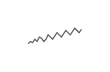
\begin{tikzpicture}[x=0.08em, y=0.08em, line width=0.4pt]
				\draw[FooterGray] (0,3) -- (1,4) -- (2,3.5) -- (3,5) -- (4,4) -- (5,6) -- (6,5.5) -- (7,4) -- (8,5) -- (9,7) -- (10,6) -- (11,5) -- (12,6.5) -- (13,8) -- (14,7) -- (15,6) -- (16,7.5) -- (17,9) -- (18,8) -- (19,7) -- (20,8.5) -- (21,10) -- (22,9) -- (23,8) -- (24,9.5);
			\end{tikzpicture}%
		}%
		\hskip0.5cm%
	}%
	\vskip6pt%
}

%=============================================================================
% COMANDA QUANTLET
%=============================================================================
\newcommand{\quantlet}[2]{%
	\hfill\href{#2}{%
		\raisebox{-0.15em}{
\includegraphics[height=0.7em]{ql_logo.png}}%
		\textcolor{MainBlue}{\tiny\ #1}%
	}%
}

%=============================================================================
% PAGINĂ TITLU PERSONALIZATĂ
%=============================================================================
\defbeamertemplate*{title page}{hybrid}[1][]
{
	\vspace{0.2cm}
	\noindent\makebox[\linewidth][s]{%
		\href{https://www.ase.ro}{
\includegraphics[height=1.0cm]{ase_logo.png}}\hfill%
		\href{https://theida.net}{
\includegraphics[height=1.0cm]{ida_logo.png}}\hfill%
		\href{https://blockchain-research-center.com}{
\includegraphics[height=1.0cm]{brc_logo.png}}\hfill%
		\href{https://www.ai4efin.ase.ro}{
\includegraphics[height=1.0cm]{ai4efin_logo.png}}\hfill%
		\href{https://ipe.ro/new}{
\includegraphics[height=1.0cm]{acad_logo.png}}\hfill%
		\href{https://www.digital-finance-msca.com}{
\includegraphics[height=1.0cm]{msca_logo.png}}%
	}
	\vspace{0.6cm}
	
	\noindent\makebox[\linewidth][c]{%
		\begin{minipage}{0.11\linewidth}
			\centering
			\href{https://quantlet.com}{
\includegraphics[height=1.1cm]{ql_logo.png}}
		\end{minipage}%
		\begin{minipage}{0.76\linewidth}
			\centering
			{\LARGE\bfseries\usebeamercolor[fg]{title}\inserttitle}
			
			\vspace{0.3cm}
			
			{\usebeamerfont{subtitle}\usebeamercolor[fg]{title}\insertsubtitle}
		\end{minipage}%
		\begin{minipage}{0.11\linewidth}
			\centering
			\href{https://quantinar.com}{
\includegraphics[height=1.1cm]{qr_logo.png}}
		\end{minipage}%
	}
	
	\vspace{0.6cm}
	
	\hspace{0.5cm}{\usebeamerfont{author}\insertauthor}
	
	\vspace{0.3cm}
	
	\hspace{0.5cm}\begin{minipage}[t]{0.9\textwidth}
		\raggedright\small\insertinstitute
	\end{minipage}
}
\setbeamertemplate{title page}[hybrid]

%=============================================================================
% MEDII PENTRU TEOREME
%=============================================================================
\theoremstyle{definition}
\setbeamertemplate{theorems}[numbered]
\newtheorem{defn}{Definiție}
\newtheorem{thm}{Teoremă}
\newtheorem{prop}{Propoziție}
\newtheorem{rmk}{Observație}

%=============================================================================
% CENTRED MINIPAGE
%=============================================================================
\newenvironment{cminipage}[1]{%
	\par\noindent\hfill\begin{minipage}{#1}\ignorespaces
	}{%
	\end{minipage}\hfill\null\par
}

%=============================================================================
% COMENZI PERSONALIZATE
%=============================================================================
\newcommand{\E}{\mathbb{E}}
\newcommand{\Var}{\text{Var}}
\newcommand{\Cov}{\text{Cov}}
\newcommand{\Corr}{\text{Corr}}
\newcommand{\VaR}{\text{VaR}}
\newcommand{\ES}{\text{ES}}
\newcommand{\R}{\mathbb{R}}
\newcommand{\N}{\mathbb{N}}
\newcommand{\Z}{\mathbb{Z}}
\newcommand{\B}{\mathbf{B}}
\newcommand{\imark}{\textcolor{MainBlue}{\textbullet}}
\newcommand{\RMSE}{\text{RMSE}}
\newcommand{\MAE}{\text{MAE}}
\newcommand{\MAPE}{\text{MAPE}}
\newcommand{\correct}{\textcolor{Forest}{\checkmark}}
\newcommand{\incorrect}{\textcolor{Crimson}{\texttimes}}

%=============================================================================
% INFORMAȚII TITLU
%=============================================================================
\title[Statistica Piețelor Financiare]{Statistica Piețelor Financiare}
\author[D.T. Pele, A. Amza]{\texorpdfstring{\begin{tabular}[t]{@{}l@{}}Daniel Traian PELE \\ Antoaneta Amza\end{tabular}}{Daniel Traian PELE, Antoaneta Amza}}
\institute{Academia de Studii Economice din București\\
	IDA Institute Digital Assets\\
	Blockchain Research Center\\
	AI4EFin Artificial Intelligence for Energy Finance\\
	Academia Română, Institutul de Prognoză Economică\\
	MSCA Digital Finance}
\date{}
\subtitle{Seminar: Ipoteza Pieței Eficiente}

\begin{document}

% Colab base URL pentru quantlets Ch_04
\newcommand{\ch}[1]{\href{https://colab.research.google.com/github/QuantLet/Stat_fin_markets/blob/master/Ch_04/SFM_ch4_#1/SFM_ch4_#1.ipynb}{#1}}

%=============================================================================
% TITLU
%=============================================================================
{
\setbeamertemplate{headline}{}
\setbeamertemplate{footline}{}
\begin{frame}
    \titlepage
\end{frame}
}

%=============================================================================
% CUPRINS
%=============================================================================
\begin{frame}[shrink=15]{Cuprins (Contents)}
\begin{cminipage}{0.95\textwidth}
\begin{itemize}\setlength{\itemsep}{0pt}
    \item \textbf{Partea I: Teorie EMH} --- Cele 3 forme (Fama, 1970), random walk, martingal
    \item \textbf{Partea II: Autocorelație și Ljung--Box} --- ACF, formule, S\&P 500, randamente vs $r_t^2$, BVB
    \item \textbf{Partea III: Runs test} --- Secvențe de semne, statistica $Z$
    \item \textbf{Partea IV: Variance Ratio} --- VR(q), exercițiu manual, profil multi-piață, IC 95\%
    \item \textbf{Partea V: Cozi grele și limitele testelor} --- Normal vs Cauchy, McCulloch, robustețe
    \item \textbf{Partea VI: Event Study (semi-tare)} --- AR, CAR, scenarii, IC 95\%, grid AAPL, exercițiu manual
    \item \textbf{Partea VII: AMH și anomalii} --- Eficiență variabilă în timp, calendar, AMH (Lo, 2004)
    \item \textbf{Partea VIII: Strategii, costuri și SPIVA} --- MA crossover, pre/post 1990, active vs passive, bule
    \item \textbf{Partea IX: Studii de caz} --- Cross-asset, BVB, crypto, FX, sub-perioade, bootstrap CI
    \item \textbf{Partea X: AI checks și discuții} --- Verificarea codului LLM, scenarii practice
    \item \textbf{Partea XI: Studiu de caz S\&P 500 + temă BVB} --- Pipeline complet pe S\&P 500, aplicație practică pe date românești
    \item \textbf{Partea XII: Quiz și concluzii} --- Adevărat/Fals, întrebări cu răspunsuri, bibliografie
\end{itemize}
\end{cminipage}
\end{frame}

%=============================================================================
% OBIECTIVE
%=============================================================================
\section{Obiective}

\begin{frame}[shrink=15]{Obiective de învățare (Learning Objectives)}
\begin{cminipage}{0.95\textwidth}
\begin{columns}[T]
\begin{column}{0.55\textwidth}
\begin{block}{La finalul seminarului veți putea:}
\begin{itemize}\setlength{\itemsep}{0pt}
    \item Defini EMH și distinge formele
    \begin{itemize}\setlength{\itemsep}{0pt}
        \item Slabă (weak), semi-tare (semi-strong), tare (strong)
    \end{itemize}
    \item Verifica proprietatea de martingal a unui random walk
    \item Calcula manual autocorelația, $Q$ Ljung--Box, runs, $VR$
    \item Realiza un event study complet (AR, CAR, test $t$)
    \item Interpreta intervalele de încredere pentru $VR$ și CAR
    \item Înțelege Adaptive Markets Hypothesis (Lo, 2004)
    \item Înțelege de ce strategiile active subperformează (SPIVA)
    \item Compara eficiența pe diferite piețe (BVB, crypto, dezvoltate)
\end{itemize}
\end{block}
\end{column}
\begin{column}{0.42\textwidth}
\begin{center}
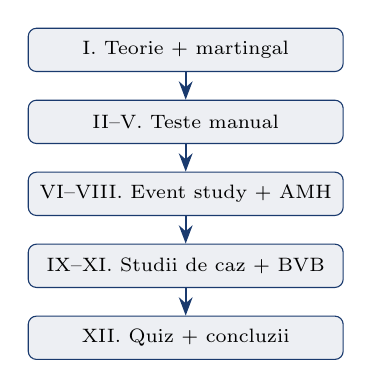
\begin{tikzpicture}[
    node distance=0.35cm,
    every node/.style={font=\scriptsize, align=center},
    phase/.style={draw=MainBlue, fill=MainBlue!8, rounded corners=3pt,
                  minimum width=4.0cm, minimum height=0.55cm}
]
\node[phase] (p1) {I. Teorie + martingal};
\node[phase, below=of p1] (p2) {II--V. Teste manual};
\node[phase, below=of p2] (p3) {VI--VIII. Event study + AMH};
\node[phase, below=of p3] (p4) {IX--XI. Studii de caz + BVB};
\node[phase, below=of p4] (p5) {XII. Quiz + concluzii};
\draw[-{Stealth}, MainBlue, thick] (p1) -- (p2);
\draw[-{Stealth}, MainBlue, thick] (p2) -- (p3);
\draw[-{Stealth}, MainBlue, thick] (p3) -- (p4);
\draw[-{Stealth}, MainBlue, thick] (p4) -- (p5);
\end{tikzpicture}
\end{center}
\end{column}
\end{columns}
\end{cminipage}
\end{frame}

%=============================================================================
% PARTEA I: TEORIE EMH
%=============================================================================
\section{Partea I: Teorie EMH}

\begin{frame}[shrink=15]{Cele 3 forme ale EMH (Fama, 1970)}
\begin{cminipage}{0.95\textwidth}
\small
\renewcommand{\arraystretch}{1.2}
\begin{center}
\begin{tabular}{llll}
\toprule
\textbf{Forma} & \textbf{Info reflectată} & \textbf{Implicație} & \textbf{Test} \\
\midrule
Slabă (weak) & Prețuri, volume istorice & Analiza tehnică inutilă & ACF, VR, runs \\
Semi-tare (semi-strong) & Toată info publică & Analiza fundamentală inutilă & Event study, CAR \\
Tare (strong) & Toată info (inclusiv privată) & Insider trading neprofitabil & Perf.\ insiders \\
\bottomrule
\end{tabular}
\end{center}

\vspace{0.2cm}
\begin{itemize}\setlength{\itemsep}{0pt}
    \item \textbf{Formulare matematică} (Fama, 1970)
    \begin{itemize}\setlength{\itemsep}{0pt}
        \item Pe \emph{prețuri} (original): $\E[P_{t+1} \mid \Omega_t] = (1+\mu) P_t$ (sub-martingală)
        \item Pe \emph{randamente} (echivalent): $\E[r_{t+1} \mid \Omega_t] = \mu$
        \item $\mu$ = prima de risc (constantă); $\mu = 0 \Rightarrow$ martingală pură pe prețuri
    \end{itemize}
    \item \textbf{Cele 3 mulțimi de informații} (incluzive)
    \begin{itemize}\setlength{\itemsep}{0pt}
        \item Slabă: $\Omega_t^{H} = \sigma(P_t, P_{t-1}, \ldots)$ (istoric)
        \item Semi-tare: $\Omega_t^{P} \supseteq \Omega_t^{H}$ (toată info publică)
        \item Tare: $\Omega_t^{T} \supseteq \Omega_t^{P}$ (info publică + privată)
        \item Ierarhie: Tare $\Rightarrow$ Semi-tare $\Rightarrow$ Slabă
    \end{itemize}
\end{itemize}
\end{cminipage}
\end{frame}

\begin{frame}[shrink=15]{Random walk, martingal și EMH}
\begin{cminipage}{0.95\textwidth}
\begin{columns}[T]
\begin{column}{0.48\textwidth}
\begin{block}{Random walk (RW)}
\begin{itemize}\setlength{\itemsep}{0pt}
    \item Notații: $p_t = \log P_t$, $\;r_t = \log\frac{P_t}{P_{t-1}}$
    \item Modelul: $p_t = p_{t-1} + \varepsilon_t$, $\varepsilon_t \sim$ i.i.d.
    \item Echivalent multiplicativ: $P_t = P_{t-1} \cdot e^{\varepsilon_t}$
    \item Log-randament: $r_t = p_t - p_{t-1} = \varepsilon_t$
    \item 3 tipuri: RW1 (iid), RW2 (indep), RW3 (uncorrelated)
\end{itemize}
\end{block}

\begin{block}{Martingal}
\begin{itemize}\setlength{\itemsep}{0pt}
    \item $\E[P_{t+1} | \Omega_t] = P_t$
    \item Mai slab decât RW
    \item Permite heteroscedasticitate condițională
    \item Suficient pentru EMH slabă
\end{itemize}
\end{block}
\end{column}
\begin{column}{0.48\textwidth}
\begin{alertblock}{Distincție esențială}
\begin{itemize}\setlength{\itemsep}{0pt}
    \item EMH $\not\Leftrightarrow$ Random walk
    \begin{itemize}\setlength{\itemsep}{0pt}
        \item EMH cere martingal pt.\ prețuri ajustate la risc
        \item Nu cere incremente i.i.d.
    \end{itemize}
    \item Clustering volatilitate compatibil cu EMH
    \begin{itemize}\setlength{\itemsep}{0pt}
        \item $r_t$ impredictibile (EMH)
        \item Dar $r_t^2$ autocorelate (GARCH)
    \end{itemize}
\end{itemize}
\end{alertblock}
\end{column}
\end{columns}
\end{cminipage}
\vspace{0.05cm}
\quantlet{\ch{rw\_sim}}{https://colab.research.google.com/github/QuantLet/Stat_fin_markets/blob/master/Ch_04/SFM_ch4_rw_sim/SFM_ch4_rw_sim.ipynb}
\end{frame}

\begin{frame}[shrink=15]{De la Random Walk la Martingal --- ierarhia}
\begin{cminipage}{0.95\textwidth}
\begin{columns}[T]
\begin{column}{0.5\textwidth}
\begin{block}{Random walk pe log-prețuri}
\begin{itemize}\setlength{\itemsep}{0pt}
    \item Notăm $p_t = \log P_t$ (log-prețul)
    \item \textbf{Modelul:} $p_t = p_{t-1} + \varepsilon_t$
    \item $\varepsilon_t \sim \text{i.i.d.}(0, \sigma^2)$
    \item \textbf{Echivalent multiplicativ:} $P_t = P_{t-1} \cdot e^{\varepsilon_t}$
\end{itemize}
\end{block}

\begin{block}{Log-randamente}
\begin{itemize}\setlength{\itemsep}{0pt}
    \item $r_t = \log\frac{P_t}{P_{t-1}} = p_t - p_{t-1} = \varepsilon_t$
    \item Sub RW: $r_t \sim$ i.i.d.\ cu medie zero
    \item \textbf{Aditive în timp}: $r_{t,t+k} = \sum_{j=1}^{k} r_{t+j}$
    \item Simetrice ($r_t \in \mathbb{R}$); prețurile rămân pozitive
\end{itemize}
\end{block}

\begin{block}{Cu primă de risc (drift)}
\begin{itemize}\setlength{\itemsep}{0pt}
    \item $p_t = \mu + p_{t-1} + \varepsilon_t$, cu $\mu > 0$
    \item Sub-martingal: $\E[P_{t+1}|\Omega_t] = P_t \cdot e^\mu$
\end{itemize}
\end{block}
\end{column}
\begin{column}{0.46\textwidth}
\begin{center}
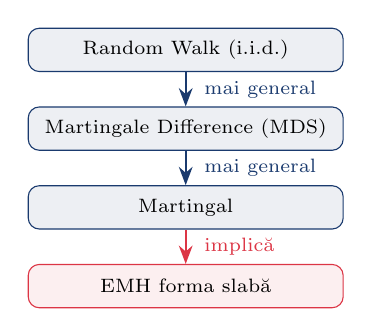
\begin{tikzpicture}[
    every node/.style={font=\scriptsize}
]
\node[draw=MainBlue, fill=MainBlue!8, rounded corners, minimum width=4cm, minimum height=0.55cm] (rw) at (0,3) {Random Walk (i.i.d.)};
\node[draw=MainBlue, fill=MainBlue!8, rounded corners, minimum width=4cm, minimum height=0.55cm] (mds) at (0,2) {Martingale Difference (MDS)};
\node[draw=MainBlue, fill=MainBlue!8, rounded corners, minimum width=4cm, minimum height=0.55cm] (mart) at (0,1) {Martingal};
\node[draw=Crimson, fill=Crimson!8, rounded corners, minimum width=4cm, minimum height=0.55cm] (emh) at (0,0) {EMH forma slabă};
\draw[-{Stealth}, MainBlue, thick] (rw) -- (mds) node[midway, right=3pt] {mai general};
\draw[-{Stealth}, MainBlue, thick] (mds) -- (mart) node[midway, right=3pt] {mai general};
\draw[-{Stealth}, Crimson, thick] (mart) -- (emh) node[midway, right=3pt] {implică};
\end{tikzpicture}
\end{center}
\end{column}
\end{columns}
\end{cminipage}
\end{frame}

\begin{frame}[shrink=25]{Random walk vs non-random walk --- vizual și statistic}
\begin{cminipage}{0.95\textwidth}
\begin{columns}[T]
\begin{column}{0.66\textwidth}
\centering
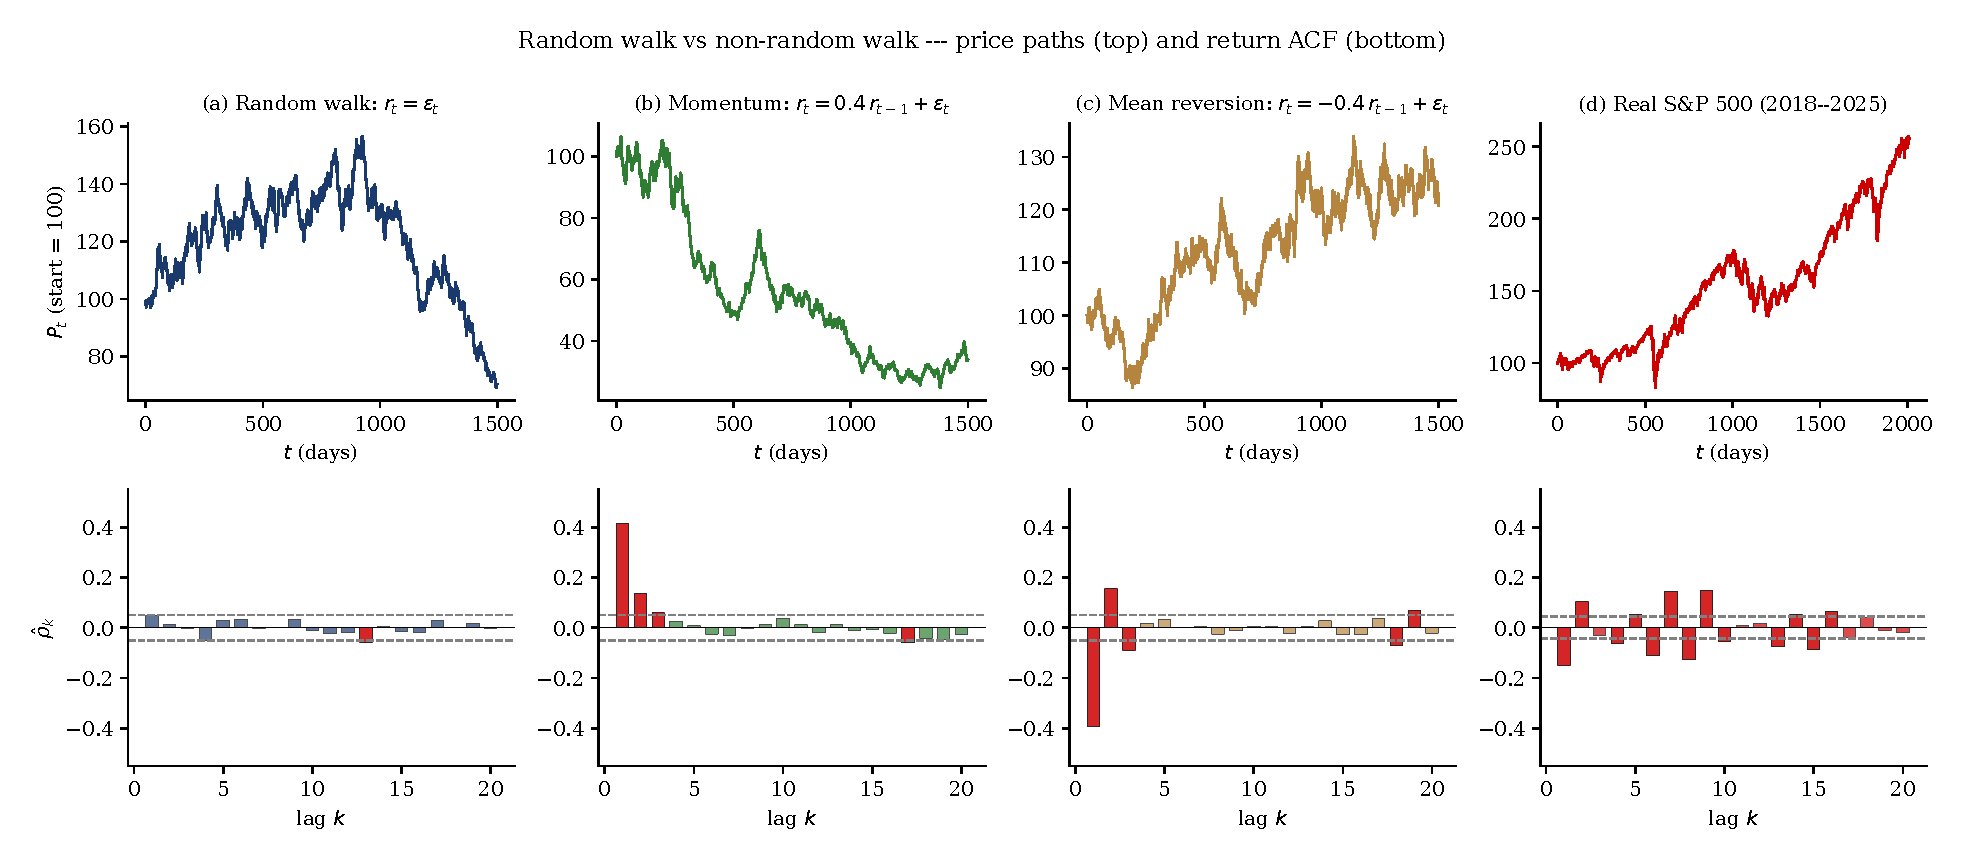
\includegraphics[width=\linewidth]{sfm_ch4_rw_vs_nonrw.pdf}
\end{column}
\begin{column}{0.32\textwidth}
\footnotesize
\begin{itemize}\setlength{\itemsep}{0pt}
    \item \textbf{Citire grafic}
    \begin{itemize}\setlength{\itemsep}{0pt}
        \item Sus: 4 traiectorii ,,trending''
        \item Jos: ACF distinge RW de non-RW
    \end{itemize}
    \item \textbf{$\hat\rho_1$ observat}
    \begin{itemize}\setlength{\itemsep}{0pt}
        \item RW: $0{,}05$ (în bandă)
        \item Momentum: $0{,}42$
        \item Mean rev.: $-0{,}39$
        \item S\&P 500: $-0{,}15$
    \end{itemize}
    \item Date: $T=1500$ simulate; S\&P 500: $n=2009$
    \item Lecție: doar testele decid
\end{itemize}
\end{column}
\end{columns}
\vspace{0.1cm}
\begin{exampleblock}{Modelele care generează cele patru traiectorii}
\footnotesize
\begin{columns}[T]
\begin{column}{0.32\textwidth}
\textbf{Randament și preț}
\[
    r_t = \ln\!\frac{P_t}{P_{t-1}}, \quad P_t = P_{t-1}\,e^{r_t}
\]
\end{column}
\begin{column}{0.32\textwidth}
\textbf{Random walk (RW)}
\[
    r_t = \mu + \varepsilon_t, \;\; \varepsilon_t \overset{\text{iid}}{\sim} \mathcal{N}(0,\sigma^2)
\]
\end{column}
\begin{column}{0.34\textwidth}
\textbf{Non-RW (AR(1))}
\[
    r_t = \mu + \phi\, r_{t-1} + \varepsilon_t
\]
$\phi > 0$: momentum; $\phi < 0$: mean reversion
\end{column}
\end{columns}
\end{exampleblock}
\end{cminipage}
\vspace{0.05cm}
\quantlet{SFM\_ch4\_rw\_vs\_nonrw}{https://colab.research.google.com/github/QuantLet/Stat_fin_markets/blob/master/Ch_04/SFM_ch4_rw_vs_nonrw/SFM_ch4_rw_vs_nonrw.ipynb}
\end{frame}

\begin{frame}[shrink=15]{S\&P 500 real vs random walk simulat}
\begin{cminipage}{0.95\textwidth}
\begin{columns}[T]
\begin{column}{0.66\textwidth}
\centering
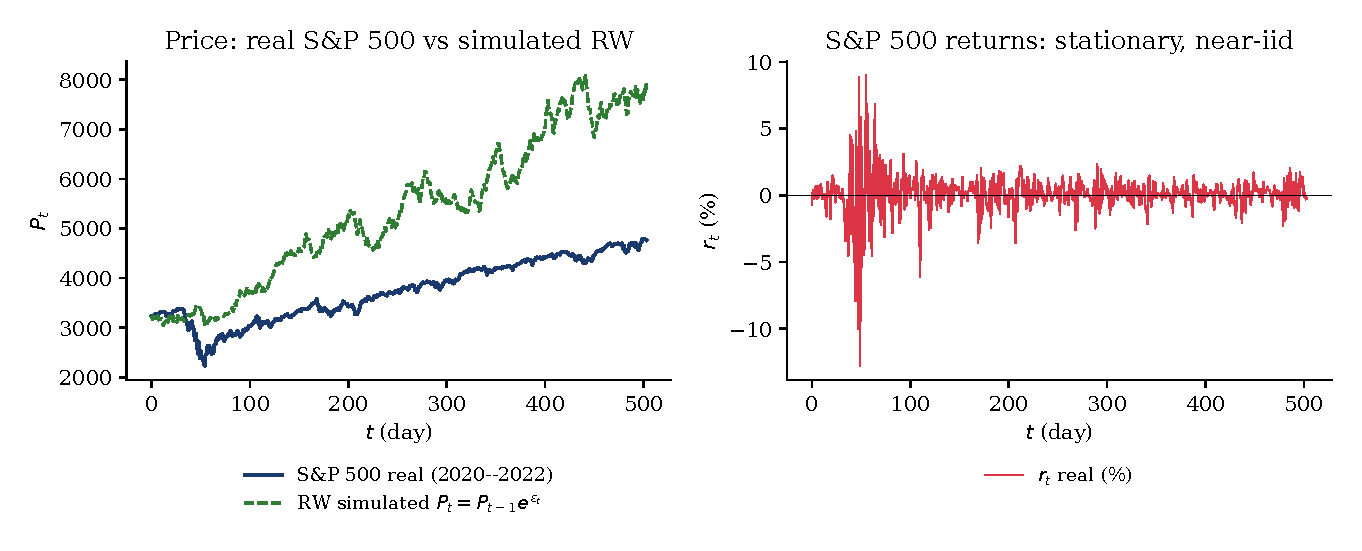
\includegraphics[width=\linewidth]{sfm_ch4_rw_sim.pdf}
\end{column}
\begin{column}{0.32\textwidth}
\footnotesize
\begin{itemize}\setlength{\itemsep}{0pt}
    \item \textbf{Panoul stânga}
    \begin{itemize}\setlength{\itemsep}{0pt}
        \item S\&P 500 real (2020--2022)
        \item RW simulat $P_t = P_{t-1} e^{\varepsilon_t}$
        \item Vizual indistinguibile
    \end{itemize}
    \item \textbf{Panoul dreapta}
    \begin{itemize}\setlength{\itemsep}{0pt}
        \item Randamente zilnice S\&P
        \item Staționare, oscilează în jur de $0$
        \item $\bar r \approx 0{,}075\%$/zi
        \item $\hat\sigma \approx 1{,}65\%$/zi
    \end{itemize}
    \item \textbf{Punctul cheie}
    \begin{itemize}\setlength{\itemsep}{0pt}
        \item Prețurile par non-staționare
        \item Randamentele sunt staționare
    \end{itemize}
\end{itemize}
\end{column}
\end{columns}
\end{cminipage}
\vspace{0.05cm}
\quantlet{SFM\_ch4\_rw\_sim}{https://colab.research.google.com/github/QuantLet/Stat_fin_markets/blob/master/Ch_04/SFM_ch4_rw_sim/SFM_ch4_rw_sim.ipynb}
\end{frame}

\begin{frame}[shrink=15]{Exercițiul 1: Proprietatea de martingal}
\begin{cminipage}{0.95\textwidth}
\begin{block}{Problemă}
\begin{itemize}\setlength{\itemsep}{0pt}
    \item Fie $P_t = P_{t-1} + \varepsilon_t$ cu $\varepsilon_t \sim \mathcal{N}(0, \sigma^2)$ i.i.d. Arătați că $\E[P_{t+1} | \Omega_t] = P_t$ (proprietatea de martingal).
\end{itemize}
\end{block}

\begin{exampleblock}{Rezolvare}
\begin{itemize}\setlength{\itemsep}{0pt}
    \item Din modelul random walk: $P_{t+1} = P_t + \varepsilon_{t+1}$
    \item Aplicăm speranța condițională:
$$\E[P_{t+1} | \Omega_t] = \E[P_t + \varepsilon_{t+1} | \Omega_t] = P_t + \E[\varepsilon_{t+1} | \Omega_t]$$
    \item Deoarece $\varepsilon_{t+1}$ este independent de $\Omega_t$ și $\E[\varepsilon_{t+1}] = 0$:
$$\E[P_{t+1} | \Omega_t] = P_t + 0 = P_t \quad \checkmark$$
    \item \textbf{Concluzie:} Prețul curent este cea mai bună predicție pentru prețul viitor.
    \item \textbf{Extensie:} $\E[P_{t+k} | \Omega_t] = P_t$ pentru orice $k \geq 1$ (prin inducție).
\end{itemize}
\end{exampleblock}
\end{cminipage}
\end{frame}

\begin{frame}[shrink=15]{Exercițiul 1 cont.: Implicații practice}
\begin{cminipage}{0.95\textwidth}
\begin{columns}[T]
\begin{column}{0.48\textwidth}
\begin{block}{Ce implică martingalul?}
\begin{itemize}\setlength{\itemsep}{0pt}
    \item Randamentele sunt \textbf{impredictibile}: $\E[r_{t+1} | \Omega_t] = 0$
    \item Nicio strategie bazată pe prețuri trecute nu poate genera profit sistematic
    \item Analiza tehnică (medii mobile, RSI, MACD) nu are putere predictivă
    \item ,,Piața nu are memorie''
\end{itemize}
\end{block}
\end{column}
\begin{column}{0.48\textwidth}
\begin{block}{Ce NU implică}
\begin{itemize}\setlength{\itemsep}{0pt}
    \item Prețurile nu sunt ,,aleatoare'' --- reflectă fundamentalele
    \item Volatilitatea poate fi predictibilă (GARCH): $\Var(r_{t+1}|\Omega_t) \neq \text{const}$
    \item Primă de risc: $\E[r_{t+1}|\Omega_t] = \mu > 0$ (sub-martingal)
    \item Piața poate fi eficientă \textbf{și} volatilă
\end{itemize}
\end{block}
\end{column}
\end{columns}

\vspace{0.2cm}
\begin{alertblock}{Atenție}
\begin{itemize}\setlength{\itemsep}{0pt}
    \item \textbf{EMH nu presupune normalitate} ($r_t \not\sim \mathcal{N}(0, \sigma^2)$)
    \begin{itemize}\setlength{\itemsep}{0pt}
        \item Randamentele pot avea cozi grele
        \item Volatilitate variabilă (GARCH) este compatibilă
    \end{itemize}
    \item \textbf{Condiția cheie:} impredictibilitatea, nu normalitatea
\end{itemize}
\end{alertblock}
\end{cminipage}
\end{frame}

%=============================================================================
% PARTEA II: AUTOCORELAȚIE ȘI LJUNG--BOX
%=============================================================================
\section{Partea II: Autocorelație și Ljung--Box}

\begin{frame}[shrink=15]{Testul de autocorelație --- ACF (Autocorrelation Function)}
\begin{cminipage}{0.95\textwidth}
\begin{columns}[T]
\begin{column}{0.48\textwidth}
\begin{block}{Autocorelația eșantion}
\begin{itemize}\setlength{\itemsep}{0pt}
    \item $\hat\rho_k = \frac{\sum_{t=k+1}^{T}(r_t - \bar r)(r_{t-k} - \bar r)}{\sum_{t=1}^{T}(r_t - \bar r)^2}$
    \item Sub RW: $\hat\rho_k \approx \mathcal{N}(0, 1/T)$
    \item Banda de încredere 95\%: $\pm 1{,}96/\sqrt{T}$
\end{itemize}
\end{block}
\end{column}
\begin{column}{0.48\textwidth}
\begin{block}{Ljung--Box $Q(m)$}
\begin{itemize}\setlength{\itemsep}{0pt}
    \item $Q(m) = T(T+2)\sum_{k=1}^{m}\frac{\hat\rho_k^2}{T-k}$
    \item Sub $H_0$: $Q \sim \chi^2_m$
    \item $H_0$: toate $\rho_1 \ldots \rho_m$ sunt zero
\end{itemize}
\end{block}
\end{column}
\end{columns}

\vspace{0.15cm}
\begin{alertblock}{Rezultat empiric clasic (Lo \& MacKinlay, 1988)}
\begin{itemize}\setlength{\itemsep}{0pt}
    \item Pe indici majori: $|\hat\rho_k| < 0{,}05$ la toate lag-urile $k$
    \item Statistic semnificativ (pe $T$ mare), economic nesemnificativ
    \item Compatibil cu EMH slabă după costuri de tranzacționare
\end{itemize}
\end{alertblock}
\end{cminipage}
\end{frame}

\begin{frame}[shrink=15]{Exercițiul 2: Autocorelație lag 1 și lag 2}
\begin{cminipage}{0.95\textwidth}
\begin{block}{Problemă}
\begin{itemize}\setlength{\itemsep}{0pt}
    \item Date: randamente zilnice $r_1, \ldots, r_{10}$: 0.02, $-$0.01, 0.03, $-$0.02, 0.01, 0.04, $-$0.03, 0.02, $-$0.01, 0.03.
    \item Calculați $\hat\rho_1$, $\hat\rho_2$ și statistica Ljung--Box $Q(2)$.
\end{itemize}
\end{block}

\begin{exampleblock}{Rezolvare --- Autocorelație}
\small
\begin{itemize}\setlength{\itemsep}{0pt}
    \item Media: $\bar{r} = \frac{1}{10}\sum r_i = 0{,}008$
    \item Autocovarianță: $\hat\gamma_k = \frac{1}{n}\sum_{t=k+1}^{n}(r_t - \bar{r})(r_{t-k} - \bar{r})$
    \item $\hat\gamma_0 = 0{,}000436$, \; $\hat\gamma_1 = -0{,}000298$, \; $\hat\gamma_2 = 0{,}000062$
    \item Autocorelație: $\hat\rho_k = \hat\gamma_k / \hat\gamma_0$
    \item $\hat\rho_1 = -0{,}000298 / 0{,}000436 \approx \mathbf{-0{,}683}$
    \item $\hat\rho_2 = 0{,}000062 / 0{,}000436 \approx \mathbf{0{,}142}$
    \item \textbf{Interpretare:} Autocorelație negativă la lag 1 --- posibil efect de mean reversion
\end{itemize}
\end{exampleblock}
\end{cminipage}
\end{frame}

\begin{frame}[shrink=15]{Exercițiul 2 cont.: Statistica Ljung--Box}
\begin{cminipage}{0.95\textwidth}
\begin{exampleblock}{Rezolvare --- Ljung--Box}
\small
\begin{itemize}\setlength{\itemsep}{0pt}
    \item \textbf{Formula:} $Q(m) = n(n+2)\sum_{k=1}^{m}\frac{\hat\rho_k^2}{n-k}$
    \item Cu $n = 10$, $m = 2$:
$Q(2) = 120 \left[\frac{0{,}467}{9} + \frac{0{,}020}{8}\right]
= 120 [0{,}0519 + 0{,}0025] = \mathbf{6{,}53}$
    \item Sub $H_0$: $Q(2) \sim \chi^2(2)$. Valoare critică la 5\%: $\chi^2_{0{,}05}(2) = 5{,}99$.
    \item $Q(2) = 6{,}53 > 5{,}99$ $\Rightarrow$ \textcolor{Crimson}{\textbf{Respingem $H_0$}} la nivel de 5\%.
    \item \textbf{Concluzie:} Randamentele prezintă autocorelație semnificativă --- evidență contra EMH slabe.
\end{itemize}
\end{exampleblock}

\begin{alertblock}{Notă}
\begin{itemize}\setlength{\itemsep}{0pt}
    \item \textbf{Eșantion mic} ($n = 10$): rezultatul nu este reprezentativ
    \item Pe eșantioane mari ($n > 250$): autocorelațiile pe indici mari sunt de obicei nesemnificative
\end{itemize}
\end{alertblock}
\end{cminipage}
\end{frame}

\begin{frame}[shrink=15]{ACF S\&P 500 2000--2024}
\begin{cminipage}{0.95\textwidth}
\begin{columns}[T]
\begin{column}{0.6\textwidth}
\centering
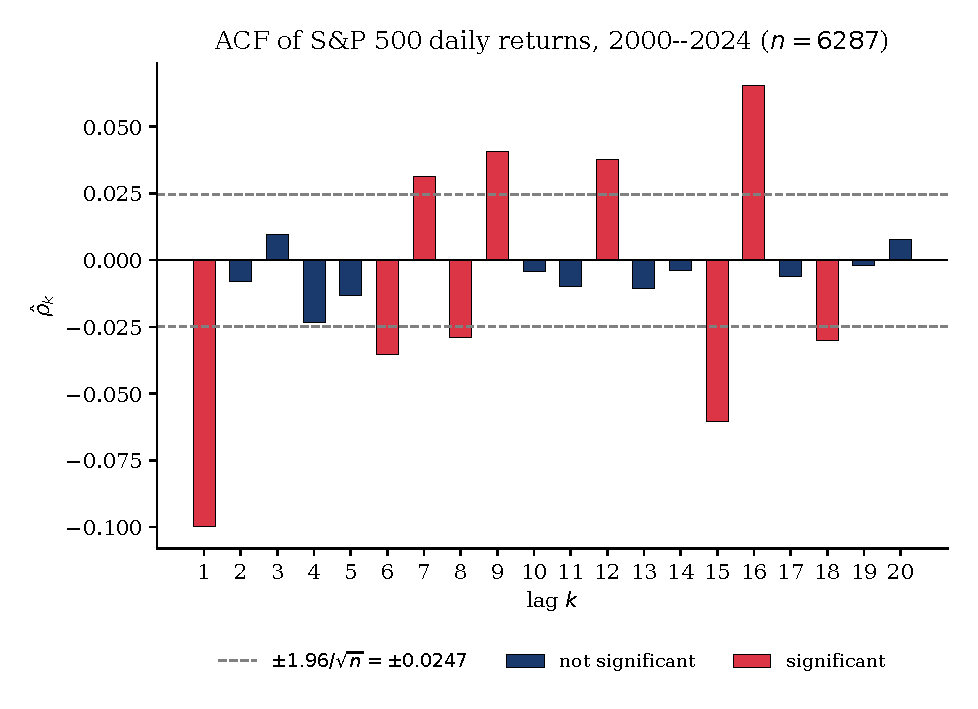
\includegraphics[width=\linewidth]{sfm_ch4_acf_sp500.pdf}
\end{column}
\begin{column}{0.37\textwidth}
\begin{itemize}\setlength{\itemsep}{0pt}
    \item Date: \texttt{\^{}GSPC} zilnic
    \begin{itemize}\setlength{\itemsep}{0pt}
        \item $n = 6.287$ observații zilnice
        \item Banda: $\pm 1{,}96/\sqrt{n} \approx \pm 0{,}025$
    \end{itemize}
    \item Observații
    \begin{itemize}\setlength{\itemsep}{0pt}
        \item 9 lag-uri depășesc banda (roșu): $\{1, 6, 7, 8, 9, 12, 15, 16, 18\}$
        \item max $|\hat\rho_k| = 0{,}10$ (lag 1, $\hat\rho_1=-0{,}10$)
        \item Ljung--Box $Q(10)=97{,}6$ vs critic $18{,}3$, $p<10^{-16}$
    \end{itemize}
    \item Verdict
    \begin{itemize}\setlength{\itemsep}{0pt}
        \item \alert{Statistic}: RW \textbf{respinsă} clar
        \item \textbf{Economic}: $R^2 = \hat\rho_1^2 = 0{,}99\%$ --- după $\sim$5bp costuri tranzacționare, neexploatabil
        \item ,,Efficiently inefficient'' (Pedersen, 2015)
    \end{itemize}
\end{itemize}
\end{column}
\end{columns}
\end{cminipage}
\vspace{0.05cm}
\quantlet{SFM\_ch4\_acf\_sp500}{https://colab.research.google.com/github/QuantLet/Stat_fin_markets/blob/master/Ch_04/SFM_ch4_acf_sp500/SFM_ch4_acf_sp500.ipynb}
\end{frame}

\begin{frame}[shrink=15]{ACF randamente vs ACF randamente la pătrat (S\&P 500)}
\begin{cminipage}{0.95\textwidth}
\begin{columns}[T]
\begin{column}{0.66\textwidth}
\centering
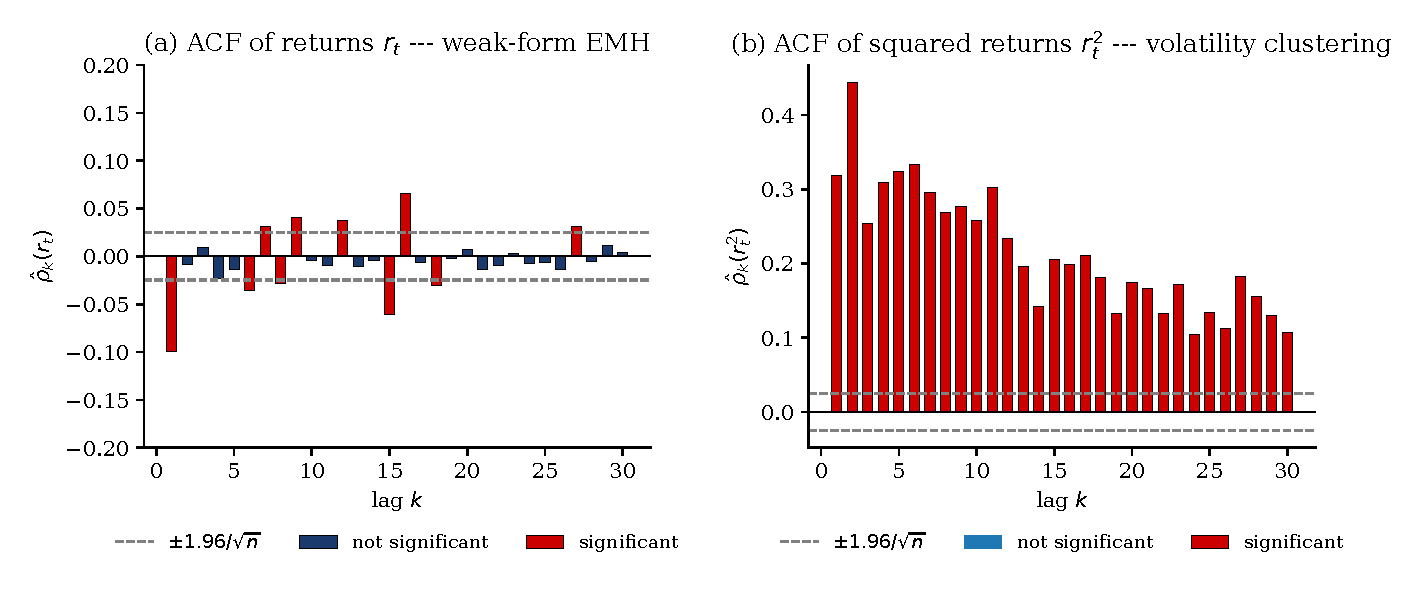
\includegraphics[width=\linewidth]{sfm_ch4_acf_returns_vs_squared.pdf}
\end{column}
\begin{column}{0.32\textwidth}
\footnotesize
\begin{itemize}\setlength{\itemsep}{0pt}
    \item \textbf{Citire grafic}
    \begin{itemize}\setlength{\itemsep}{0pt}
        \item (a): ACF$(r_t)$ \emph{aproape} de bandă; câteva lag-uri ies, dar magnitudine mică
        \item (b): ACF$(r_t^2)$ \emph{toate} bare semnificative, descreștere lentă (GARCH)
    \end{itemize}
    \item \textbf{Empiric} ($n = 6287$, banda $\pm 0{,}025$)
    \begin{itemize}\setlength{\itemsep}{0pt}
        \item max $|\hat\rho(r_t)| = 0{,}10$ (lag 1)
        \item max $\hat\rho(r_t^2) = 0{,}44$ (lag 1)
        \item Raport $\approx 4{,}4\times$ mai puternic pe $r_t^2$
    \end{itemize}
    \item \textbf{Lecție cheie}
    \begin{itemize}\setlength{\itemsep}{0pt}
        \item EMH cere doar randamente impredictibile
        \item Volatilitatea poate fi predictibilă (EMH + GARCH)
    \end{itemize}
\end{itemize}
\end{column}
\end{columns}
\end{cminipage}
\vspace{0.05cm}
\quantlet{SFM\_ch4\_acf\_returns\_vs\_squared}{https://colab.research.google.com/github/QuantLet/Stat_fin_markets/blob/master/Ch_04/SFM_ch4_acf_returns_vs_squared/SFM_ch4_acf_returns_vs_squared.ipynb}
\end{frame}

\begin{frame}[shrink=15]{Exercițiul Ljung--Box pe BVB --- enunț}
\begin{cminipage}{0.95\textwidth}
\begin{block}{Enunț}
\begin{itemize}\setlength{\itemsep}{0pt}
    \item Pe $T = 250$ randamente zilnice BET se observă:
    \begin{itemize}\setlength{\itemsep}{0pt}
        \item $\hat\rho_1 = 0{,}12$; $\hat\rho_2 = 0{,}05$; $\hat\rho_3 = 0{,}03$
        \item $\hat\rho_4 = -0{,}02$; $\hat\rho_5 = 0{,}08$
    \end{itemize}
\end{itemize}
\end{block}

\begin{itemize}\setlength{\itemsep}{0pt}
    \item \textbf{Cerințe}
    \begin{itemize}\setlength{\itemsep}{0pt}
        \item Calculați $Q(5)$ folosind $Q(m) = T(T+2)\sum_{k=1}^{m}\frac{\hat\rho_k^2}{T-k}$
        \item Testați $H_0$ la $\alpha = 5\%$ cu $\chi^2_5(0{,}05) = 11{,}07$
        \item Interpretați economic vs EMH slabă
    \end{itemize}
\end{itemize}
\end{cminipage}
\end{frame}

\begin{frame}[shrink=15]{Exercițiul Ljung--Box pe BVB --- rezolvare}
\begin{cminipage}{0.95\textwidth}
\begin{exampleblock}{Rezolvare}
\begin{itemize}\setlength{\itemsep}{0pt}
    \item \textbf{Calculul $Q(5)$}
    \begin{itemize}\setlength{\itemsep}{0pt}
        \item $T(T+2) = 250 \cdot 252 = 63.000$
        \item Sumă: $\frac{0{,}12^2}{249} + \frac{0{,}05^2}{248} + \frac{0{,}03^2}{247} + \frac{0{,}02^2}{246} + \frac{0{,}08^2}{245}$
        \item $= 5{,}78 \cdot 10^{-5} + 1{,}01 \cdot 10^{-5} + 3{,}64 \cdot 10^{-6} + 1{,}63 \cdot 10^{-6} + 2{,}61 \cdot 10^{-5}$
        \item Total $\approx 9{,}71 \cdot 10^{-5}$
        \item $Q(5) = 63.000 \cdot 9{,}71 \cdot 10^{-5} \approx \mathbf{6{,}12}$
    \end{itemize}
    \item \textbf{Decizia}
    \begin{itemize}\setlength{\itemsep}{0pt}
        \item $Q(5) = 6{,}12 < 11{,}07 \Rightarrow$ nu respingem $H_0$ la 5\%
    \end{itemize}
    \item \textbf{Interpretare}
    \begin{itemize}\setlength{\itemsep}{0pt}
        \item La nivel 5\%, BET este compatibil cu EMH slabă
        \item Notă: $\hat\rho_1 = 0{,}12$ ar putea fi relevant pe eșantion mai mare
    \end{itemize}
\end{itemize}
\end{exampleblock}
\end{cminipage}
\end{frame}

%=============================================================================
% PARTEA III: RUNS TEST
%=============================================================================
\section{Partea III: Runs test}

\begin{frame}[shrink=15]{Exercițiul 3: Runs test --- secvențe de semne}
\begin{cminipage}{0.95\textwidth}
\begin{block}{Problemă}
\begin{itemize}\setlength{\itemsep}{0pt}
    \item Secvența de semne a randamentelor: $+, -, +, -, +, +, -, +, -, +$.
    \item Calculați $R$ (numărul de runs), $\E[R]$, $\Var(R)$ și statistica $Z$.
\end{itemize}
\end{block}

\begin{exampleblock}{Rezolvare}
\small
\begin{itemize}\setlength{\itemsep}{0pt}
    \item Grupuri: $(+)(-)(+)(-)(+,+)(-)(+)(-)(+)$ $\Rightarrow$ $R = 9$ runs
    \item $n_+ = 6$ (pozitive), $n_- = 4$ (negative), $n = 10$
    \item Speranța: $\E[R] = \frac{2 n_+ n_-}{n} + 1 = \frac{2 \cdot 6 \cdot 4}{10} + 1 = 5{,}8$
    \item Varianța: $\Var(R) = \frac{2n_+n_-(2n_+n_- - n)}{n^2(n-1)} = \frac{2 \cdot 6 \cdot 4 \cdot (48-10)}{100 \cdot 9} = \frac{1824}{900} = 2{,}027$
    \item Statistica $Z$: $\displaystyle Z = \frac{R - \E[R]}{\sqrt{\Var(R)}} = \frac{9 - 5{,}8}{\sqrt{2{,}027}} = \frac{3{,}2}{1{,}424} = \mathbf{2{,}247}$
    \item $|Z| = 2{,}247 > 1{,}96$ $\Rightarrow$ \textcolor{Crimson}{\textbf{Respingem $H_0$}} la 5\%: prea multe runs (alternare excesivă)
    \item \textbf{Interpretare:} Alternare frecventă sugerează mean reversion pe termen scurt
\end{itemize}
\end{exampleblock}
\end{cminipage}
\end{frame}

%=============================================================================
% PARTEA IV: VARIANCE RATIO
%=============================================================================
\section{Partea IV: Variance Ratio}

\begin{frame}[shrink=10]{VR test 1/3 --- intuiție și ipoteze}
\begin{cminipage}{0.95\textwidth}
\begin{block}{Intuiție}
\footnotesize
Sub random walk i.i.d., suma a $q$ randamente are varianță $= q \cdot \Var(r_t)$ (varianța crește \emph{liniar} cu orizontul). Orice deviere de la liniaritate semnalează \emph{autocorelație}.
\end{block}
\begin{block}{Definiție și identitate}
\footnotesize
\[
    VR(q) = \frac{\Var(r_t + r_{t+1} + \cdots + r_{t+q-1})}{q \cdot \Var(r_t)} = 1 + 2\sum_{k=1}^{q-1}\!\left(1 - \tfrac{k}{q}\right)\rho_k
\]
\begin{itemize}\setlength{\itemsep}{0pt}
    \item Toate $\rho_k = 0$ ($k \geq 1$) $\Leftrightarrow$ $VR(q) = 1$ pentru orice $q$
    \item $\rho_k$ apar ponderate: lag-uri scurte au pondere mai mare
\end{itemize}
\end{block}
\begin{exampleblock}{Ipotezele testului}
\footnotesize
\begin{itemize}\setlength{\itemsep}{0pt}
    \item $H_0$: $VR(q) = 1$ --- compatibil cu random walk slabă
    \item $H_1$ \emph{bilateral}: $VR(q) \neq 1$ --- testul standard
    \item $H_1$ \emph{unilateral momentum}: $VR(q) > 1$ ($\rho_k > 0$ net pe lag-uri $\leq q-1$)
    \item $H_1$ \emph{unilateral mean rev.}: $VR(q) < 1$ ($\rho_k < 0$ net)
\end{itemize}
\end{exampleblock}
\end{cminipage}
\end{frame}

\begin{frame}[shrink=10]{VR test 2/3 --- algoritm pas-cu-pas și erori standard}
\begin{cminipage}{0.95\textwidth}
\begin{columns}[T]
\begin{column}{0.46\textwidth}
\begin{exampleblock}{Algoritm Lo--MacKinlay (1988)}
\footnotesize
\begin{enumerate}\setlength{\itemsep}{0pt}
    \item Log-randamente: $r_t = \log(P_t/P_{t-1})$, $T$ obs.
    \item Media: $\hat\mu = \frac{1}{T}\sum r_t$
    \item $\hat\sigma^2_a = \frac{1}{T-1}\sum (r_t - \hat\mu)^2$
    \item Cumulate: $R_t(q) = \sum_{i=0}^{q-1} r_{t+i}$
    \item $\hat\sigma^2_c(q) = \frac{1}{T-q}\sum (R_t(q) - q\hat\mu)^2$
    \item $\widehat{VR}(q) = \hat\sigma^2_c(q) / (q \cdot \hat\sigma^2_a)$
    \item $Z = (\widehat{VR}(q) - 1) / SE$ \quad (vezi dreapta)
\end{enumerate}
\end{exampleblock}
\end{column}
\begin{column}{0.52\textwidth}
\begin{block}{Erori standard --- alegerea contează}
\footnotesize
\textbf{Homoscedastic} ($r_t$ i.i.d. normal):
\[
    SE = \sqrt{\frac{2(2q-1)(q-1)}{3qT}} \;\approx\; \sqrt{\frac{2(q-1)}{T}}
\]
\textbf{Heterosc-robust} (clustering volatilitate):
\[
    SE^* = \sqrt{\phi^*(q)/T}, \quad \phi^*(q) = \sum_{k=1}^{q-1} \left[\tfrac{2(q-k)}{q}\right]^2 \hat\delta_k
\]
\[
    \hat\delta_k = \frac{T \sum_{t=k+1}^T (r_t - \hat\mu)^2 (r_{t-k} - \hat\mu)^2}{\left[\sum_t (r_t - \hat\mu)^2\right]^2}
\]
\begin{itemize}\setlength{\itemsep}{0pt}
    \item $\hat\delta_k$ = autocovarianța \emph{pătratelor} reziduurilor
    \item Sub heteroscedasticitate, $SE^*$ este mai mare ca $SE$ $\Rightarrow$ test mai conservator
    \item \alert{Recomandare}: folosește mereu $SE^*$
\end{itemize}
\end{block}
\end{column}
\end{columns}
\end{cminipage}
\end{frame}

\begin{frame}[shrink=10]{VR test 3/3 --- decizie, interpretare și capcane}
\begin{cminipage}{0.95\textwidth}
\begin{columns}[T]
\begin{column}{0.5\textwidth}
\begin{block}{Regula de decizie}
\footnotesize
\begin{itemize}\setlength{\itemsep}{0pt}
    \item $|Z^*| > 1{,}96 \Rightarrow$ respingem $H_0$ la $\alpha = 5\%$
    \item $|Z^*| > 2{,}576 \Rightarrow$ respingem la $\alpha = 1\%$
    \item Echivalent: $1 \notin [\widehat{VR}(q) \pm 1{,}96 \cdot SE^*]$
\end{itemize}
\end{block}
\begin{exampleblock}{Interpretare}
\footnotesize
\begin{itemize}\setlength{\itemsep}{0pt}
    \item $\widehat{VR}(q) \approx 1$: compatibil cu RW
    \item $\widehat{VR}(q) > 1$: \emph{momentum}, $\rho_k > 0$ net
    \item $\widehat{VR}(q) < 1$: \emph{mean reversion}, $\rho_k < 0$ net
    \item Magnitudine: $\widehat{VR}(2) - 1 \approx 2\hat\rho_1$
\end{itemize}
\end{exampleblock}
\end{column}
\begin{column}{0.5\textwidth}
\begin{exampleblock}{Tipare empirice tipice}
\footnotesize
\begin{itemize}\setlength{\itemsep}{0pt}
    \item Acțiuni dezvoltate (S\&P): $VR \in [0{,}8;\, 1{,}0]$
    \item Crypto (BTC, ETH): $VR > 1$ pe lung --- momentum
    \item FX major (EUR/USD): $VR \approx 1$ --- aproape RW
    \item Emerging (BVB, EEM): $VR < 0{,}9$ --- thin trading
\end{itemize}
\end{exampleblock}
\begin{alertblock}{Capcane}
\footnotesize
\begin{itemize}\setlength{\itemsep}{0pt}
    \item Folosește $SE^*$; $SE$ homoscedastic supra-respinge
    \item Cozi grele ($\alpha < 2$): asimptotica eșuează $\Rightarrow$ bootstrap
    \item $q$ prea mare ($> T/4$): putere $\to 0$
    \item Ex-post selection $q^* \Rightarrow$ data snooping; folosește MVR
    \item Statistic $\neq$ economic: $R^2 = \hat\rho_1^2$ adesea $< 1\%$
\end{itemize}
\end{alertblock}
\end{column}
\end{columns}
\end{cminipage}
\end{frame}

\begin{frame}[shrink=15]{Exercițiul 4: VR(2) și VR(5) --- calcul manual}
\begin{cminipage}{0.95\textwidth}
\begin{block}{Problemă}
\begin{itemize}\setlength{\itemsep}{0pt}
    \item Date: randamente zilnice $r_1, \ldots, r_{10}$: 0.02, $-$0.01, 0.03, $-$0.02, 0.01, 0.04, $-$0.03, 0.02, $-$0.01, 0.03.
    \item Calculați $VR(2)$ și $VR(5)$, interpretați.
\end{itemize}
\end{block}

\begin{exampleblock}{Rezolvare}
\small
\begin{itemize}\setlength{\itemsep}{0pt}
    \item \textbf{Definiție:} $VR(q) = \Var(r_t + \cdots + r_{t+q-1}) / (q \cdot \Var(r_t))$. Sub RW: $VR(q) = 1$
    \item $\hat\sigma^2_1 = \frac{1}{n-1}\sum(r_t - \bar{r})^2 = 0{,}000484$
    \item Randamente 2-perioade: 0{,}01, 0{,}02, 0{,}01, $-$0{,}01, 0{,}05, 0{,}01, $-$0{,}01, 0{,}01, 0{,}02
    \item $\hat\sigma^2_2 = 0{,}000325$ $\Rightarrow$ $VR(2) = 0{,}000325 / 0{,}000484 \approx \mathbf{0{,}672}$
    \item Randamente 5-perioade: 0{,}03, 0{,}05, 0{,}03, 0{,}00, 0{,}05, 0{,}05
    \item $\hat\sigma^2_5 = 0{,}000395$ $\Rightarrow$ $VR(5) = 0{,}000395 / 0{,}000484 \approx \mathbf{0{,}817}$
    \item $VR < 1$ $\Rightarrow$ \textbf{mean reversion}; $VR > 1$ $\Rightarrow$ \textbf{momentum}
\end{itemize}
\end{exampleblock}
\end{cminipage}
\end{frame}

\begin{frame}[shrink=15]{Profilul VR(q) pe 3 piețe (2015--2024)}
\begin{cminipage}{0.95\textwidth}
\begin{columns}[T]
\begin{column}{0.6\textwidth}
\centering
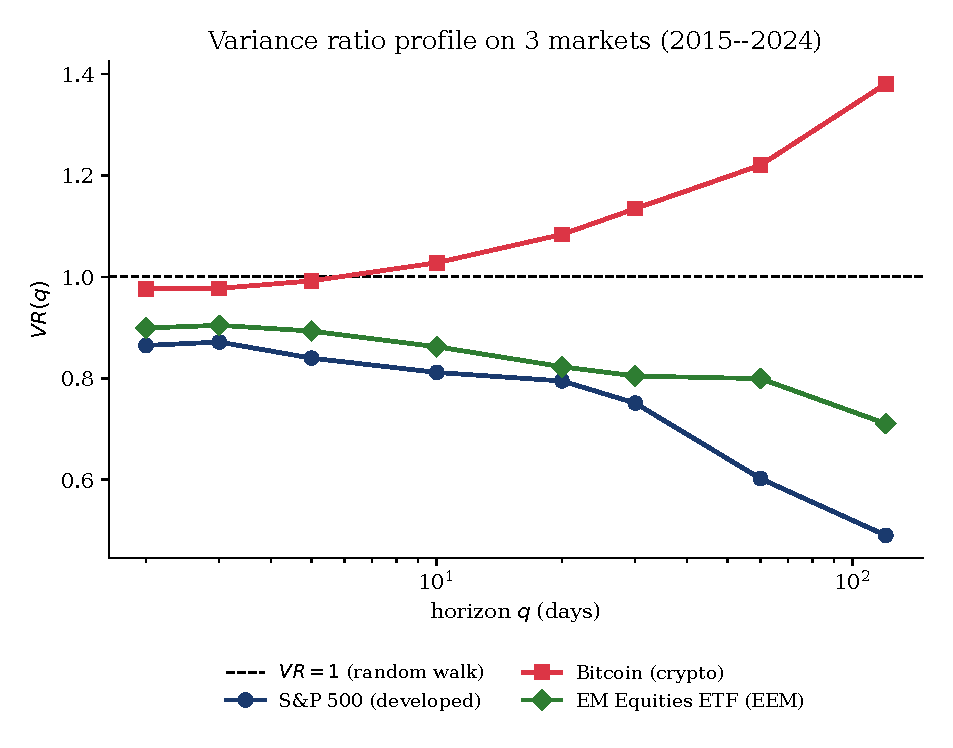
\includegraphics[width=\linewidth]{sfm_ch4_vr_profile.pdf}
\end{column}
\begin{column}{0.37\textwidth}
\begin{itemize}\setlength{\itemsep}{0pt}
    \item S\&P 500 (dezvoltată), $n = 2514$
    \begin{itemize}\setlength{\itemsep}{0pt}
        \item $\widehat{VR}(120) \approx 0{,}49$
        \item Mean reversion puternică pe orizont lung
    \end{itemize}
    \item Bitcoin (crypto), $n = 3651$
    \begin{itemize}\setlength{\itemsep}{0pt}
        \item $\widehat{VR}(120) \approx 1{,}38$
        \item Momentum puternic pe termen lung
    \end{itemize}
    \item EEM (emerging markets ETF, Exchange-Traded Fund), $n = 2514$
    \begin{itemize}\setlength{\itemsep}{0pt}
        \item $\widehat{VR}(120) \approx 0{,}71$
        \item Mean reversion moderată
    \end{itemize}
\end{itemize}
\end{column}
\end{columns}
\end{cminipage}
\vspace{0.05cm}
\quantlet{SFM\_ch4\_vr\_profile}{https://colab.research.google.com/github/QuantLet/Stat_fin_markets/blob/master/Ch_04/SFM_ch4_vr_profile/SFM_ch4_vr_profile.ipynb}
\end{frame}

\begin{frame}[shrink=15]{Variance ratio cu intervale de încredere 95\%}
\begin{cminipage}{0.95\textwidth}
\begin{columns}[T]
\begin{column}{0.6\textwidth}
\centering
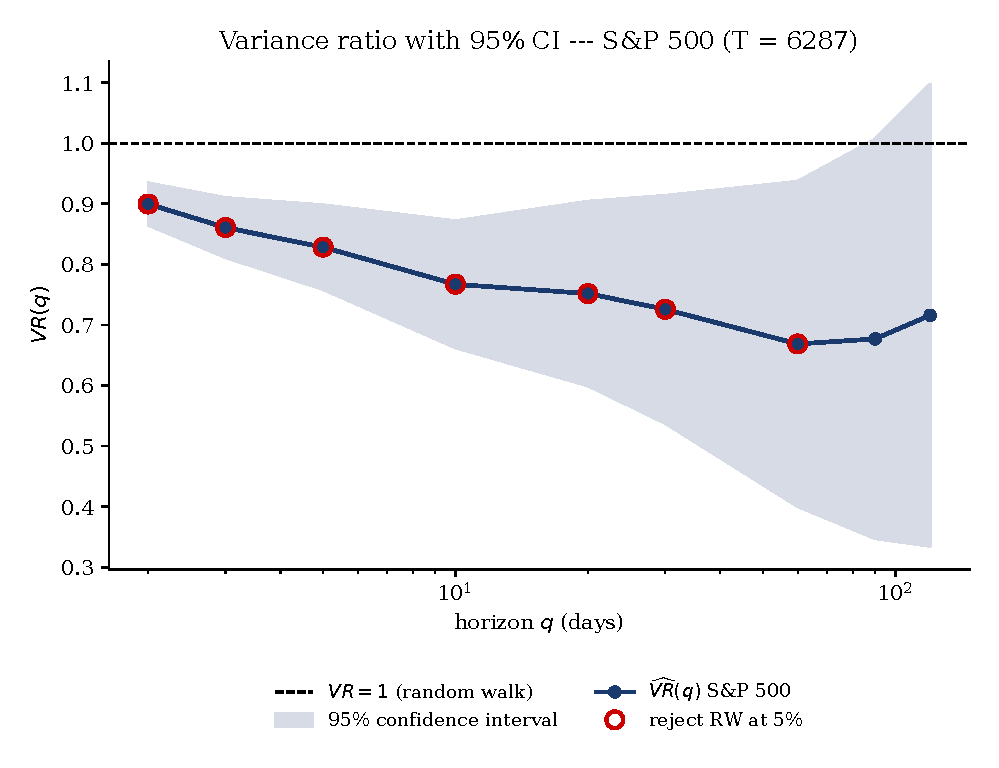
\includegraphics[width=\linewidth]{sfm_ch4_vr_with_ci.pdf}
\end{column}
\begin{column}{0.37\textwidth}
\begin{itemize}\setlength{\itemsep}{0pt}
    \item \textbf{Construcția IC} (interval de încredere)
    \begin{itemize}\setlength{\itemsep}{0pt}
        \item $\widehat{VR}(q) \pm 1{,}96 \cdot SE$
        \item $SE = \sqrt{2(q-1)/T}$
    \end{itemize}
    \item \textbf{Decizie}
    \begin{itemize}\setlength{\itemsep}{0pt}
        \item IC include $1$ $\Rightarrow$ nu respingem RW
        \item IC sub $1$ $\Rightarrow$ mean reversion
        \item IC peste $1$ $\Rightarrow$ momentum
    \end{itemize}
    \item \textbf{Observație S\&P 500} (2000--2024, $T = 6287$)
    \begin{itemize}\setlength{\itemsep}{0pt}
        \item $\widehat{VR}(120) \approx 0{,}72$ (eșantion lung)
        \item IC complet sub $1$ pe orizonturi mari
    \end{itemize}
    \item \textbf{Atenție:} valorile VR depind de eșantion
    \begin{itemize}\setlength{\itemsep}{0pt}
        \item 2015--2024 (slide ant.): $\widehat{VR}(120) \approx 0{,}49$
        \item 2000--2024 (aici): $\widehat{VR}(120) \approx 0{,}72$
        \item 2018--2025 (crypto chart): $\widehat{VR}(120) \approx 0{,}50$
    \end{itemize}
    \item \textbf{Avantaj IC vs $p$-value:} vede direct magnitudinea
\end{itemize}
\end{column}
\end{columns}
\end{cminipage}
\vspace{0.05cm}
\quantlet{SFM\_ch4\_vr\_with\_ci}{https://colab.research.google.com/github/QuantLet/Stat_fin_markets/blob/master/Ch_04/SFM_ch4_vr_with_ci/SFM_ch4_vr_with_ci.ipynb}
\end{frame}

\begin{frame}[shrink=35]{MVR 1/2 --- problema multiplicității și ipoteze}
\begin{cminipage}{0.95\textwidth}
\begin{block}{De ce un test multiplu?}
\footnotesize
\begin{itemize}\setlength{\itemsep}{0pt}
    \item În practică testăm VR la \emph{mai multe} orizonturi $q_1, \ldots, q_m$ (ex. $\{2,4,8,16\}$)
    \item Aplicarea individuală cu $\alpha = 5\%$ pe fiecare $\Rightarrow$ probabilitatea de \emph{cel puțin un} fals reject sub $H_0$:
    \[
        P(\text{fals reject} \mid H_0) \approx 1 - (1 - \alpha)^m \overset{m=4}{=} 1 - 0{,}95^4 \approx \mathbf{18{,}5\%}
    \]
    \item Concluzie: nivelul \emph{family-wise error rate} (FWER) este distorsionat dacă nu corectăm
\end{itemize}
\end{block}
\begin{columns}[T]
\begin{column}{0.5\textwidth}
\begin{exampleblock}{Ipoteza joint (Chow--Denning)}
\footnotesize
\begin{itemize}\setlength{\itemsep}{0pt}
    \item $H_0^{\text{joint}}: VR(q_i) = 1$ \emph{pentru toate} $i = 1, \ldots, m$
    \item $H_1^{\text{joint}}: \exists\, i$ astfel încât $VR(q_i) \neq 1$
    \item Testează \emph{simultan} dacă seria respectă RW pe toate orizonturile alese
\end{itemize}
\end{exampleblock}
\end{column}
\begin{column}{0.5\textwidth}
\begin{exampleblock}{Două abordări pentru FWER}
\footnotesize
\begin{itemize}\setlength{\itemsep}{0pt}
    \item \textbf{Bonferroni}: respinge dacă $\exists\, i: |Z^*(q_i)| > z_{1-\alpha/2m}$
    \begin{itemize}\setlength{\itemsep}{0pt}
        \item Pentru $m=4, \alpha=5\%$: prag $z_{0{,}99375} = 2{,}498$
        \item Conservator (ignoră dependența între $Z^*(q_i)$)
    \end{itemize}
    \item \textbf{Chow--Denning}: folosește direct distribuția maximului
    \begin{itemize}\setlength{\itemsep}{0pt}
        \item Ține cont de corelația naturală între statistici
        \item Putere mai mare ca Bonferroni
    \end{itemize}
\end{itemize}
\end{exampleblock}
\end{column}
\end{columns}
\begin{block}{Recomandări pentru $\{q_i\}$}
\footnotesize
\begin{itemize}\setlength{\itemsep}{0pt}
    \item Standardul Lo--MacKinlay: diadice $\{2, 4, 8, 16\}$ ($m=4$, scale: zi $\to$ lună)
    \item Evită $q$ apropiate (pierde putere) sau $q > T/4$ (SE explodează)
\end{itemize}
\end{block}
\end{cminipage}
\end{frame}

\begin{frame}[shrink=22]{MVR 2/2 --- procedură, decizie și interpretare}
\begin{cminipage}{0.95\textwidth}
\begin{columns}[T]
\begin{column}{0.5\textwidth}
\begin{exampleblock}{Algoritm Chow--Denning}
\footnotesize
\begin{enumerate}\setlength{\itemsep}{0pt}
    \item Alege $\{q_1, \ldots, q_m\}$ (recomandat: $\{2,4,8,16\}$)
    \item Pentru fiecare $q_i$, calc $\widehat{VR}(q_i)$ și $SE^*(q_i)$ heterosc-robust
    \item $Z^*(q_i) = (\widehat{VR}(q_i) - 1) / SE^*(q_i)$
    \item $\mathrm{MV1} = \max_{i} |Z^*(q_i)|$
    \item Identifică $q^* = \arg\max_i |Z^*(q_i)|$ (orizont critic)
    \item Compară cu valoare critică $\mathrm{SMM}_{\alpha}(m, \nu)$
\end{enumerate}
\end{exampleblock}
\begin{block}{Distribuția SMM (valori critice)}
\footnotesize
\begin{tabular}{rrrr}
\toprule
$m$ & $\alpha = 10\%$ & $\alpha = 5\%$ & $\alpha = 1\%$ \\
\midrule
$2$ & $1{,}960$ & $2{,}236$ & $2{,}807$ \\
$3$ & $2{,}120$ & $2{,}394$ & $2{,}935$ \\
$4$ & $2{,}228$ & $\mathbf{2{,}491}$ & $3{,}023$ \\
$6$ & $2{,}385$ & $2{,}609$ & $3{,}143$ \\
\bottomrule
\end{tabular}
\\[0.1cm]
\footnotesize Stoline \& Ury (1979), $\nu = \infty$
\end{block}
\end{column}
\begin{column}{0.5\textwidth}
\begin{exampleblock}{Regula de decizie și interpretare}
\footnotesize
\begin{itemize}\setlength{\itemsep}{0pt}
    \item $\mathrm{MV1} > \mathrm{SMM}_\alpha \Rightarrow$ respingem $H_0^{\text{joint}}$
    \item Concluzie: piața \emph{nu} e RW pe \emph{cel puțin un} $q_i$
    \item $q^*$ indică orizontul \emph{cel mai} predictibil
    \item $\mathrm{MV1} \leq \mathrm{SMM}_\alpha \Rightarrow$ \emph{nu} respingem (compatibil cu RW)
\end{itemize}
\end{exampleblock}
\begin{exampleblock}{Tipuri de respingere}
\footnotesize
\begin{itemize}\setlength{\itemsep}{0pt}
    \item Maximul la $q^* = 2$: dependență la \emph{1 zi} (mean rev. scurtă)
    \item Maximul la $q^* = 16$: persistență/momentum pe $\sim 3$ săptămâni
    \item Toate $|Z^*(q_i)|$ aproape de prag: dependență difuză
\end{itemize}
\end{exampleblock}
\begin{alertblock}{Capcane MVR}
\footnotesize
\begin{itemize}\setlength{\itemsep}{0pt}
    \item Putere mică dacă deviere doar pe 1 din $m$
    \item SMM presupune asimptotică --- bootstrap pentru cozi grele
\end{itemize}
\end{alertblock}
\end{column}
\end{columns}
\end{cminipage}
\end{frame}

\begin{frame}[shrink=15]{Multiple Variance Ratio test --- 5 piețe (2018--2025)}
\begin{cminipage}{0.95\textwidth}
\begin{columns}[T]
\begin{column}{0.6\textwidth}
\centering
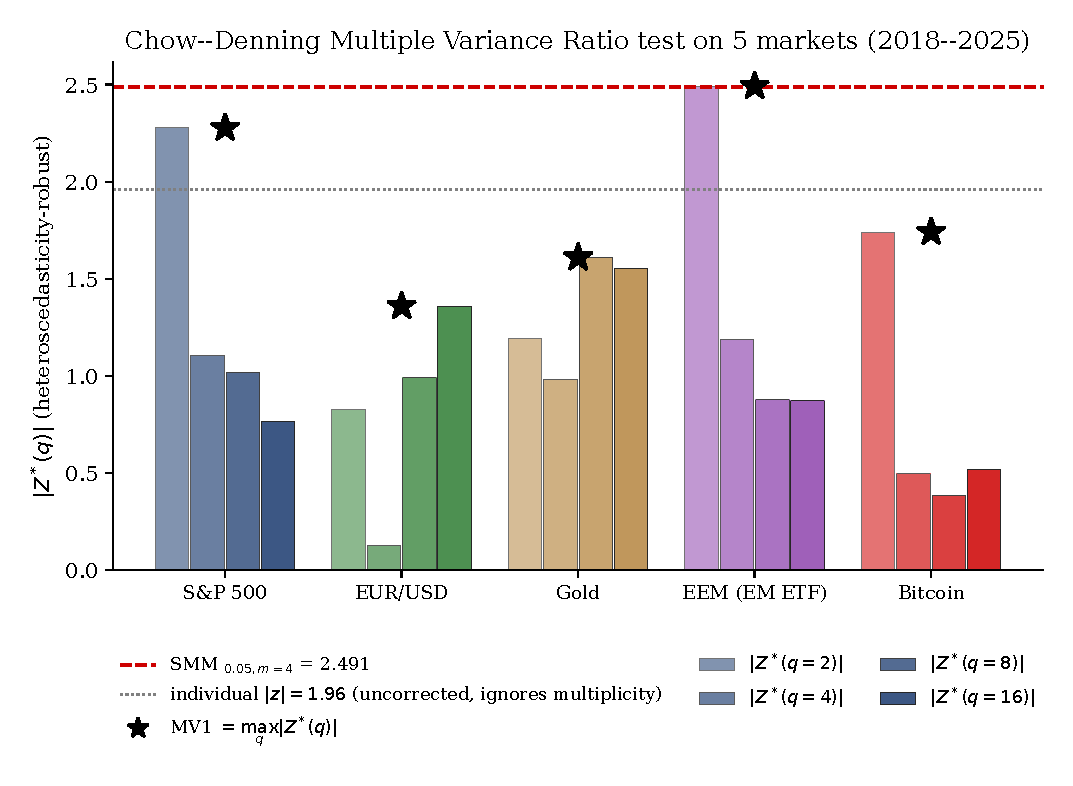
\includegraphics[width=\linewidth]{sfm_ch4_mv_test.pdf}
\end{column}
\begin{column}{0.37\textwidth}
\begin{itemize}\setlength{\itemsep}{0pt}
    \item \textbf{Configurare}
    \begin{itemize}\setlength{\itemsep}{0pt}
        \item $q \in \{2, 4, 8, 16\}$ (orizonturi diadice)
        \item $|Z^*(q)|$ heterosc-robust
    \end{itemize}
    \item \textbf{Praguri}
    \begin{itemize}\setlength{\itemsep}{0pt}
        \item Roșu: $\mathrm{SMM}_{0{,}05} = 2{,}491$ ($m=4$)
        \item Gri: $1{,}96$ (necorectat)
    \end{itemize}
    \item \textbf{Rezultate MV1}
    \begin{itemize}\setlength{\itemsep}{0pt}
        \item Nu respingem: S\&P ($2{,}28$), BTC ($1{,}74$), Gold ($1{,}61$), EUR/USD ($1{,}36$)
        \item \alert{Respinge}: EEM ($2{,}49 > 2{,}491$)
    \end{itemize}
    \item \textbf{Lecție}
    \begin{itemize}\setlength{\itemsep}{0pt}
        \item Pragul $1{,}96$ ar fi respins fals S\&P (la $q=2$)
    \end{itemize}
\end{itemize}
\end{column}
\end{columns}
\end{cminipage}
\vspace{0.05cm}
\quantlet{SFM\_ch4\_mv\_test}{https://colab.research.google.com/github/QuantLet/Stat_fin_markets/blob/master/Ch_04/SFM_ch4_mv_test/SFM_ch4_mv_test.ipynb}
\end{frame}

\begin{frame}[shrink=15]{Exercițiul 5: VR(5) cu test $Z$ --- enunț}
\begin{cminipage}{0.95\textwidth}
\begin{block}{Enunț}
\begin{itemize}\setlength{\itemsep}{0pt}
    \item Pe un activ se observă:
    \begin{itemize}\setlength{\itemsep}{0pt}
        \item $\hat\sigma^2_1 = 0{,}0001$ (varianța randamentelor zilnice)
        \item $\hat\sigma^2_5 = 0{,}000575$ (varianța randamentelor cumulate pe 5 zile)
        \item $T = 1.000$ observații zilnice
    \end{itemize}
\end{itemize}
\end{block}

\begin{itemize}\setlength{\itemsep}{0pt}
    \item \textbf{Cerințe}
    \begin{itemize}\setlength{\itemsep}{0pt}
        \item Calculați $VR(5) = \sigma^2_5 / (5 \cdot \sigma^2_1)$
        \item Calculați statistica $Z = (VR - 1)/\sqrt{2(q-1)/T}$
        \item Testați RW la $\alpha = 5\%$ ($z_{0{,}025} = 1{,}96$)
        \item Interpretați (momentum sau mean reversion)
    \end{itemize}
\end{itemize}
\end{cminipage}
\end{frame}

\begin{frame}[shrink=15]{Exercițiul 5: VR(5) cu test $Z$ --- rezolvare}
\begin{cminipage}{0.95\textwidth}
\begin{exampleblock}{Rezolvare}
\begin{itemize}\setlength{\itemsep}{0pt}
    \item \textbf{Calculul VR(5)}
    \begin{itemize}\setlength{\itemsep}{0pt}
        \item $VR(5) = 0{,}000575/(5 \cdot 0{,}0001) = 0{,}000575/0{,}0005 = \mathbf{1{,}15}$
    \end{itemize}
    \item \textbf{Statistica $Z$}
    \begin{itemize}\setlength{\itemsep}{0pt}
        \item $Z = (1{,}15 - 1)/\sqrt{2 \cdot 4/1000} = 0{,}15/\sqrt{0{,}008} = 0{,}15/0{,}0894$
        \item $Z \approx \mathbf{1{,}68}$
    \end{itemize}
    \item \textbf{Decizia}
    \begin{itemize}\setlength{\itemsep}{0pt}
        \item $|Z| = 1{,}68 < 1{,}96 \Rightarrow$ nu respingem RW la 5\%
        \item Marginal: $p \approx 0{,}09$ (semnificativ la 10\%)
    \end{itemize}
    \item \textbf{Interpretare}
    \begin{itemize}\setlength{\itemsep}{0pt}
        \item $VR > 1 \Rightarrow$ tendință de momentum
        \item Statistic nesemnificativ la 5\%
        \item Economic: pe termen de 5 zile, randamentele au ușoară persistență
    \end{itemize}
\end{itemize}
\end{exampleblock}
\end{cminipage}
\end{frame}

\begin{frame}[shrink=15]{Sinteză: testele de eficiență slabă}
\begin{cminipage}{0.95\textwidth}
\begin{block}{Ce am acoperit pentru EMH forma slabă}
\renewcommand{\arraystretch}{1.25}
\begin{center}
\footnotesize
\begin{tabular}{lll}
\toprule
\textbf{Test} & \textbf{Ce măsoară} & \textbf{Punct slab} \\
\midrule
ACF / autocorelație & Dependență liniară la fiecare lag $k$ & Doar lineară; fereastră fixă \\
Ljung--Box $Q(m)$ & Toate $\rho_1, \ldots, \rho_m$ \emph{simultan} & Sensibil la $m$, presupune momente finite \\
Runs test & Aleatorismul \emph{semnelor} & Ignoră magnitudinea \\
Variance ratio $VR(q)$ & Agregarea varianței pe orizontul $q$ & Sensibil la cozi grele și outliers \\
MV (Chow--Denning) & VR pe \emph{mai multe} orizonturi simultan & Necesită SMM, nu p-value direct \\
\bottomrule
\end{tabular}
\end{center}
\end{block}

\vspace{0.15cm}
\begin{alertblock}{Reguli practice}
\begin{itemize}\setlength{\itemsep}{0pt}
    \item Niciun test nu este complet --- folosiți $\geq 2$ teste complementare
    \item Întotdeauna verificați \emph{robustețea} la cozi grele și clustering volatilitate
    \item Distingeți \emph{semnificația statistică} de \emph{semnificația economică}
\end{itemize}
\end{alertblock}
\end{cminipage}
\end{frame}

%=============================================================================
% PARTEA V: COZI GRELE ȘI LIMITELE TESTELOR
%=============================================================================
\section{Partea V: Cozi grele și limitele testelor}

\begin{frame}[shrink=15]{Random Walk Normal vs Cauchy --- tabel comparativ}
\begin{cminipage}{0.95\textwidth}
\begin{block}{Proprietăți ale Random Walk-ului sub diferite distribuții}
\renewcommand{\arraystretch}{1.2}
\begin{center}
\footnotesize
\begin{tabular}{lcc}
\toprule
\textbf{Proprietate} & \textbf{Normal: $\varepsilon_t \sim \mathcal{N}(0,\sigma^2)$} & \textbf{Cauchy: $\varepsilon_t \sim C(0,\gamma)$} \\
\midrule
Media $\E[\varepsilon_t]$ & $0$ & Nu există \\
Varianța & $\sigma^2$ (finită) & $\infty$ \\
Proprietatea de martingal & Da & Nu (media nu există) \\
Central Limit Theorem (CLT) se aplică & Da ($\bar{r} \to \mathcal{N}$) & Nu ($\bar{r} \sim C(0,\gamma)$) \\
$\Var(P_T)$ după $T$ pași & $T\sigma^2$ & $\infty$ \\
Prob.\ randament $> 5\sigma$ & $\approx 3 \times 10^{-7}$ & $\approx 0{,}013$ \\
Ljung--Box valid & Da & Problematic (momente $\infty$) \\
Variance ratio valid & Da & Nu (varianța nedefinită) \\
\bottomrule
\end{tabular}
\end{center}
\end{block}

\vspace{0.1cm}
\begin{itemize}\setlength{\itemsep}{0pt}
    \item \textbf{Implicație:} Testele clasice de eficiență presupun momente finite
    \item Dacă randamentele au cozi grele ($\alpha < 2$), testele trebuie adaptate
\end{itemize}
\end{cminipage}
\end{frame}

\begin{frame}[shrink=15]{Analogie McCulloch cuantile $\sim$ Variance Ratio}
\begin{cminipage}{0.95\textwidth}
\begin{columns}[T]
\begin{column}{0.48\textwidth}
\begin{block}{McCulloch: cuantile $\to$ $\alpha$}
\begin{itemize}\setlength{\itemsep}{0pt}
    \item $v_\alpha = \frac{q_{0{,}95} - q_{0{,}05}}{q_{0{,}75} - q_{0{,}25}}$
    \item Măsoară \textit{greutatea cozilor}
    \item Normal: $v_\alpha \approx 2{,}44$
    \item Cauchy: $v_\alpha \approx 25{,}0$
    \item \textbf{Idee:} raportul de range-uri
\end{itemize}
\end{block}
\end{column}
\begin{column}{0.48\textwidth}
\begin{block}{Variance Ratio: varianțe $\to$ eficiență}
\begin{itemize}\setlength{\itemsep}{0pt}
    \item $VR(q) = \frac{\sigma^2(q)}{q \cdot \sigma^2(1)}$
    \item Măsoară \textit{dependența serială}
    \item Random walk: $VR(q) = 1$
    \item Mean reversion: $VR(q) < 1$
    \item \textbf{Idee:} raportul de varianțe
\end{itemize}
\end{block}
\end{column}
\end{columns}

\vspace{0.3cm}
\begin{itemize}\setlength{\itemsep}{0pt}
    \item \textbf{Analogie:} Ambele folosesc \textit{rapoarte} de statistici la \textit{scale diferite}
    \item McCulloch: scale spațiale (cuantile); VR: scale temporale (orizonturi)
    \item \textbf{Robustețe diferită:} McCulloch este \emph{robust la outliers} (cuantilele nu sunt afectate); VR \emph{nu este robust} --- folosește varianțe care explodează la cozi grele
    \item \textbf{Consecință:} dacă $\alpha < 2$ (cozi grele, varianță infinită), VR este distorsionat și trebuie folosite alternative (bootstrap, ranguri)
\end{itemize}
\end{cminipage}
\end{frame}

\begin{frame}[shrink=15]{Cozi grele și eficiența pieței}
\begin{cminipage}{0.95\textwidth}
\begin{columns}[T]
\begin{column}{0.48\textwidth}
\begin{block}{EMH presupune implicit cozi subțiri}
\begin{itemize}\setlength{\itemsep}{0pt}
    \item Testele clasice (Ljung--Box, VR) presupun $\Var(r_t) < \infty$
    \item Dacă $r_t \sim S(\alpha, \beta, \gamma, \delta)$ cu $\alpha < 2$:
    \begin{itemize}\setlength{\itemsep}{0pt}
        \item Varianța este infinită
        \item Ljung--Box $Q$ devine distorsionat
        \item VR nu converge la 1
    \end{itemize}
    \item \textbf{Paradox:} piața poate fi eficientă dar testele clasice o resping
\end{itemize}
\end{block}
\end{column}
\begin{column}{0.48\textwidth}
\begin{block}{Soluții robuste}
\begin{itemize}\setlength{\itemsep}{0pt}
    \item \textbf{VR cu corecție heteroscedastică} (Lo--MacKinlay)
    \item \textbf{Bootstrap:} fără presupuneri distribuționale
    \item \textbf{Teste bazate pe ranguri}
    \item \textbf{Teste bazate pe cuantile} (analogia McCulloch)
    \item \textbf{Sub-eșantionare} (subsampling): IC robuste fără momente
\end{itemize}
\end{block}
\end{column}
\end{columns}

\vspace{0.2cm}
\begin{alertblock}{Lecție cheie}
\begin{itemize}\setlength{\itemsep}{0pt}
    \item Înainte de a testa eficiența, verificați distribuția randamentelor
    \item Cozi grele pot invalida testele clasice (Ljung--Box, VR)
\end{itemize}
\end{alertblock}
\end{cminipage}
\end{frame}

%=============================================================================
% PARTEA VI: EVENT STUDY
%=============================================================================
\section{Partea VI: Event Study --- semi-tare}

\begin{frame}[shrink=15]{Metodologia event study}
\begin{cminipage}{0.95\textwidth}
\begin{block}{Etapele unui event study}
\begin{itemize}\setlength{\itemsep}{0pt}
    \item \textbf{Fereastra de estimare} $[-L, -M]$
    \begin{itemize}\setlength{\itemsep}{0pt}
        \item Estimăm modelul de piață: $r_{i,t} = \alpha + \beta r_{m,t} + \varepsilon_{i,t}$
    \end{itemize}
    \item \textbf{Fereastra de eveniment} $[-M+1, +T]$
    \begin{itemize}\setlength{\itemsep}{0pt}
        \item Calculăm AR (\textit{Abnormal Return}): $AR_{i,t} = r_{i,t} - (\hat\alpha + \hat\beta r_{m,t})$
    \end{itemize}
    \item \textbf{Cumulative AR}
    \begin{itemize}\setlength{\itemsep}{0pt}
        \item $CAR_i(t_1, t_2) = \sum_{t=t_1}^{t_2} AR_{i,t}$
        \item $\overline{CAR}(t_1, t_2) = \frac{1}{N}\sum_i CAR_i$
    \end{itemize}
    \item \textbf{Test de semnificație} --- două situații
    \begin{itemize}\setlength{\itemsep}{0pt}
        \item \emph{Un singur eveniment}, fereastra de lungime $L$:
        \;$\displaystyle t = \frac{CAR(\tau_1, \tau_2)}{\hat\sigma_\varepsilon \sqrt{L}}$
        \;\;($\hat\sigma_\varepsilon$ din fereastra de estimare)
        \item \emph{Agregat pe} $N$ evenimente:
        \;$\displaystyle t = \frac{\overline{CAR}(\tau_1, \tau_2)}{\hat\sigma_{CAR} / \sqrt{N}}$
        \;\;($\hat\sigma_{CAR}$ = std cross-secțional al $CAR_i$)
    \end{itemize}
\end{itemize}
\end{block}
\end{cminipage}
\end{frame}

\begin{frame}[shrink=15]{Event Study --- schema temporală}
\begin{cminipage}{0.95\textwidth}
\begin{center}
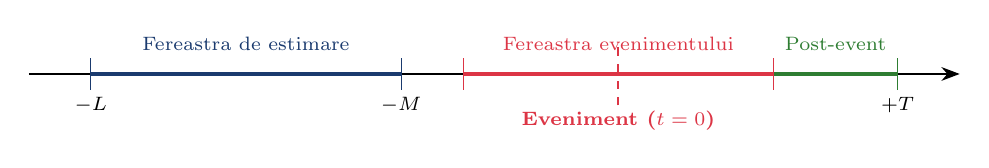
\begin{tikzpicture}[
    x=0.065\textwidth,
    every node/.style={font=\scriptsize}
]
% Timeline
\draw[-{Stealth}, thick] (-1,0) -- (14,0);
% Estimation window
\draw[MainBlue, very thick] (0,0) -- (5,0);
\draw[MainBlue] (0,-0.2) -- (0,0.2);
\draw[MainBlue] (5,-0.2) -- (5,0.2);
\node[above=5pt, MainBlue] at (2.5,0) {Fereastra de estimare};
\node[below=5pt] at (0,0) {$-L$};
\node[below=5pt] at (5,0) {$-M$};
% Event window
\draw[Crimson, very thick] (6,0) -- (11,0);
\draw[Crimson] (6,-0.2) -- (6,0.2);
\draw[Crimson] (11,-0.2) -- (11,0.2);
\node[above=5pt, Crimson] at (8.5,0) {Fereastra evenimentului};
% Event
\draw[Crimson, thick, dashed] (8.5,-0.4) -- (8.5,0.4);
\node[below=10pt, Crimson, font=\scriptsize\bfseries] at (8.5,0) {Eveniment ($t=0$)};
% Post-event
\draw[Forest, very thick] (11,0) -- (13,0);
\draw[Forest] (13,-0.2) -- (13,0.2);
\node[above=5pt, Forest] at (12,0) {Post-event};
\node[below=5pt] at (13,0) {$+T$};
\end{tikzpicture}
\end{center}

\vspace{0.2cm}
\renewcommand{\arraystretch}{1.2}
\begin{center}
\footnotesize
\begin{tabular}{llll}
\toprule
\textbf{Fereastră} & \textbf{Interval tipic} & \textbf{Scop} & \textbf{Calculăm} \\
\midrule
Estimare & $[-250, -11]$ & Parametrii modelului & $\hat\alpha_i, \hat\beta_i$ \\
Eveniment & $[-10, +10]$ & Detectarea reacției & $AR_{it}$, $CAR_i$ \\
Post-event & $[+11, +60]$ & Drift pe termen lung & $CAR$ cumulat \\
\bottomrule
\end{tabular}
\end{center}
\end{cminipage}
\end{frame}

\begin{frame}[shrink=15]{CAR: 3 scenarii + AAPL}
\begin{cminipage}{0.95\textwidth}
\begin{columns}[T]
\begin{column}{0.62\textwidth}
\centering
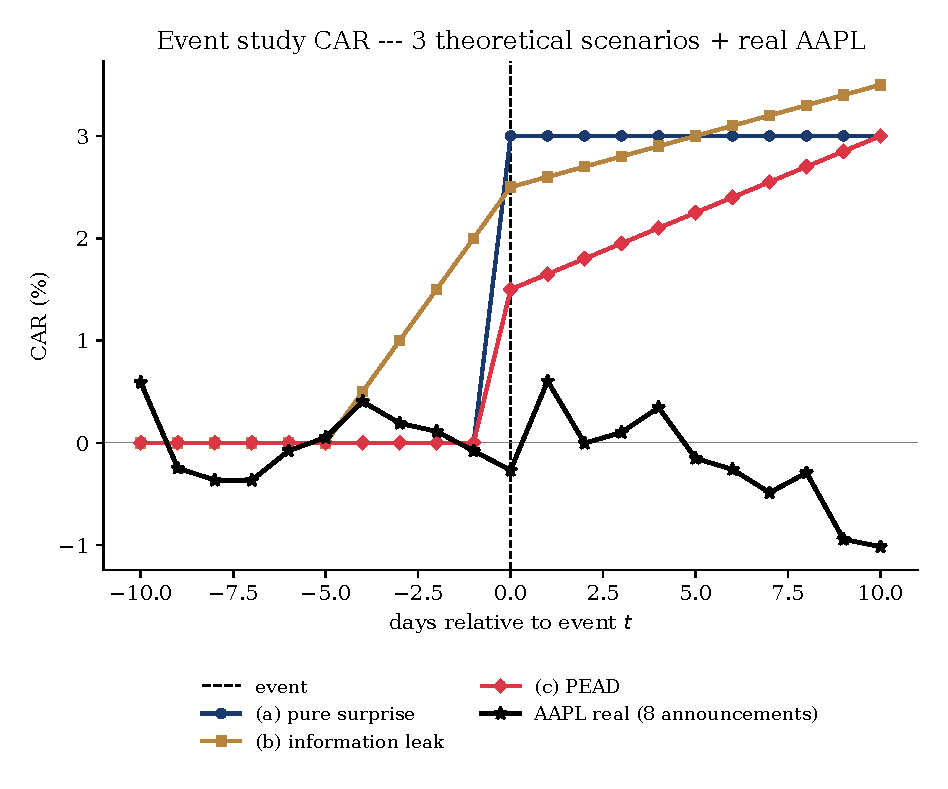
\includegraphics[width=0.95\linewidth,height=0.7\textheight,keepaspectratio]{sfm_ch4_car_scenarios.pdf}
\end{column}
\begin{column}{0.37\textwidth}
\footnotesize
\begin{itemize}\setlength{\itemsep}{0pt}
    \item \textbf{(a) Surpriză pură}
    \begin{itemize}\setlength{\itemsep}{0pt}
        \item Salt la $t=0$, EMH semi-tare ok
    \end{itemize}
    \item \textbf{(b) Leak}
    \begin{itemize}\setlength{\itemsep}{0pt}
        \item Drift pre-event, contra EMH tare
    \end{itemize}
    \item \textbf{(c) PEAD}
    \begin{itemize}\setlength{\itemsep}{0pt}
        \item Post-Earnings Announcement Drift
        \item Drift post-event, contra semi-tare
    \end{itemize}
    \item \textbf{AAPL (8 earnings reale)}
\end{itemize}
\end{column}
\end{columns}
\end{cminipage}
\vspace{0.05cm}
\quantlet{SFM\_ch4\_car\_scenarios}{https://colab.research.google.com/github/QuantLet/Stat_fin_markets/blob/master/Ch_04/SFM_ch4_car_scenarios/SFM_ch4_car_scenarios.ipynb}
\end{frame}

\begin{frame}[shrink=15]{Event study: CAR cu intervale de încredere 95\%}
\begin{cminipage}{0.95\textwidth}
\begin{columns}[T]
\begin{column}{0.6\textwidth}
\centering
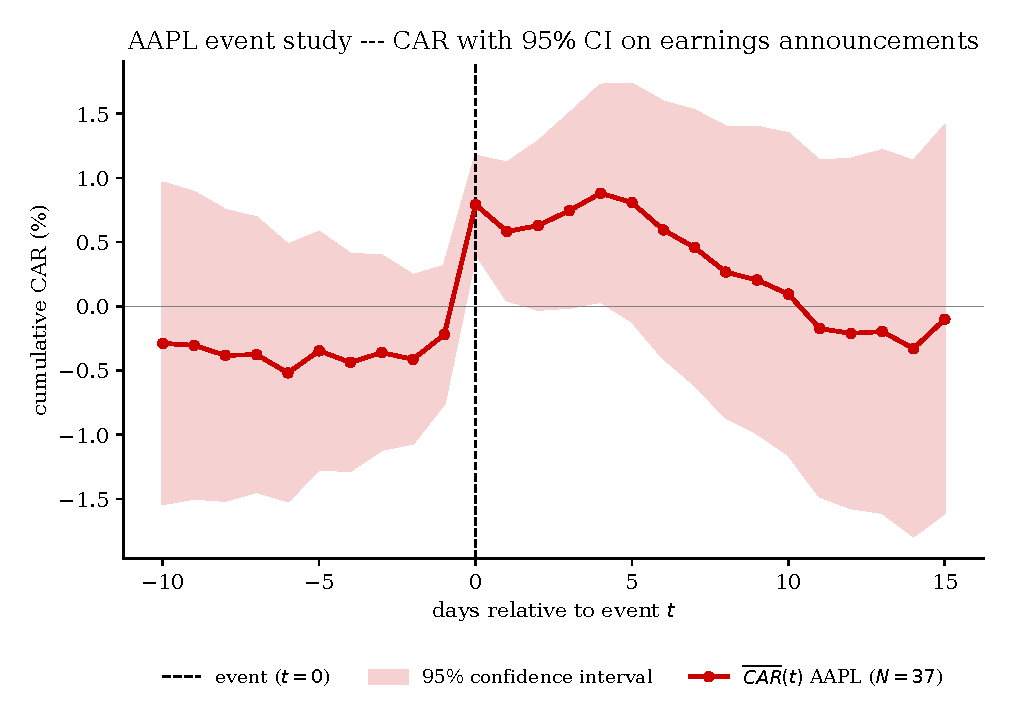
\includegraphics[width=\linewidth]{sfm_ch4_car_with_ci.pdf}
\end{column}
\begin{column}{0.37\textwidth}
\begin{itemize}\setlength{\itemsep}{0pt}
    \item \textbf{Date}
    \begin{itemize}\setlength{\itemsep}{0pt}
        \item AAPL + SPY (proxy piață), zilnic
        \item 37 anunțuri earnings 2015--2024
    \end{itemize}
    \item \textbf{Construcția IC pentru $\overline{CAR}$}
    \begin{itemize}\setlength{\itemsep}{0pt}
        \item $\displaystyle SE_t = \frac{\hat\sigma_\varepsilon \sqrt{|t|+1}}{\sqrt{N}}$
        \item $IC_{95\%} = \overline{CAR}_t \pm 1{,}96 \cdot SE_t$
    \end{itemize}
    \item \textbf{Citire grafică}
    \begin{itemize}\setlength{\itemsep}{0pt}
        \item Pre-event: IC conține $0$ $\Rightarrow$ fără leak
        \item La $t = 0$: salt în afara IC
        \item Post-event: drift (PEAD slabă)
    \end{itemize}
\end{itemize}
\end{column}
\end{columns}
\end{cminipage}
\vspace{0.05cm}
\quantlet{SFM\_ch4\_car\_with\_ci}{https://colab.research.google.com/github/QuantLet/Stat_fin_markets/blob/master/Ch_04/SFM_ch4_car_with_ci/SFM_ch4_car_with_ci.ipynb}
\end{frame}

\begin{frame}[shrink=15]{Șase studii AAPL individuale --- eterogenitate event-pe-event}
\begin{cminipage}{0.95\textwidth}
\begin{columns}[T]
\begin{column}{0.7\textwidth}
\centering
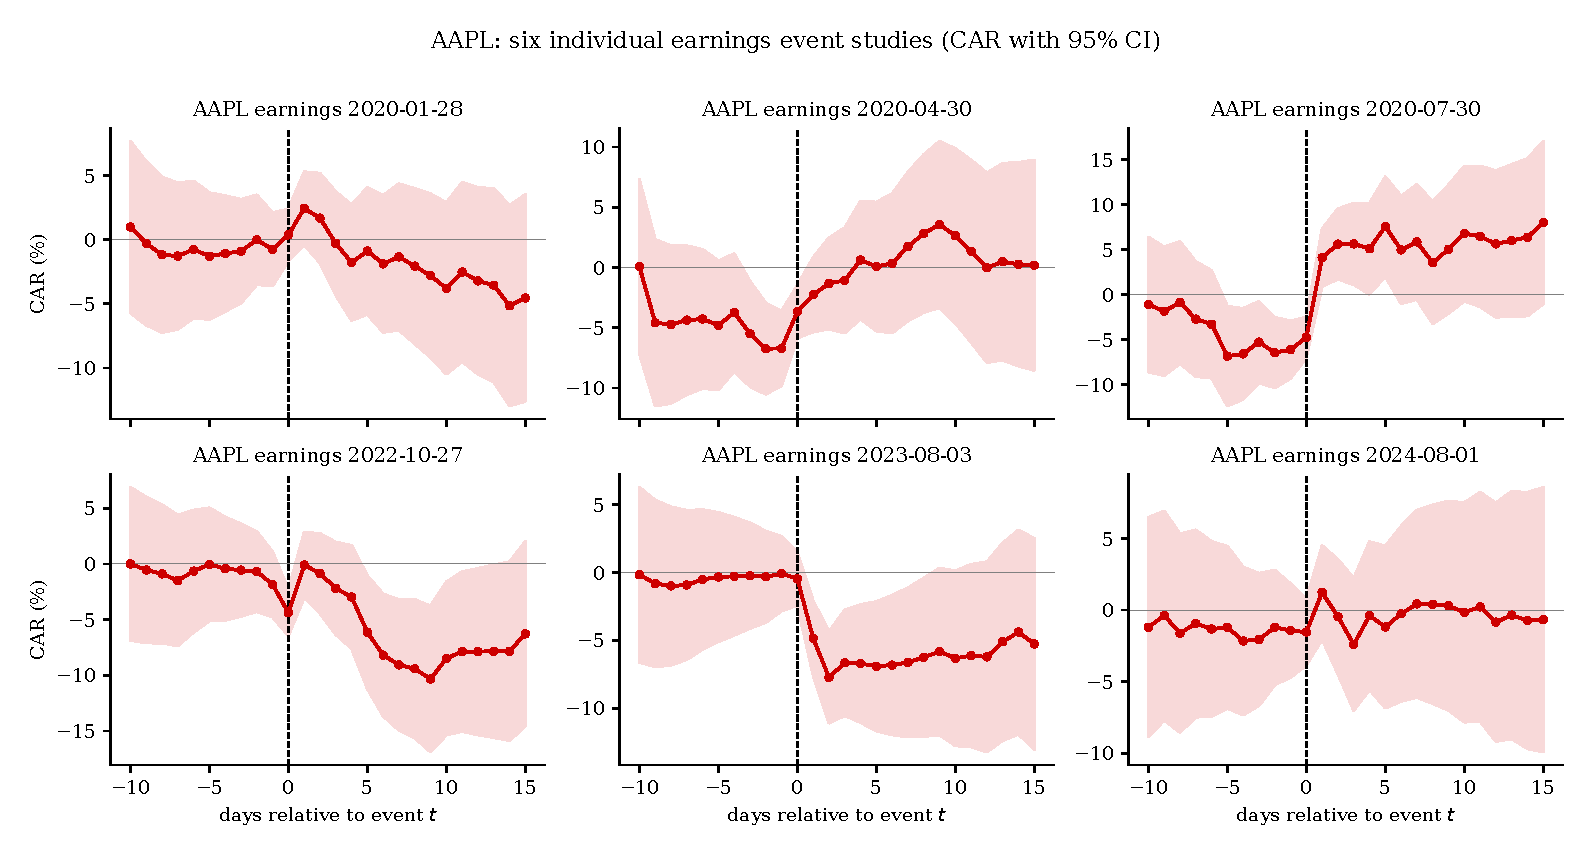
\includegraphics[width=\linewidth]{sfm_ch4_apple_events_grid.pdf}
\end{column}
\begin{column}{0.28\textwidth}
\footnotesize
\begin{itemize}\setlength{\itemsep}{0pt}
    \item \textbf{6 anunțuri AAPL}
    \begin{itemize}\setlength{\itemsep}{0pt}
        \item 2020 Q1, Q2, Q3
        \item 2022 Q4, 2023 Q3
        \item 2024 Q3 (AI)
    \end{itemize}
    \item \textbf{Forme CAR}
    \begin{itemize}\setlength{\itemsep}{0pt}
        \item Salt rapid
        \item Drift continuu
        \item Drift inversat
    \end{itemize}
    \item \textbf{Lecție}
    \begin{itemize}\setlength{\itemsep}{0pt}
        \item $\overline{CAR}$ ascunde eterogenitatea
        \item Raportați statistici per eveniment
    \end{itemize}
\end{itemize}
\end{column}
\end{columns}
\end{cminipage}
\vspace{0.05cm}
\quantlet{SFM\_ch4\_apple\_events\_grid}{https://colab.research.google.com/github/QuantLet/Stat_fin_markets/blob/master/Ch_04/SFM_ch4_apple_events_grid/SFM_ch4_apple_events_grid.ipynb}
\end{frame}

\begin{frame}[shrink=15]{Exercițiul 6: AR și CAR --- calcul tabular}
\begin{cminipage}{0.95\textwidth}
\begin{block}{Problemă}
\begin{itemize}\setlength{\itemsep}{0pt}
    \item O companie anunță rezultatele trimestriale la $t=0$. Din fereastra de estimare: $\hat\alpha = 0{,}001$, $\hat\beta = 1{,}2$, $\hat\sigma_\varepsilon = 0{,}015$. Calculați AR și CAR.
\end{itemize}
\end{block}

\begin{exampleblock}{Rezolvare}
\renewcommand{\arraystretch}{1.1}
\begin{center}
\footnotesize
\begin{tabular}{ccccc}
\toprule
$t$ & $R_{it}$ & $R_{mt}$ & $\E[R_{it}] = 0{,}001 + 1{,}2 R_{mt}$ & $AR_{it}$ \\
\midrule
$-2$ & 0{,}005 & 0{,}003 & 0{,}0046 & 0{,}0004 \\
$-1$ & 0{,}012 & 0{,}002 & 0{,}0034 & \textcolor{Forest}{\textbf{0{,}0086}} \\
$0$ & 0{,}035 & 0{,}005 & 0{,}0070 & \textcolor{Forest}{\textbf{0{,}0280}} \\
$+1$ & 0{,}008 & 0{,}004 & 0{,}0058 & 0{,}0022 \\
$+2$ & $-0{,}002$ & $-0{,}001$ & $-0{,}0002$ & $-0{,}0018$ \\
\bottomrule
\end{tabular}
\end{center}

\small
\begin{itemize}\setlength{\itemsep}{0pt}
    \item $CAR(-1, +1) = 0{,}0086 + 0{,}0280 + 0{,}0022 = \mathbf{0{,}0388}$ (3{,}88\%)
    \item $t_{\text{CAR}} = 0{,}0388 / (0{,}015 / \sqrt{3}) = 0{,}0388 / 0{,}00866 = \mathbf{4{,}48}$
    \item $|t| = 4{,}48 > 1{,}96$ $\Rightarrow$ \textcolor{Forest}{\textbf{CAR semnificativ pozitiv}} --- piața reacționează la anunț
\end{itemize}
\end{exampleblock}
\end{cminipage}
\end{frame}

\begin{frame}[shrink=15]{Exercițiul 6 cont.: Interpretare scenarii AR}
\begin{cminipage}{0.95\textwidth}
\begin{columns}[T]
\begin{column}{0.48\textwidth}
\begin{block}{Piață eficientă (semi-tare)}
\begin{itemize}\setlength{\itemsep}{0pt}
    \item Tot $AR$ concentrat la $t=0$
    \item $AR_{-1} \approx 0$ (fără anticipare)
    \item $AR_{+1}, AR_{+2} \approx 0$ (absorbție rapidă)
    \item CAR: salt la $t=0$, apoi plat
\end{itemize}
\end{block}
\end{column}
\begin{column}{0.48\textwidth}
\begin{block}{Ce observăm în datele noastre}
\begin{itemize}\setlength{\itemsep}{0pt}
    \item $AR_{-1} = 0{,}86\%$ --- \textcolor{Crimson}{posibil insider trading}
    \item $AR_0 = 2{,}80\%$ --- reacție principală
    \item $AR_{+1} = 0{,}22\%$ --- absorbție lentă
    \item \textbf{Concluzie:} Evidență contra eficienței semi-tari
\end{itemize}
\end{block}
\end{column}
\end{columns}

\vspace{0.3cm}
\renewcommand{\arraystretch}{1.2}
\begin{center}
\footnotesize
\begin{tabular}{lccc}
\toprule
\textbf{Scenariu} & \textbf{$AR$ pre-event} & \textbf{$AR$ la $t=0$} & \textbf{$AR$ post-event} \\
\midrule
Eficient & $\approx 0$ & Mare & $\approx 0$ \\
Insider trading & Semnificativ & Mare & $\approx 0$ \\
Reacție lentă (PEAD) & $\approx 0$ & Mic & Semnificativ \\
Suprareacție & $\approx 0$ & Foarte mare & Negativ (reversal) \\
\bottomrule
\end{tabular}
\end{center}
\end{cminipage}
\end{frame}

\begin{frame}[shrink=15]{Exercițiul 7: CAR cu surpriză pură --- enunț}
\begin{cminipage}{0.95\textwidth}
\begin{block}{Enunț}
\begin{itemize}\setlength{\itemsep}{0pt}
    \item Anunț neașteptat la $t = 0$; fereastra $[-2, +3]$:
    \begin{itemize}\setlength{\itemsep}{0pt}
        \item $AR$ (\%): $-0{,}2$; $0{,}1$; $\mathbf{2{,}8}$; $0{,}6$; $-0{,}1$; $0{,}2$ (pentru $t = -2, \ldots, +3$)
        \item Deviația std.\ pe fereastra de estimare: $\hat\sigma_{AR} = 1{,}3\%$
    \end{itemize}
\end{itemize}
\end{block}

\begin{itemize}\setlength{\itemsep}{0pt}
    \item \textbf{Cerințe}
    \begin{itemize}\setlength{\itemsep}{0pt}
        \item Calculați CAR$[-2, +3]$
        \item Testați $H_0: CAR = 0$ cu $t = CAR/(\hat\sigma_{AR}\sqrt{L})$
        \item Este evenimentul surpriză pură, leak sau PEAD?
        \item Concluzia pentru EMH semi-tare
    \end{itemize}
\end{itemize}
\end{cminipage}
\end{frame}

\begin{frame}[shrink=15]{Exercițiul 7: CAR cu surpriză pură --- rezolvare}
\begin{cminipage}{0.95\textwidth}
\begin{exampleblock}{Rezolvare}
\begin{itemize}\setlength{\itemsep}{0pt}
    \item \textbf{CAR}
    \begin{itemize}\setlength{\itemsep}{0pt}
        \item $CAR[-2, +3] = -0{,}2 + 0{,}1 + 2{,}8 + 0{,}6 - 0{,}1 + 0{,}2 = \mathbf{3{,}4\%}$
    \end{itemize}
    \item \textbf{Testul $t$}
    \begin{itemize}\setlength{\itemsep}{0pt}
        \item $L = 6$; $t = 3{,}4/(1{,}3 \cdot \sqrt{6}) = 3{,}4/3{,}18 \approx \mathbf{1{,}07}$
        \item $|t| < 1{,}96 \Rightarrow$ nu respingem pe eveniment individual
        \item Agregat pe $N$ evenimente crește puterea testului
    \end{itemize}
    \item \textbf{Diagnostic}
    \begin{itemize}\setlength{\itemsep}{0pt}
        \item $AR_{-2}, AR_{-1}$ foarte mici $\Rightarrow$ \textbf{nu există leak}
        \item Salt $+2{,}8\%$ la $t=0$, $+0{,}6\%$ la $t=+1$ $\Rightarrow$ \textbf{surpriză pură}
        \item Ajustare rapidă (1--2 zile)
    \end{itemize}
    \item \textbf{Concluzie EMH semi-tare}
    \begin{itemize}\setlength{\itemsep}{0pt}
        \item Ajustare rapidă la info publică $\Rightarrow$ compatibil cu EMH semi-tare
    \end{itemize}
\end{itemize}
\end{exampleblock}
\end{cminipage}
\end{frame}

\begin{frame}[shrink=15]{Comparație: Teste pentru formele EMH}
\begin{cminipage}{0.95\textwidth}
\renewcommand{\arraystretch}{1.2}
\begin{center}
\footnotesize
\begin{tabular}{llll}
\toprule
\textbf{Forma EMH} & \textbf{Teste} & \textbf{$H_0$} & \textbf{Rezultate tipice} \\
\midrule
\multirow{3}{*}{Slabă} & Autocorelație / Ljung--Box & $\rho_k = 0, \forall k$ & Mici dar semnificative \\
 & Runs test & Secvență aleatoare & Ușoară alternare \\
 & Variance ratio (cu IC) & $VR(q) = 1$ & $VR < 1$ pe termen scurt \\
\midrule
\multirow{2}{*}{Semi-tare} & Event study & $CAR = 0$ & CAR $\neq 0$ pre/post \\
 & Anomalii calendaristice & Fără efect sezonier & Efect ianuarie, luni \\
\midrule
\multirow{2}{*}{Tare} & Performanța insiders & Fără exces retur & Exces semnificativ \\
 & Fonduri mutual & $\alpha_{\text{Jensen}} = 0$ & $\alpha \approx 0$ (net fees) \\
\bottomrule
\end{tabular}
\end{center}

\vspace{0.2cm}
\begin{itemize}\setlength{\itemsep}{0pt}
    \item \textbf{Rezultat general:} Forma slabă --- în mare parte confirmată; semi-tare --- evidență mixtă; tare --- respinsă
    \item Eficiența variază în timp (Andrew Lo, 2004: Adaptive Markets Hypothesis)
\end{itemize}
\end{cminipage}
\end{frame}

%=============================================================================
% PARTEA VII: AMH + ANOMALII
%=============================================================================
\section{Partea VII: AMH și anomalii}

\begin{frame}[shrink=15]{Adaptive Markets Hypothesis (Lo, 2004)}
\begin{cminipage}{0.95\textwidth}
\begin{columns}[T]
\begin{column}{0.46\textwidth}
\begin{block}{Idee centrală}
\begin{itemize}\setlength{\itemsep}{0pt}
    \item Eficiența \textbf{nu este o proprietate fixă} a piețelor
    \item Variază în timp odată cu condițiile de mediu (volatilitate, lichiditate, panică)
    \item EMH = caz limită al AMH, când piața este în echilibru
\end{itemize}
\end{block}

\begin{block}{Predicții AMH}
\begin{itemize}\setlength{\itemsep}{0pt}
    \item În crize: $|\hat\rho_1|$ crește, $p$-value Ljung--Box scade $\Rightarrow$ ineficiență
    \item În perioade calme: $\hat\rho_1$ aproape de $0$, $p$-value-uri Ljung--Box mari ($p \gg 0{,}05$) $\Rightarrow$ nu respingem EMH slabă
    \item Anomaliile apar și dispar (Schwert, 2003)
\end{itemize}
\end{block}
\end{column}
\begin{column}{0.5\textwidth}
\centering
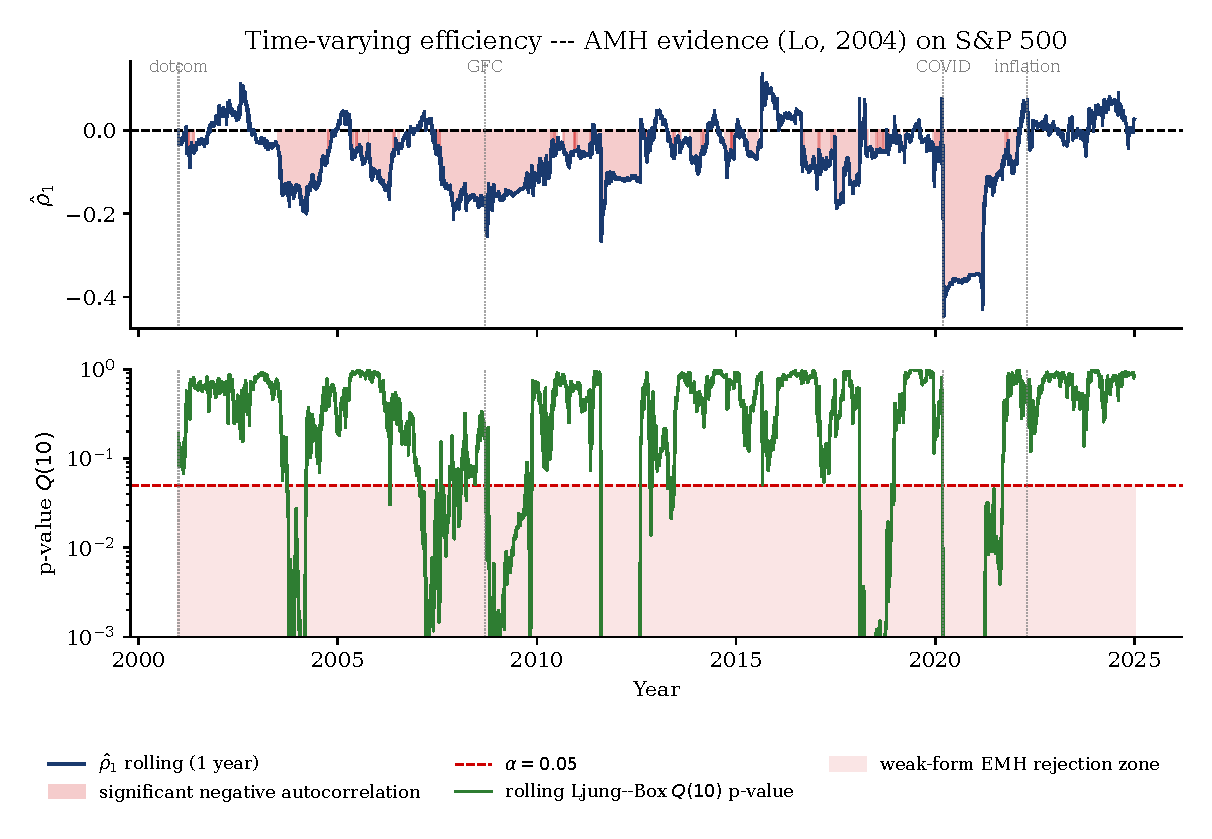
\includegraphics[width=\linewidth]{sfm_ch4_amh_rolling.pdf}
\end{column}
\end{columns}
\end{cminipage}
\vspace{0.05cm}
\quantlet{SFM\_ch4\_amh\_rolling}{https://colab.research.google.com/github/QuantLet/Stat_fin_markets/blob/master/Ch_04/SFM_ch4_amh_rolling/SFM_ch4_amh_rolling.ipynb}
\end{frame}

\begin{frame}[shrink=15]{Anomalii calendaristice}
\begin{cminipage}{0.95\textwidth}
\begin{block}{Exercițiu: Anomalia de luni (Monday effect)}
\begin{itemize}\setlength{\itemsep}{0pt}
    \item Randamente medii pe zile (date istorice, S\&P 500):
\end{itemize}
\renewcommand{\arraystretch}{1.2}
\begin{center}
\begin{tabular}{lccccc}
\toprule
 & Luni & Marți & Miercuri & Joi & Vineri \\
\midrule
$\bar{r}$ (\%) & $-0{,}08$ & 0{,}02 & 0{,}05 & 0{,}04 & 0{,}06 \\
$t$-stat & $-2{,}10$ & 0{,}55 & 1{,}32 & 1{,}05 & 1{,}58 \\
\bottomrule
\end{tabular}
\end{center}
\end{block}

\vspace{0.2cm}
\begin{itemize}\setlength{\itemsep}{0pt}
    \item Luni: randament negativ semnificativ ($t = -2{,}10$, $p < 0{,}05$)
    \item \textbf{Explicații posibile:} efectul weekend-ului, investitori instituționali, settlement
    \item \textbf{Contra-argument:} anomalia a \textit{dispărut} după publicare (Schwert, 2003)
    \item Alte anomalii: \textbf{efect ianuarie}, efect turn-of-month, efect Halloween
    \item \textbf{AMH (Lo, 2004):} Anomaliile apar și dispar pe măsură ce piața se adaptează
\end{itemize}
\end{cminipage}
\end{frame}

\begin{frame}[shrink=15]{Semnificație statistică vs semnificație economică}
\begin{cminipage}{0.95\textwidth}
\begin{alertblock}{Mesaj cheie}
\centering
\textbf{Predictibilitate statistică $\neq$ profit net tranzacționabil}\\[0.1cm]
\footnotesize
$\displaystyle \text{respinge } H_0 \;\not\Rightarrow\; \text{strategie profitabilă net de costuri}$
\end{alertblock}

\vspace{0.1cm}
\begin{columns}[T]
\begin{column}{0.48\textwidth}
\begin{block}{Fricțiuni care erodează profitul}
\footnotesize
\begin{itemize}\setlength{\itemsep}{0pt}
    \item \textbf{Costuri directe}
    \begin{itemize}\setlength{\itemsep}{0pt}
        \item Comisioane, bid--ask spread, slippage, taxe
    \end{itemize}
    \item \textbf{Limite practice}
    \begin{itemize}\setlength{\itemsep}{0pt}
        \item Capacitate limitată, risc de model, data snooping
    \end{itemize}
\end{itemize}
\end{block}
\end{column}
\begin{column}{0.48\textwidth}
\begin{exampleblock}{Exemplu: $\hat\rho_1 = -0{,}05$ (lag 1, $T = 6000$)}
\footnotesize
\begin{itemize}\setlength{\itemsep}{0pt}
    \item \textbf{Statistic}
    \begin{itemize}\setlength{\itemsep}{0pt}
        \item $z = \sqrt{T}\hat\rho_1 \approx 3{,}87$ $\Rightarrow$ respins la 5\%
    \end{itemize}
    \item \textbf{Economic}
    \begin{itemize}\setlength{\itemsep}{0pt}
        \item Brut $\sim 0{,}001\%$/zi vs costuri $\sim 0{,}05\%$/tranzacție
        \item Profit net $< 0$ $\Rightarrow$ eficient net
    \end{itemize}
\end{itemize}
\end{exampleblock}
\end{column}
\end{columns}

\vspace{0.05cm}
\begin{alertblock}{Pedersen (2015): ,,Efficiently inefficient''}
\footnotesize
\begin{itemize}\setlength{\itemsep}{0pt}
    \item Eficiente încât majoritatea nu le pot bate, cu fricțiuni încât traderii sofisticați extrag profit din anomalii temporare
\end{itemize}
\end{alertblock}
\end{cminipage}
\end{frame}

%=============================================================================
% PARTEA VIII: STRATEGII, COSTURI, SPIVA
%=============================================================================
\section{Partea VIII: Strategii, costuri, SPIVA}

\begin{frame}[shrink=15]{MA crossover: strategie clasică de trading}
\begin{cminipage}{0.95\textwidth}
\begin{block}{Regula Brock--Lakonishok--LeBaron (1992)}
\begin{itemize}\setlength{\itemsep}{0pt}
    \item Medie mobilă (MA, \textit{Moving Average}): $\text{MA}_t(k) = \frac{1}{k}\sum P_{t-i}$
    \item Cumpără când MA(50) $>$ MA(200) (Golden Cross)
    \item Vinde când MA(50) $<$ MA(200) (Death Cross)
    \item Ideea: exploatarea momentum-ului pe termen lung
\end{itemize}
\end{block}

\begin{alertblock}{Concluzie empirică}
\begin{itemize}\setlength{\itemsep}{0pt}
    \item Profitabilă pe date \textbf{pre-1990}
    \begin{itemize}\setlength{\itemsep}{0pt}
        \item BLL (1992) raportează excess return $\sim 3\%$/an
    \end{itemize}
    \item Dispare \textbf{post-1990}
    \begin{itemize}\setlength{\itemsep}{0pt}
        \item Piața se adaptează (consistent cu AMH)
        \item Costurile de tranzacție elimină profitul rămas
    \end{itemize}
\end{itemize}
\end{alertblock}
\end{cminipage}
\end{frame}

\begin{frame}[shrink=15]{Exemplu: MA(50)/MA(200) pe S\&P 500 (2010--2024)}
\begin{cminipage}{0.95\textwidth}
\centering
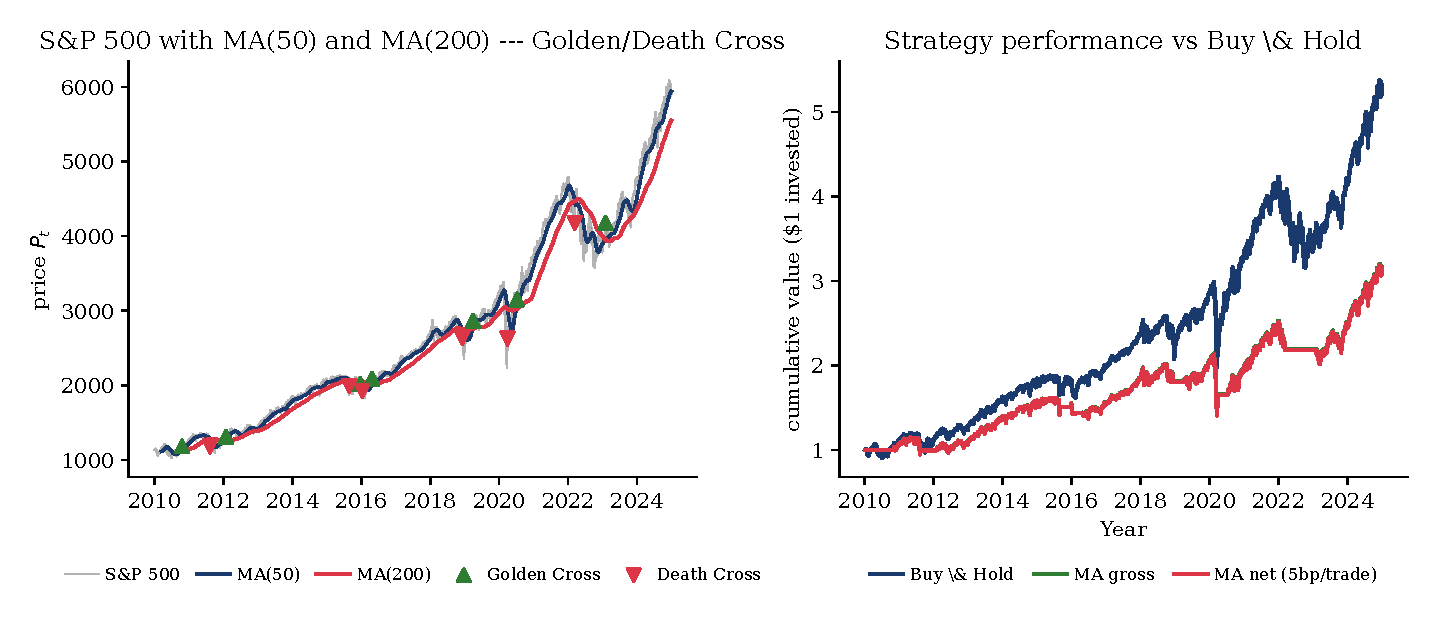
\includegraphics[width=\linewidth]{sfm_ch4_ma_crossover.pdf}
\end{cminipage}
\vspace{0.05cm}
\quantlet{SFM\_ch4\_ma\_crossover}{https://colab.research.google.com/github/QuantLet/Stat_fin_markets/blob/master/Ch_04/SFM_ch4_ma_crossover/SFM_ch4_ma_crossover.ipynb}
\end{frame}

\begin{frame}[shrink=15]{MA crossover: rezultate 2010--2024}
\begin{cminipage}{0.95\textwidth}
\begin{block}{Backtest pe 15 ani, S\&P 500, cu și fără costuri}
\begin{itemize}\setlength{\itemsep}{0pt}
    \item Buy \& Hold
    \begin{itemize}\setlength{\itemsep}{0pt}
        \item CAGR $= 11{,}65\%$; $\hat\sigma = 17{,}28\%$; Sharpe $= 0{,}56$
    \end{itemize}
    \item MA crossover \textbf{brut}
    \begin{itemize}\setlength{\itemsep}{0pt}
        \item CAGR $= 7{,}86\%$; $\hat\sigma = 13{,}73\%$; Sharpe $= 0{,}43$
        \item 13 tranzacții în 15 ani; $\sim 85\%$ timp în piață
    \end{itemize}
    \item MA crossover \textbf{net} (0{,}05\%/tranzacție)
    \begin{itemize}\setlength{\itemsep}{0pt}
        \item CAGR $= 7{,}81\%$; Sharpe $= 0{,}42$
    \end{itemize}
\end{itemize}
\end{block}

\begin{alertblock}{Verdict}
\begin{itemize}\setlength{\itemsep}{0pt}
    \item MA reduce $\sigma$ de la $17{,}3\%$ la $13{,}7\%$
    \item Dar pierde $\sim 3{,}8$pp de randament
    \item Sharpe B\&H ($0{,}56$) $>$ Sharpe MA ($0{,}42$)
    \item MA \textbf{nu} adaugă valoare ajustată la risc
    \item Consistent cu EMH slabă post-1990
\end{itemize}
\end{alertblock}
\end{cminipage}
\end{frame}

\begin{frame}[shrink=15]{MA crossover pre vs post 1990 --- evidență AMH}
\begin{cminipage}{0.95\textwidth}
\begin{columns}[T]
\begin{column}{0.6\textwidth}
\centering
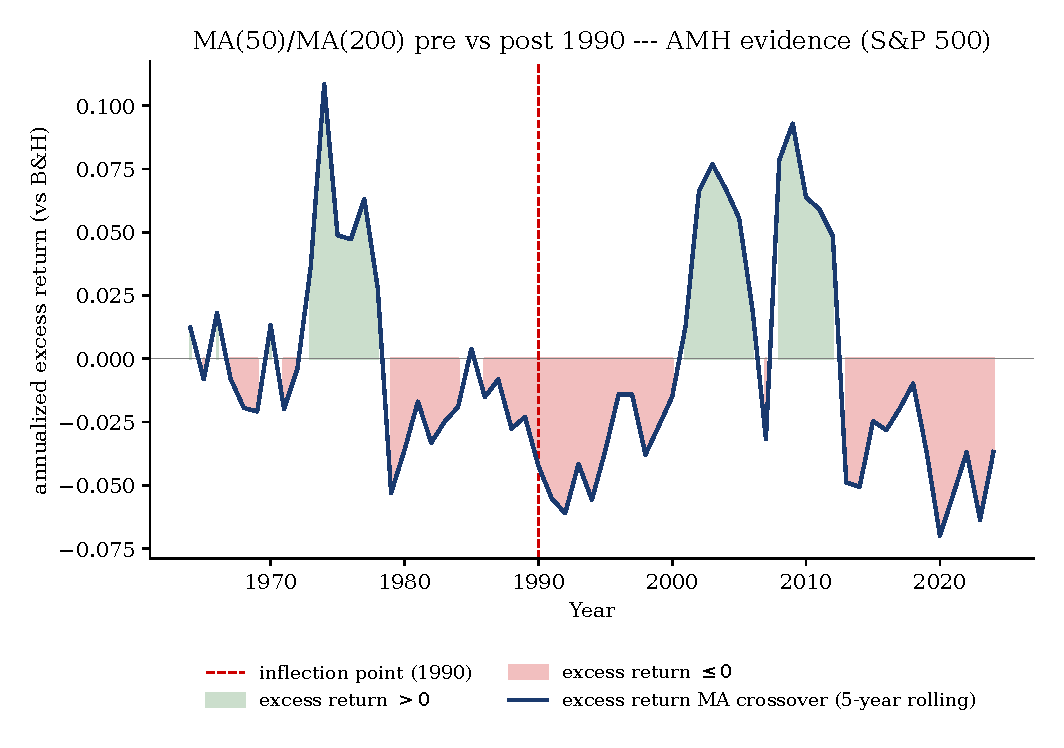
\includegraphics[width=\linewidth]{sfm_ch4_ma_pre_post.pdf}
\end{column}
\begin{column}{0.37\textwidth}
\begin{itemize}\setlength{\itemsep}{0pt}
    \item \textbf{Date:} S\&P 500 zilnic 1960--2024 (yfinance)
    \item \textbf{Pre-1990} (Brock, Lakonishok \& LeBaron, 1992)
    \begin{itemize}\setlength{\itemsep}{0pt}
        \item Excess return $\approx +3\%$/an
        \item Strategia bate Buy \& Hold
    \end{itemize}
    \item \textbf{Post-1990}
    \begin{itemize}\setlength{\itemsep}{0pt}
        \item Excess return oscilează în jur de $0$
        \item În medie ușor negativ după costuri
    \end{itemize}
    \item \textbf{De ce dispare?}
    \begin{itemize}\setlength{\itemsep}{0pt}
        \item Publicarea $\Rightarrow$ tranzacționare algoritmică
        \item Anomalia este \textit{arbitrată} (Schwert, 2003)
    \end{itemize}
\end{itemize}
\end{column}
\end{columns}
\end{cminipage}
\vspace{0.05cm}
\quantlet{SFM\_ch4\_ma\_pre\_post}{https://colab.research.google.com/github/QuantLet/Stat_fin_markets/blob/master/Ch_04/SFM_ch4_ma_pre_post/SFM_ch4_ma_pre_post.ipynb}
\end{frame}

\begin{frame}[shrink=15]{SPIVA: Active vs Passive (SPIVA Scorecard, 2024)}
\begin{cminipage}{0.95\textwidth}
\begin{columns}[T]
\begin{column}{0.58\textwidth}
\centering
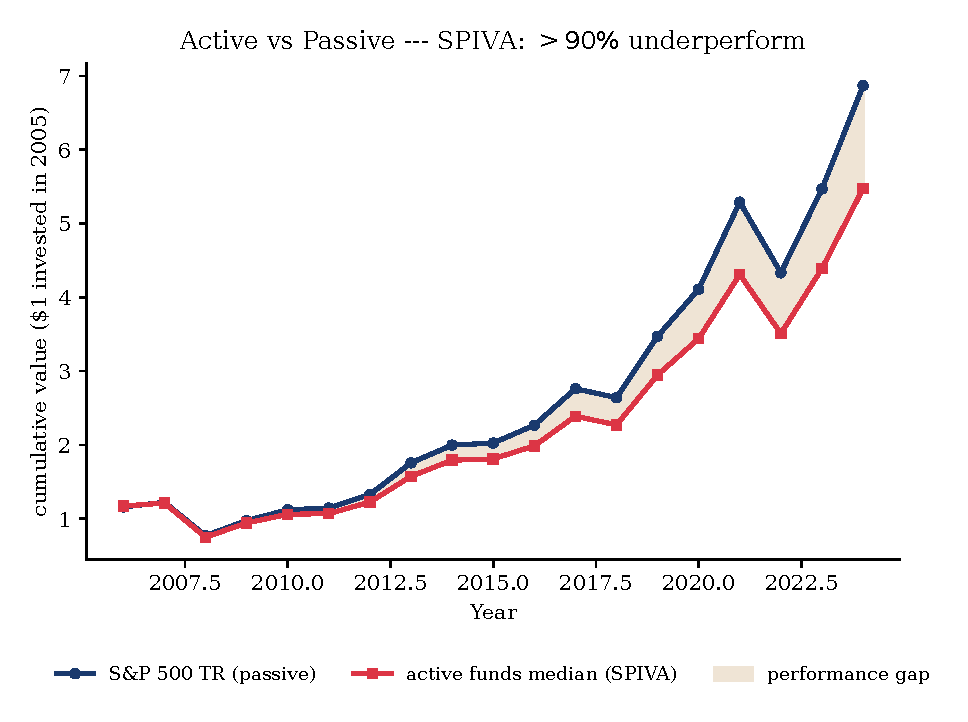
\includegraphics[width=\linewidth]{sfm_ch4_active_passive.pdf}
\end{column}
\begin{column}{0.4\textwidth}
\begin{itemize}\setlength{\itemsep}{0pt}
    \item Fapta empirică dominantă (large-cap, 15 ani)
    \begin{itemize}\setlength{\itemsep}{0pt}
        \item $> 90\%$ din fondurile active subperformează S\&P 500
        \item Gap cumulativ în favoarea indicelui pasiv
    \end{itemize}
    \item Cauze
    \begin{itemize}\setlength{\itemsep}{0pt}
        \item Comisioane $\sim 1\%$/an
        \item Cost tranzacționare și slippage
        \item Competiție între manageri informați
    \end{itemize}
    \item Consecință
    \begin{itemize}\setlength{\itemsep}{0pt}
        \item Fondurile index pasive dominante
        \item Argument puternic pentru EMH
    \end{itemize}
    \item \footnotesize\emph{Source: S\&P Dow Jones Indices, SPIVA U.S. Scorecard 2024}
\end{itemize}
\end{column}
\end{columns}
\end{cminipage}
\vspace{0.05cm}
\quantlet{SFM\_ch4\_active\_passive}{https://colab.research.google.com/github/QuantLet/Stat_fin_markets/blob/master/Ch_04/SFM_ch4_active_passive/SFM_ch4_active_passive.ipynb}
\end{frame}

\begin{frame}[shrink=15]{Bule și prăbușiri --- pattern-uri comparative}
\begin{cminipage}{0.95\textwidth}
\begin{columns}[T]
\begin{column}{0.58\textwidth}
\centering
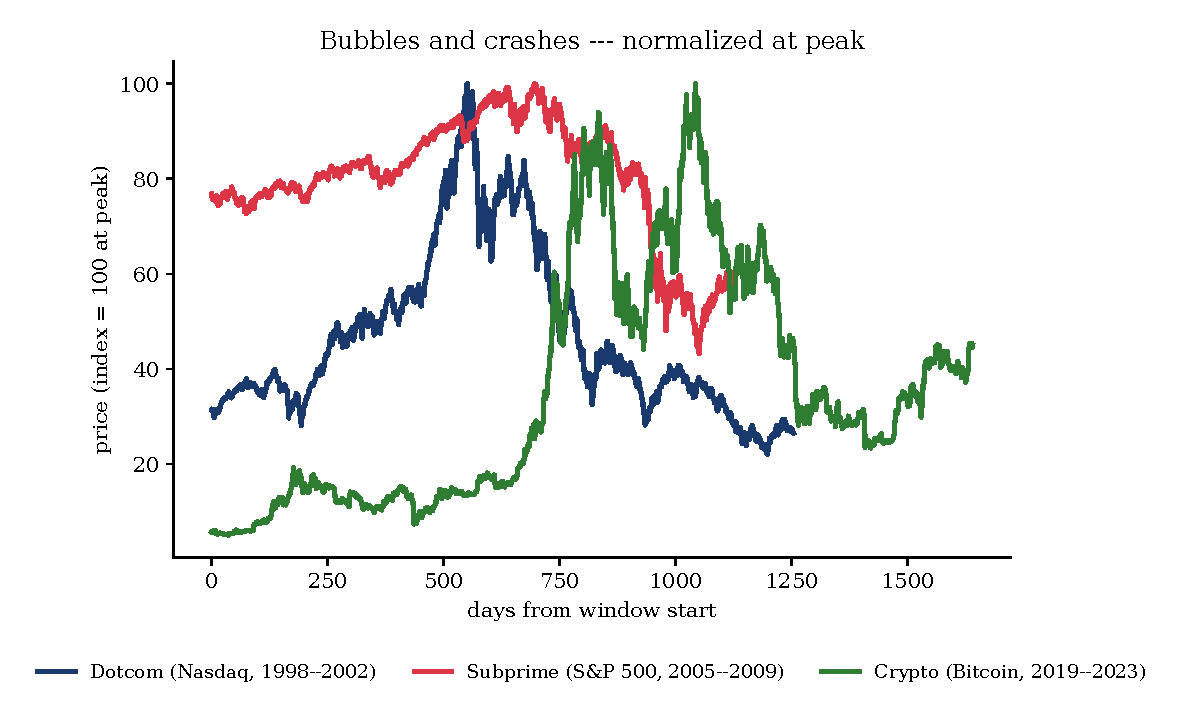
\includegraphics[width=\linewidth]{sfm_ch4_bubbles.pdf}
\end{column}
\begin{column}{0.4\textwidth}
\begin{itemize}\setlength{\itemsep}{0pt}
    \item Pattern universal
    \begin{itemize}\setlength{\itemsep}{0pt}
        \item Creștere exponențială înainte de vârf
        \item Vârf abrupt, urmat de cădere
        \item Asimetrie: urcăm lent, cădem rapid
    \end{itemize}
    \item Trei exemple
    \begin{itemize}\setlength{\itemsep}{0pt}
        \item Dotcom (Nasdaq, 2000)
        \item Subprime (S\&P 500, 2007--2008)
        \item Crypto (Bitcoin, 2021)
    \end{itemize}
    \item Lecția pentru EMH
    \begin{itemize}\setlength{\itemsep}{0pt}
        \item Bulele persistă în ciuda testelor
        \item Arbitrajul este costisitor și riscant
    \end{itemize}
\end{itemize}
\end{column}
\end{columns}
\end{cminipage}
\vspace{0.05cm}
\quantlet{SFM\_ch4\_bubbles}{https://colab.research.google.com/github/QuantLet/Stat_fin_markets/blob/master/Ch_04/SFM_ch4_bubbles/SFM_ch4_bubbles.ipynb}
\end{frame}

%=============================================================================
% PARTEA IX: STUDII DE CAZ
%=============================================================================
\section{Partea IX: Studii de caz}

\begin{frame}[shrink=15]{Studiu de caz 1: Comparație cross-asset (2020--2025)}
\begin{cminipage}{0.95\textwidth}
\begin{columns}[T]
\begin{column}{0.66\textwidth}
\centering
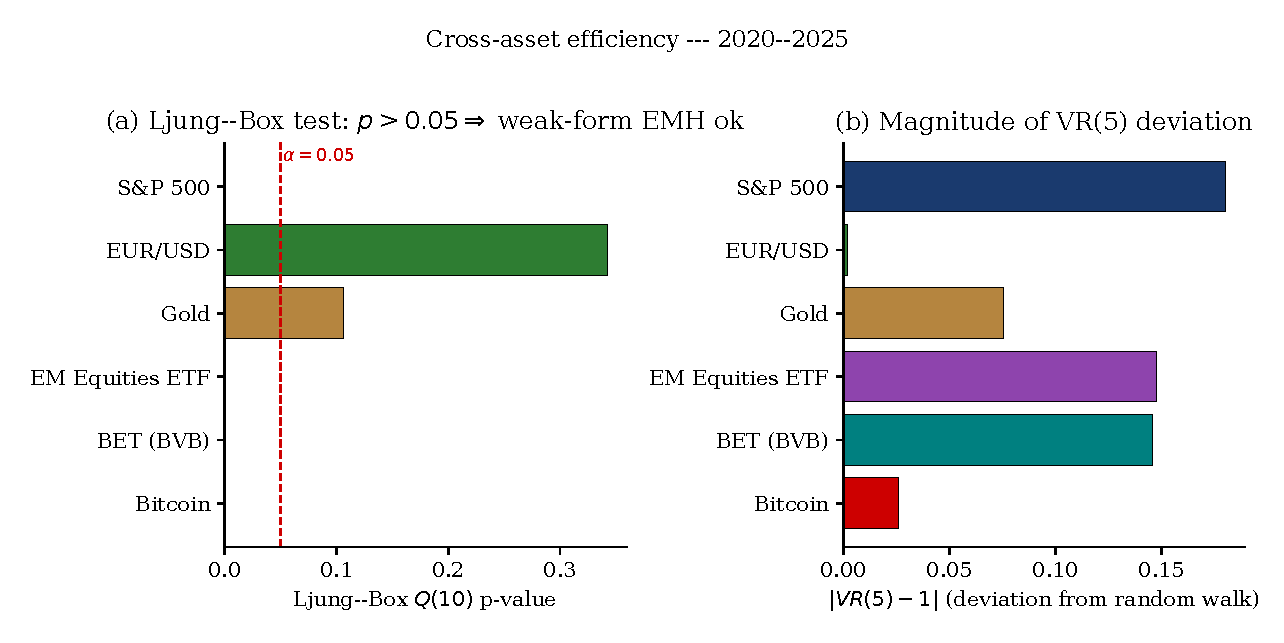
\includegraphics[width=\linewidth]{sfm_ch4_cross_asset.pdf}
\end{column}
\begin{column}{0.32\textwidth}
\footnotesize
\begin{itemize}\setlength{\itemsep}{0pt}
    \item \textbf{Citirea graficului}
    \begin{itemize}\setlength{\itemsep}{0pt}
        \item (a): bare la dreapta liniei roșii ($p > 0{,}05$) $\Rightarrow$ EMH slabă ok
        \item (b): bare scurte $\Rightarrow$ aproape de RW
    \end{itemize}
    \item \textbf{Clasament}
    \begin{itemize}\setlength{\itemsep}{0pt}
        \item Cel mai eficient: EUR/USD
        \item Aproape de RW: Aur
    \end{itemize}
    \item \textbf{Avertisment}
    \begin{itemize}\setlength{\itemsep}{0pt}
        \item COVID + post-COVID afectează $p$-value-urile pe indici de equity
    \end{itemize}
\end{itemize}
\end{column}
\end{columns}
\end{cminipage}
\vspace{0.05cm}
\quantlet{SFM\_ch4\_cross\_asset}{https://colab.research.google.com/github/QuantLet/Stat_fin_markets/blob/master/Ch_04/SFM_ch4_cross_asset/SFM_ch4_cross_asset.ipynb}
\end{frame}

\begin{frame}[shrink=15]{Studiu de caz 2: Bursa de Valori București (BVB) --- BET, TLV, FP}
\begin{cminipage}{0.95\textwidth}
\begin{columns}[T]
\begin{column}{0.6\textwidth}
\centering
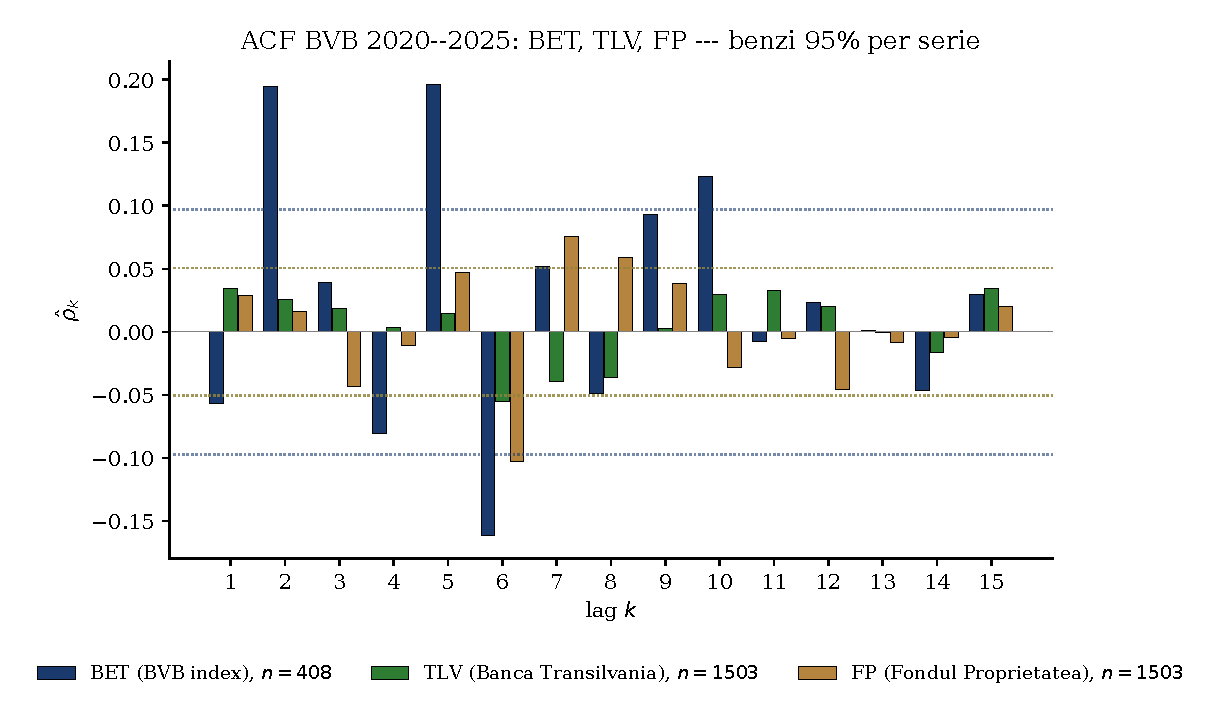
\includegraphics[width=\linewidth]{sfm_ch4_bvb_case.pdf}
\end{column}
\begin{column}{0.37\textwidth}
\footnotesize
\begin{itemize}\setlength{\itemsep}{0pt}
    \item \textbf{Date 2020--2025} (\textit{yfinance})
    \begin{itemize}\setlength{\itemsep}{0pt}
        \item BET (\texttt{\^{}BETI}): $n=408$, bandă $\pm 0{,}097$
        \item TLV.RO, FP.RO: $n=1503$, bandă $\pm 0{,}051$
    \end{itemize}
    \item \textbf{Pattern lag 1--2}
    \begin{itemize}\setlength{\itemsep}{0pt}
        \item BET: $\hat\rho_1=-0{,}06$ (în bandă), $\hat\rho_2=+0{,}20$ (afară)
        \item TLV, FP: $\hat\rho_1\approx 0{,}03$ (în bandă)
    \end{itemize}
    \item \textbf{Lag-uri afară din bandă}
    \begin{itemize}\setlength{\itemsep}{0pt}
        \item BET: $k\in\{2,5,6,10\}$ (multiple violări)
        \item FP: $k\in\{6,7,8\}$ (mean reversion lag 6)
    \end{itemize}
    \item \textbf{Cauze plauzibile}
    \begin{itemize}\setlength{\itemsep}{0pt}
        \item Thin trading, free-float mic
        \item Eșantion BET scurt $\Rightarrow$ bandă largă
    \end{itemize}
    \item \textbf{Test diagnostic:} eficiența crește pe date săptămânale?
\end{itemize}
\end{column}
\end{columns}
\end{cminipage}
\vspace{0.05cm}
\quantlet{SFM\_ch4\_bvb\_case}{https://colab.research.google.com/github/QuantLet/Stat_fin_markets/blob/master/Ch_04/SFM_ch4_bvb_case/SFM_ch4_bvb_case.ipynb}
\end{frame}

\begin{frame}[shrink=15]{Studiu de caz 3: Crypto vs piețe dezvoltate (BTC, ETH, S\&P)}
\begin{cminipage}{0.95\textwidth}
\begin{columns}[T]
\begin{column}{0.6\textwidth}
\centering
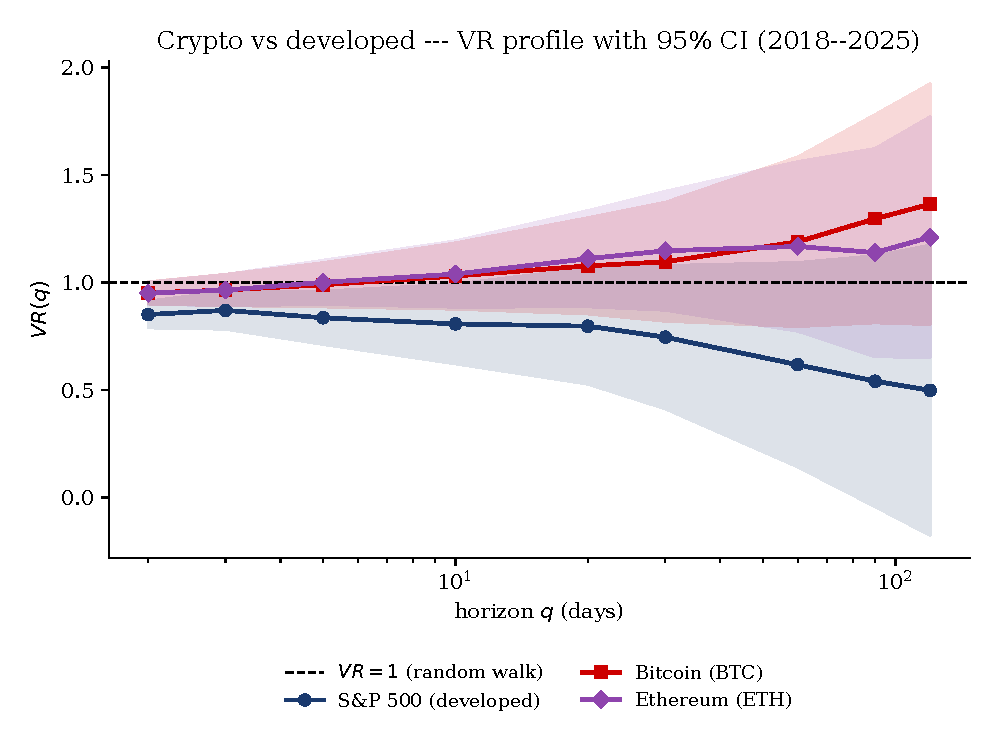
\includegraphics[width=\linewidth]{sfm_ch4_crypto_eff.pdf}
\end{column}
\begin{column}{0.37\textwidth}
\begin{itemize}\setlength{\itemsep}{0pt}
    \item \textbf{Date 2018--2025}
    \begin{itemize}\setlength{\itemsep}{0pt}
        \item BTC ($T = 2920$), ETH ($T = 2920$)
        \item S\&P 500 ($T = 2009$)
    \end{itemize}
    \item \textbf{Rezultate $\widehat{VR}(120)$}
    \begin{itemize}\setlength{\itemsep}{0pt}
        \item S\&P: $\approx 0{,}50$ (mean rev.\ post-COVID)
        \item BTC: $\approx 1{,}37$ (momentum)
        \item ETH: $\approx 1{,}21$ (similar BTC)
    \end{itemize}
    \item \textbf{Lecție AMH}
    \begin{itemize}\setlength{\itemsep}{0pt}
        \item Crypto = piață tânără, insuficient arbitrată
        \item Momentum statistic $\neq$ profit net
    \end{itemize}
\end{itemize}
\end{column}
\end{columns}
\end{cminipage}
\vspace{0.05cm}
\quantlet{SFM\_ch4\_crypto\_eff}{https://colab.research.google.com/github/QuantLet/Stat_fin_markets/blob/master/Ch_04/SFM_ch4_crypto_eff/SFM_ch4_crypto_eff.ipynb}
\end{frame}

\begin{frame}[shrink=15]{Studiu de caz 4: FX major --- piețele textbook eficiente}
\begin{cminipage}{0.95\textwidth}
\begin{columns}[T]
\begin{column}{0.6\textwidth}
\centering
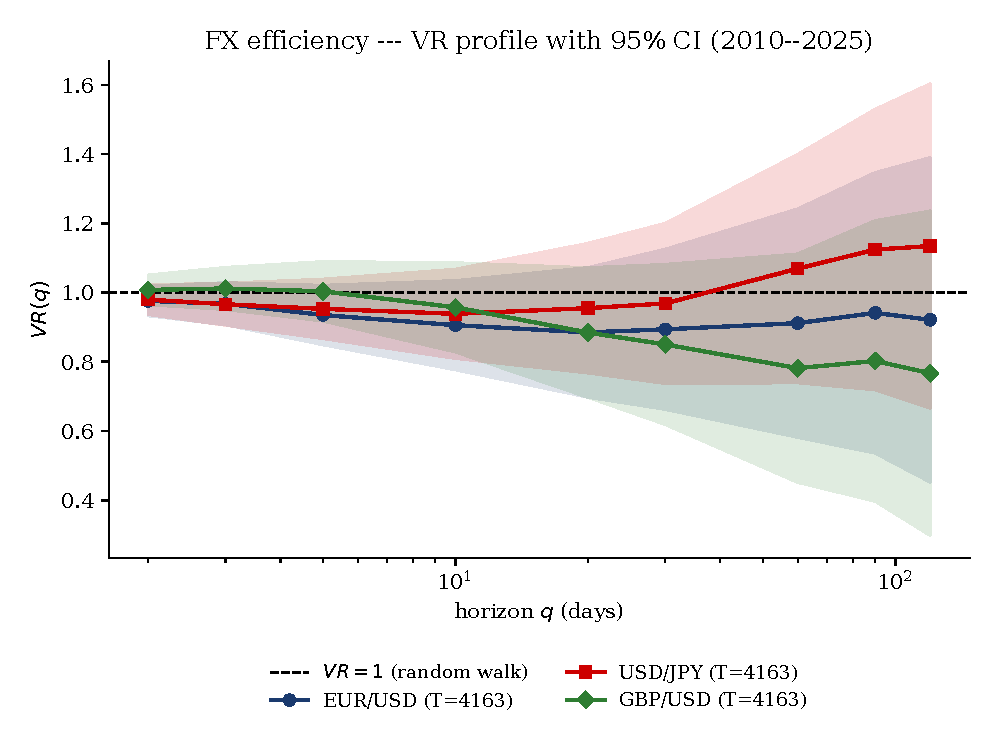
\includegraphics[width=\linewidth]{sfm_ch4_fx_efficiency.pdf}
\end{column}
\begin{column}{0.37\textwidth}
\begin{itemize}\setlength{\itemsep}{0pt}
    \item EUR/USD, USD/JPY, GBP/USD --- 2010--2025 zilnic, $T = 4163$
    \item \textbf{Observație:} $\widehat{VR}(q)$ aproape de $1$ pe toate orizonturile
    \item IC 95\% cuprinde valoarea $1$ pe majoritatea $q$-urilor
    \item De ce sunt FX atât de eficiente?
    \begin{itemize}\setlength{\itemsep}{0pt}
        \item Lichiditate masivă ($> \$7$ trilioane/zi)
        \item Tranzacționare 24/5
        \item Mulți participanți informați
        \item Costuri foarte mici (sub 1bp)
    \end{itemize}
    \item \textbf{Comparație:} FX major $>$ S\&P $>$ crypto $>$ EM
\end{itemize}
\end{column}
\end{columns}
\end{cminipage}
\vspace{0.05cm}
\quantlet{SFM\_ch4\_fx\_efficiency}{https://colab.research.google.com/github/QuantLet/Stat_fin_markets/blob/master/Ch_04/SFM_ch4_fx_efficiency/SFM_ch4_fx_efficiency.ipynb}
\end{frame}

\begin{frame}[shrink=15]{Studiu de caz 5: Eficiența S\&P 500 pe sub-perioade}
\begin{cminipage}{0.95\textwidth}
\begin{columns}[T]
\begin{column}{0.7\textwidth}
\centering
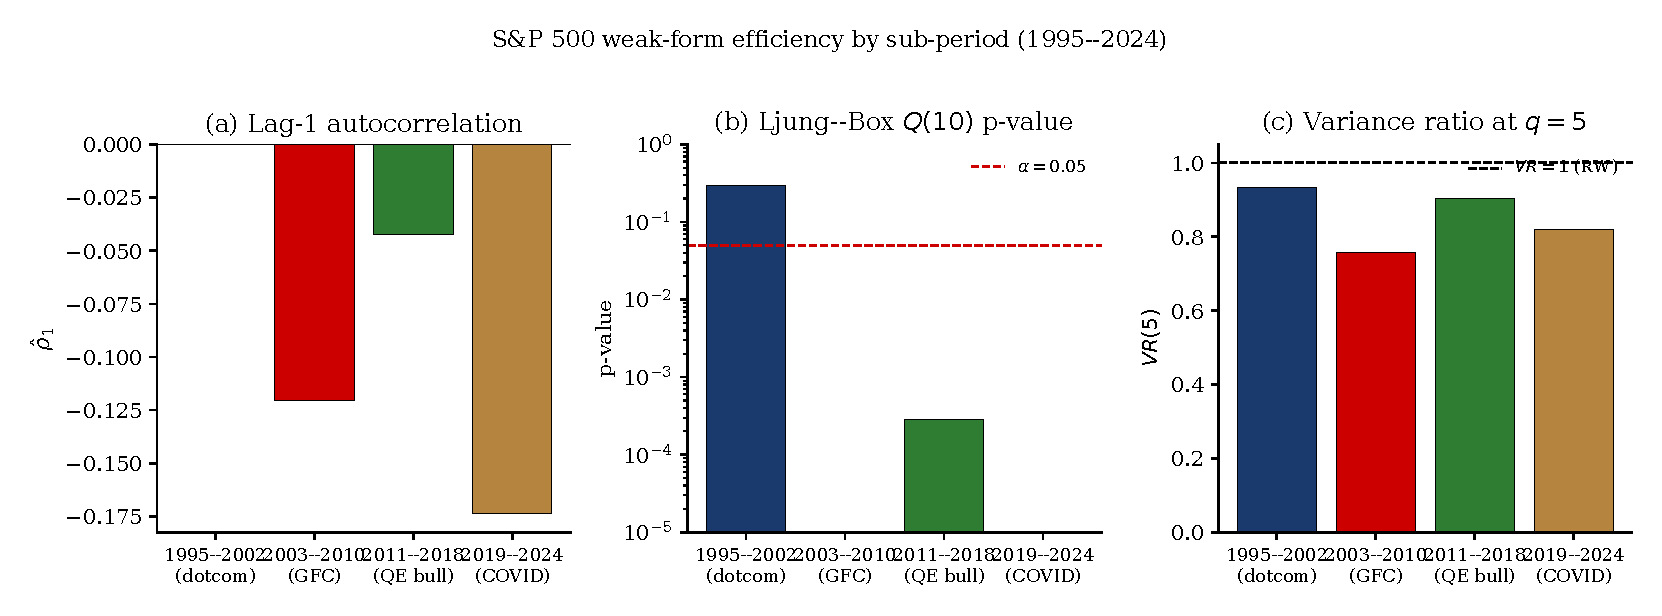
\includegraphics[width=\linewidth]{sfm_ch4_subperiod_efficiency.pdf}
\end{column}
\begin{column}{0.28\textwidth}
\footnotesize
\begin{itemize}\setlength{\itemsep}{0pt}
    \item \textbf{4 sub-perioade}
    \begin{itemize}\setlength{\itemsep}{0pt}
        \item Dotcom 1995--2002
        \item GFC (Global Financial Crisis) 2003--2010
        \item QE (Quantitative Easing) bull 2011--2018
        \item COVID 2019--2024
    \end{itemize}
    \item \textbf{Ineficiență}
    \begin{itemize}\setlength{\itemsep}{0pt}
        \item GFC: $\hat\rho_1 \approx -0{,}12$
        \item COVID: $\hat\rho_1 \approx -0{,}17$
    \end{itemize}
    \item \textbf{Eficiență}
    \begin{itemize}\setlength{\itemsep}{0pt}
        \item QE bull: $\hat\rho_1 \approx -0{,}04$
    \end{itemize}
    \item \textbf{Concluzie AMH}
    \begin{itemize}\setlength{\itemsep}{0pt}
        \item Eficiența depinde de regim
    \end{itemize}
\end{itemize}
\end{column}
\end{columns}
\end{cminipage}
\vspace{0.05cm}
\quantlet{SFM\_ch4\_subperiod\_efficiency}{https://colab.research.google.com/github/QuantLet/Stat_fin_markets/blob/master/Ch_04/SFM_ch4_subperiod_efficiency/SFM_ch4_subperiod_efficiency.ipynb}
\end{frame}

\begin{frame}[shrink=15]{Studiu de caz 6: Bootstrap vs IC asimptotic pentru VR (BTC)}
\begin{cminipage}{0.95\textwidth}
\begin{columns}[T]
\begin{column}{0.6\textwidth}
\centering
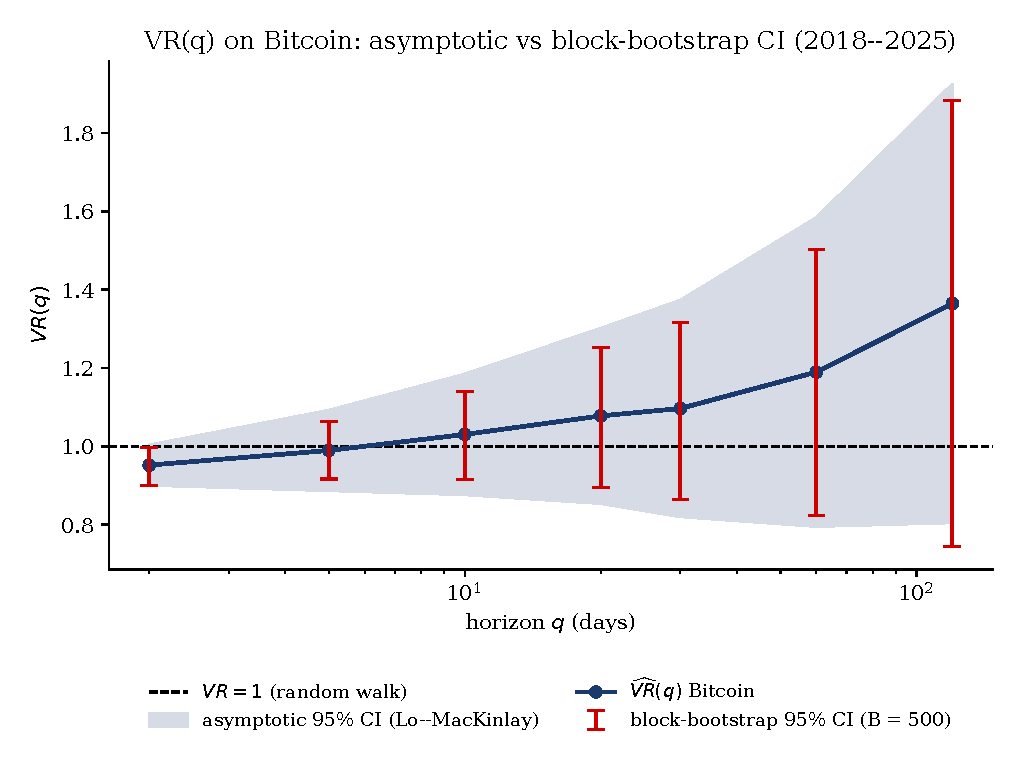
\includegraphics[width=\linewidth]{sfm_ch4_vr_bootstrap_ci.pdf}
\end{column}
\begin{column}{0.37\textwidth}
\begin{itemize}\setlength{\itemsep}{0pt}
    \item \textbf{Întrebare:} formula $SE = \sqrt{2(q-1)/T}$ presupune homoscedasticitate. Cât e de bună pe BTC?
    \item \textbf{Comparație}
    \begin{itemize}\setlength{\itemsep}{0pt}
        \item IC asimptotic (bandă albastră)
        \item IC bootstrap pe blocuri (bare roșii), $B = 500$
    \end{itemize}
    \item \textbf{Observație:} bootstrap ușor mai îngust pe BTC
    \item \textbf{Lecție generală:} IC bootstrap este mai robust la cozi grele, clustering volatilitate; recomandat pentru active cu $\alpha < 2$
\end{itemize}
\end{column}
\end{columns}
\end{cminipage}
\vspace{0.05cm}
\quantlet{SFM\_ch4\_vr\_bootstrap\_ci}{https://colab.research.google.com/github/QuantLet/Stat_fin_markets/blob/master/Ch_04/SFM_ch4_vr_bootstrap_ci/SFM_ch4_vr_bootstrap_ci.ipynb}
\end{frame}

%=============================================================================
% PARTEA X: AI CHECKS + DISCUȚII
%=============================================================================
\section{Partea X: AI checks și discuții}

\begin{frame}[shrink=15]{Exercițiu AI 1: Prompt engineering pentru analiza EMH}
\begin{cminipage}{0.95\textwidth}
\vspace{-3mm}
\begin{block}{\footnotesize Prompt de testat (cereți LLM, Large Language Model)}
\footnotesize
\begin{itemize}\setlength{\itemsep}{0pt}
    \item \textbf{Date:} descarcă randamente zilnice S\&P 500 (ultimii 10 ani)
    \item \textbf{Teste forma slabă:}
    \begin{itemize}\setlength{\itemsep}{0pt}
        \item Autocorelație la lag 1--20 + Ljung--Box
        \item Variance ratio $VR(q)$ pentru $q \in \{2, 5, 10, 20\}$ cu IC 95\% (Lo--MacKinlay)
    \end{itemize}
    \item \textbf{Output:} raportează care orizonturi $q$ resping RW, apoi concluzionează
\end{itemize}
\end{block}
\vspace{-2mm}
\begin{block}{\footnotesize Verificați}
\footnotesize
\begin{itemize}\setlength{\itemsep}{0pt}
    \item \textbf{Date:} LLM folosește \texttt{yfinance} corect (ticker \texttt{\^{}GSPC})?
    \item \textbf{Formule:}
    \begin{itemize}\setlength{\itemsep}{0pt}
        \item Autocorelație corectă ($\hat\gamma_k / \hat\gamma_0$)?
        \item Ljung--Box cu corecția $(n+2)$ (vs Box--Pierce)?
        \item VR: corecție heteroscedasticitate?
        \item $Z$ pentru VR cu $\sqrt{2(q-1)/T}$?
    \end{itemize}
    \item \textbf{Concluzia:} nuanțată (nu da/nu categoric)?
\end{itemize}
\end{block}
\vspace{-2mm}
\begin{alertblock}{Atenție}
\footnotesize
\begin{itemize}\setlength{\itemsep}{0pt}
    \item LLM-ul poate genera concluzii prea categorice
    \item Eficiența este chestiune de \emph{grad}, nu de da/nu
\end{itemize}
\end{alertblock}
\end{cminipage}
\end{frame}

\begin{frame}[shrink=15]{Exercițiu AI 2: Verificarea codului LLM --- Event Study}
\begin{cminipage}{0.95\textwidth}
\begin{columns}[T]
\begin{column}{0.48\textwidth}
\begin{block}{\footnotesize Prompt de testat}
\footnotesize
\begin{itemize}\setlength{\itemsep}{0pt}
    \item \textbf{Date}
    \begin{itemize}\setlength{\itemsep}{0pt}
        \item AAPL + S\&P 500 zilnic
    \end{itemize}
    \item \textbf{Event study AAPL Q4 2024}
    \begin{itemize}\setlength{\itemsep}{0pt}
        \item Estimare $[-250, -11]$
        \item Eveniment $[-5, +5]$
        \item AR, CAR, IC 95\%
    \end{itemize}
    \item \textbf{Vizualizare}
    \begin{itemize}\setlength{\itemsep}{0pt}
        \item CAR cu bandă umbrită
    \end{itemize}
\end{itemize}
\end{block}
\end{column}
\begin{column}{0.48\textwidth}
\begin{block}{\footnotesize Verificați}
\footnotesize
\begin{itemize}\setlength{\itemsep}{0pt}
    \item \textbf{Ferestre}
    \begin{itemize}\setlength{\itemsep}{0pt}
        \item Estimare vs eveniment fără suprapunere?
    \end{itemize}
    \item \textbf{Modelul de piață}
    \begin{itemize}\setlength{\itemsep}{0pt}
        \item OLS (Ordinary Least Squares) pe $R_i = \alpha + \beta R_m + \varepsilon$?
        \item $AR = R_i - \hat{R}_i$?
    \end{itemize}
    \item \textbf{IC pentru CAR}
    \begin{itemize}\setlength{\itemsep}{0pt}
        \item $\hat\sigma_\varepsilon$ din estimare?
        \item Cu $\sqrt{|t-t_0|}$?
    \end{itemize}
\end{itemize}
\end{block}
\end{column}
\end{columns}
\vspace{0.1cm}
\begin{alertblock}{Atenție}
\footnotesize
\begin{itemize}\setlength{\itemsep}{0pt}
    \item LLM-urile confundă des fereastra de estimare cu cea a evenimentului
    \item Verificați că $\hat\alpha, \hat\beta$ sunt estimați \textbf{exclusiv} pe date pre-event
\end{itemize}
\end{alertblock}
\end{cminipage}
\end{frame}

\begin{frame}[shrink=15]{Discuție 1: EMH în practică}
\begin{cminipage}{0.95\textwidth}
\begin{itemize}\setlength{\itemsep}{0pt}
    \item \textbf{Scenariu:} Un fond quantitativ dezvoltă o strategie de tranzacționare bazată pe mean reversion, exploatând faptul că $VR(5) \approx 0{,}85$ pe un indice bursier. Strategia funcționează 2 ani, apoi devine neprofitabilă.
    \item \textbf{Întrebări:}
\end{itemize}
\begin{enumerate}\setlength{\itemsep}{0pt}
    \item De ce strategia a funcționat inițial? (Ineficiență temporară, lichiditate redusă)
    \item De ce a încetat să funcționeze? (Alți participanți au descoperit aceeași anomalie)
    \item Cum se încadrează aceasta în \textbf{AMH} (Lo, 2004)?
    \item Ce rol joacă \textbf{costurile de tranzacție} în definirea eficienței?
\end{enumerate}

\vspace{0.2cm}
\begin{block}{Recomandare}
\small
\begin{itemize}\setlength{\itemsep}{0pt}
    \item Eficiența nu este o proprietate binară
    \item O piață poate fi ,,eficientă net de costuri'' chiar dacă există predictibilitate statistică
    \item Profitul trebuie să depășească spread-ul, comisioanele și slippage-ul
\end{itemize}
\end{block}
\end{cminipage}
\end{frame}

\begin{frame}[shrink=15]{Discuție 2: Limitările testelor de eficiență}
\begin{cminipage}{0.95\textwidth}
\begin{itemize}\setlength{\itemsep}{0pt}
    \item \textbf{Scenariu:} Aplicați testul Ljung--Box pe randamentele zilnice BET (indicele BVB) și obțineți $Q(10) = 25{,}3$, $p = 0{,}005$. Concluzia naivă: ,,BVB este ineficientă.''
    \item \textbf{Întrebări:}
\end{itemize}
\begin{enumerate}\setlength{\itemsep}{0pt}
    \item Ce presupune Ljung--Box despre distribuția randamentelor? (Momente finite, staționaritate)
    \item Dacă randamentele au cozi grele ($\alpha < 2$), testul este \textbf{valid}?
    \item Autocorelația poate fi cauzată de \textbf{thin trading} (tranzacționare rară)?
    \item Care este diferența între \textbf{semnificație statistică} și \textbf{semnificație economică}?
\end{enumerate}

\vspace{0.2cm}
\begin{itemize}\setlength{\itemsep}{0pt}
    \item \textbf{Indiciu:} Pe BVB, autocorelația este adesea cauzată de non-sincronizarea tranzacțiilor, nu de ineficiență reală. Testați cu date \textbf{săptămânale} pentru a elimina efectul thin trading.
\end{itemize}
\end{cminipage}
\end{frame}

%=============================================================================
% PARTEA XI: STUDIU DE CAZ S&P 500 + TEMĂ BVB
%=============================================================================
\section{Partea XI: Studiu de caz S\&P 500 \& temă BVB}

% ---------- Studiu cap-coadă pe S&P 500 (date reale via yfinance) ----------
\begin{frame}[shrink=12]{Studiu cap-coadă: S\&P 500 2015--2024 (\^{}GSPC, $n=2514$)}
\begin{cminipage}{0.97\textwidth}
\begin{columns}[T]
\begin{column}{0.66\textwidth}
\centering
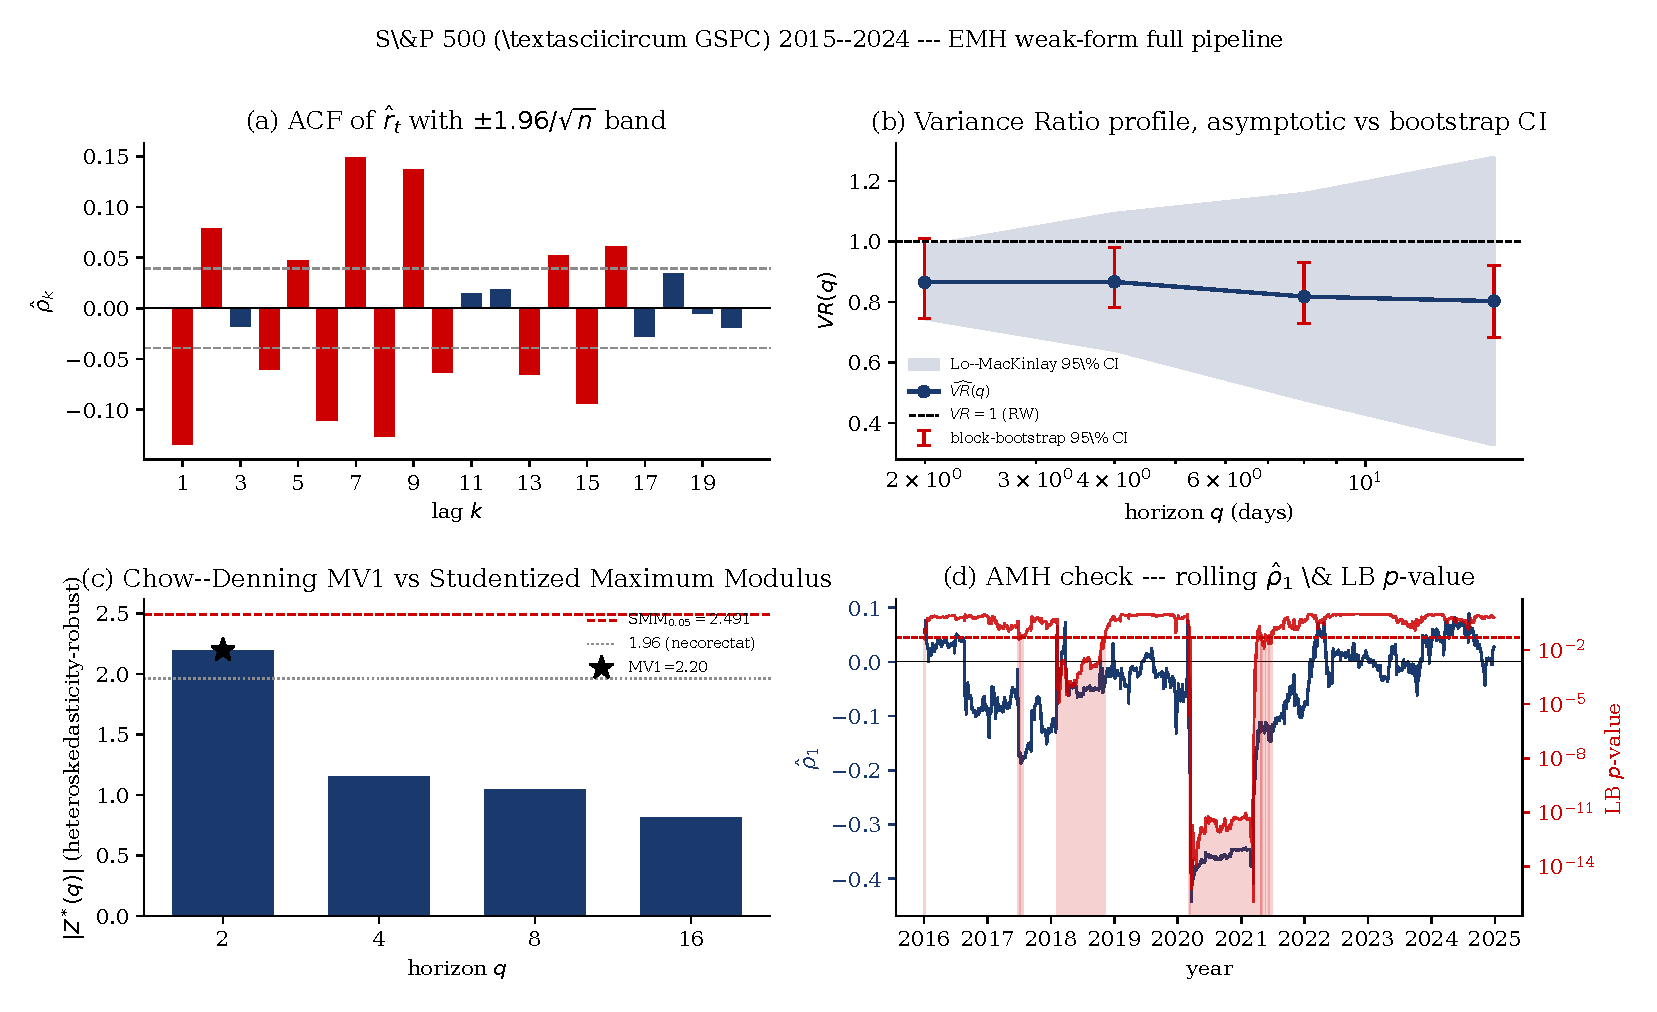
\includegraphics[width=\linewidth]{sfm_ch4_full_pipeline.pdf}
\end{column}
\begin{column}{0.32\textwidth}
\footnotesize
\begin{itemize}\setlength{\itemsep}{0pt}
    \item \textbf{Date}: yfinance, log-randamente
    \begin{itemize}\setlength{\itemsep}{0pt}
        \item $n = 2514$, $\bar r = 0{,}042\%$/zi
        \item $\hat\sigma = 1{,}13\%$/zi ($17{,}9\%$/an)
    \end{itemize}
    \item \textbf{Pipeline complet}
    \begin{itemize}\setlength{\itemsep}{0pt}
        \item (a) ACF $\hat\rho_k$ cu bandă $\pm 1{,}96/\sqrt{n}$
        \item (b) VR$(q)$ + IC asimptotic Lo--MacKinlay + IC block-bootstrap
        \item (c) Chow--Denning MV1 vs SMM
        \item (d) AMH: $\hat\rho_1$ și LB $p$-value rolling 1 an
    \end{itemize}
    \item \textbf{Verdict global}
    \begin{itemize}\setlength{\itemsep}{0pt}
        \item ACF/Ljung--Box: respinge RW (lag-uri multiple)
        \item VR/Chow--Denning: $\mathrm{MV1}=2{,}20<2{,}49$ $\Rightarrow$ \textbf{nu} respinge RW (IC conțin 1)
        \item Economic: deviații mici, greu de exploatat net de costuri
    \end{itemize}
\end{itemize}
\end{column}
\end{columns}
\end{cminipage}
\vspace{0.05cm}
\quantlet{SFM\_ch4\_full\_pipeline}{https://colab.research.google.com/github/QuantLet/Stat_fin_markets/blob/master/Ch_04/SFM_ch4_full_pipeline/SFM_ch4_full_pipeline.ipynb}
\end{frame}

\begin{frame}[shrink=12]{Pipeline detaliat 1/3 --- ACF, Ljung--Box, Runs}
\begin{cminipage}{0.95\textwidth}
\begin{block}{Teste liniare pe lag-uri scurte (S\&P 500, $n=2514$)}
\renewcommand{\arraystretch}{1.05}
\footnotesize
\begin{tabular}{lllll}
\toprule
\textbf{Test} & \textbf{Statistică} & \textbf{Critic / band} & \textbf{$p$-value} & \textbf{Decizie} \\
\midrule
$\hat\rho_1$            & $-0{,}1348$        & $\pm 0{,}0391$       & $\approx 0$ & Respinge \\
$\hat\rho_2$            & $+0{,}0786$        & $\pm 0{,}0391$       & $< 0{,}001$ & Respinge \\
max $|\hat\rho_k|$ ($k=1..20$) & $+0{,}1490$ (lag 7) & $\pm 0{,}0391$ & $< 0{,}001$ & Respinge \\
Ljung--Box $Q(10)$      & $262{,}0$          & $\chi^2_{0{,}05}(10)=18{,}3$ & $< 10^{-50}$ & Respinge tare \\
Ljung--Box $Q(20)$      & $318{,}7$          & $\chi^2_{0{,}05}(20)=31{,}4$ & $< 10^{-55}$ & Respinge tare \\
Runs test (semne)       & $Z = +2{,}43$      & $|Z|>1{,}96$         & $0{,}015$   & Respinge \\
\bottomrule
\end{tabular}
\end{block}
\begin{itemize}\setlength{\itemsep}{0pt}
    \item \textbf{Citire}: $\hat\rho_1 = -0{,}13$ \emph{semnificativ negativ} $\Rightarrow$ ușor mean reversion la 1 zi
    \item \textbf{Lag-uri semnificative} (banda $\pm 0{,}039$): $k \in \{1,2,4,5,6,7,8,9,10,13,14,15,16\}$
    \item \textbf{LB respinge masiv}: $Q(10)=262$ vs critic $18{,}3$ --- dependență liniară prezentă
    \item \textbf{Runs}: $R = 1311$ vs $\mathbb{E}[R] = 1250$, $Z = +2{,}43$ $\Rightarrow$ alternare ușor excesivă
    \item \alert{Atenție}: COVID 2020 contribuie major la $\hat\rho_1$ (efect crash + recovery)
\end{itemize}
\end{cminipage}
\end{frame}

\begin{frame}[shrink=12]{Pipeline detaliat 2/3 --- Variance Ratio cu dublu IC}
\begin{cminipage}{0.95\textwidth}
\begin{block}{$\widehat{VR}(q)$ cu IC 95\% Lo--MacKinlay (asimptotic) și block-bootstrap (B=500)}
\renewcommand{\arraystretch}{1.05}
\footnotesize
\begin{tabular}{rrrrcc}
\toprule
$q$ & $\widehat{VR}(q)$ & SE & $|Z^*|$ (LM) & IC LM 95\% & IC bootstrap 95\% \\
\midrule
$2$  & $0{,}8648$ & $0{,}0615$ & $\mathbf{2{,}20}$ & $[0{,}744;\, 0{,}985]$ & $[0{,}745;\, 1{,}011]$ \\
$4$  & $0{,}8663$ & $0{,}1155$ & $1{,}16$           & $[0{,}640;\, 1{,}093]$ & $[0{,}781;\, 0{,}979]$ \\
$8$  & $0{,}8178$ & $0{,}1740$ & $1{,}05$           & $[0{,}477;\, 1{,}159]$ & $[0{,}728;\, 0{,}929]$ \\
$16$ & $0{,}8028$ & $0{,}2425$ & $0{,}81$           & $[0{,}328;\, 1{,}278]$ & $[0{,}683;\, 0{,}922]$ \\
\bottomrule
\end{tabular}
\end{block}
\begin{itemize}\setlength{\itemsep}{0pt}
    \item \textbf{Tipar}: $\widehat{VR}(q) \in [0{,}80; 0{,}87]$ pentru toate $q$ $\Rightarrow$ ușor \emph{mean reversion}
    \item \textbf{Lo--MacKinlay}: respinge RW \emph{doar} la $q=2$ ($|Z^*|=2{,}20$); SE crește rapid cu $q$
    \item \textbf{Block-bootstrap}: \emph{exclude} valoarea $1$ pentru $q \in \{4, 8, 16\}$ --- mult mai puternic
    \item \alert{Lecție}: bootstrap-ul, robust la cozi grele și clustering volatilitate, depistează ineficiența ascunsă de IC asimptotic la $q$ mari
\end{itemize}
\end{cminipage}
\end{frame}

\begin{frame}[shrink=12]{Pipeline detaliat 3/3 --- Chow--Denning MV1 + AMH rolling}
\begin{cminipage}{0.95\textwidth}
\begin{columns}[T]
\begin{column}{0.48\textwidth}
\begin{block}{Chow--Denning MV1 (test simultan)}
\footnotesize
\begin{itemize}\setlength{\itemsep}{0pt}
    \item $\mathrm{MV1} = \max_{q \in \{2,4,8,16\}} |Z^*(q)| = 2{,}199$ (la $q=2$)
    \item Critic SMM$_{0{,}05}$ ($m=4$, $\nu=\infty$) $= 2{,}491$ (Stoline--Ury, 1979)
    \item $\mathrm{MV1} = 2{,}20 < 2{,}491 \Rightarrow$ \textbf{nu respinge} EMH slabă (ajustat)
    \item Pragul necorectat $1{,}96$ ar fi respins fals la $q=2$
\end{itemize}
\end{block}
\begin{block}{Reconciliere asimptotic vs bootstrap}
\footnotesize
\begin{itemize}\setlength{\itemsep}{0pt}
    \item Asimptotic (LM, MV1): \emph{nu respinge} la nivel comun
    \item Bootstrap: \emph{respinge} la $q \in \{4, 8, 16\}$
    \item Diferență: SE asimptotic prea conservator pe cozi grele
\end{itemize}
\end{block}
\end{column}
\begin{column}{0.48\textwidth}
\begin{block}{Adaptive Markets Hypothesis --- rolling 1 an}
\footnotesize
\begin{itemize}\setlength{\itemsep}{0pt}
    \item Fereastră: 252 zile, alunecată zilnic
    \item $\hat\rho_1$ rolling: interval $[-0{,}442;\, +0{,}088]$
    \item $\hat\rho_1$ mediu: $-0{,}065$ (ușor negativ)
    \item Ferestre cu LB $Q(5)$ $p<0{,}05$: \textbf{22{,}3\%}
    \item Vârfuri de ineficiență: 2018 (Volpocalypse), 2020 (COVID), 2022 (Fed)
    \item Perioade calme: 2017, 2024
\end{itemize}
\end{block}
\begin{alertblock}{Verdict cantitativ}
\footnotesize
S\&P 500 (2015--2024) este \emph{predominant} eficient slabă, dar cu ferestre de ineficiență tranzitorii corelate cu stres de piață (consistent cu Lo, 2004).
\end{alertblock}
\end{column}
\end{columns}
\end{cminipage}
\end{frame}

\begin{frame}[shrink=15]{S\&P 500: Eficiența variază în timp (AMH)}
\begin{cminipage}{0.95\textwidth}
\begin{columns}[T]
\begin{column}{0.48\textwidth}
\begin{block}{Perioade de ineficiență}
\begin{itemize}\setlength{\itemsep}{0pt}
    \item \textbf{2008--2009:} Criza financiară
    \begin{itemize}\setlength{\itemsep}{0pt}
        \item $VR(5) \approx 0{,}82$; $\hat\rho_1 \approx -0{,}11$
        \item Ljung--Box $Q(10)$ semnificativ ($p < 0{,}01$)
        \item Panică $\Rightarrow$ mean reversion puternic
    \end{itemize}
    \item \textbf{2020 (martie):} COVID-19
    \begin{itemize}\setlength{\itemsep}{0pt}
        \item Autocorelație negativă: $\hat\rho_1 \approx -0{,}13$
        \item Suprareacție urmată de recovery rapid
    \end{itemize}
\end{itemize}
\end{block}
\end{column}
\begin{column}{0.48\textwidth}
\begin{block}{Perioade de eficiență}
\begin{itemize}\setlength{\itemsep}{0pt}
    \item \textbf{2013--2017:} Bull market stabil
    \begin{itemize}\setlength{\itemsep}{0pt}
        \item $VR(5) \approx 0{,}99$, $\hat\rho_1 \approx 0$
        \item Ljung--Box nesemnificativ
        \item Piață ,,calmă și eficientă''
    \end{itemize}
    \item \textbf{2023--2024:} Post-criză
    \begin{itemize}\setlength{\itemsep}{0pt}
        \item $\hat\rho_1$ apropiat de zero
        \item Lichiditate crescută
    \end{itemize}
\end{itemize}
\end{block}
\end{column}
\end{columns}

\vspace{0.2cm}
\begin{alertblock}{Adaptive Markets Hypothesis (Lo, 2004)}
\small
\begin{itemize}\setlength{\itemsep}{0pt}
    \item Eficiența nu este fixă, ci un \textbf{proces dinamic}
    \item Piețele devin mai eficiente în perioade calme
    \item Și mai puțin eficiente în crize
\end{itemize}
\end{alertblock}
\end{cminipage}
\end{frame}

\begin{frame}[shrink=15]{Temă: Eficiența pieței pe BVB}
\begin{cminipage}{0.95\textwidth}
\begin{block}{Cerințe}
\begin{enumerate}\setlength{\itemsep}{0pt}
    \item Alegeți o acțiune listată la BVB (ex: TLV, SNP, BRD, FP)
    \item Descărcați datele zilnice din ultimii 5 ani (\texttt{yfinance}, ticker ex: \texttt{TLV.RO})
    \item Calculați autocorelația la lag 1--10 și testul Ljung--Box
    \item Calculați variance ratio $VR(q)$ pentru $q \in \{2, 4, 8, 16\}$ cu IC 95\% și MV1 Chow--Denning
    \item Aplicați și runs test pe semnele randamentelor
    \item Comparați cu S\&P 500: este BVB mai ,,eficientă'' sau mai ,,ineficientă''?
    \item Interpretați diferențele (lichiditate, nr.\ participanți, informație)
\end{enumerate}
\end{block}

\vspace{0.1cm}
\begin{exampleblock}{Indicii}
\begin{itemize}\setlength{\itemsep}{0pt}
    \item Piețele emergente sunt de obicei \textit{mai puțin} eficiente (lichiditate redusă)
    \item BVB poate avea autocorelație mai mare datorită tranzacționării rare (thin trading)
    \item Folosiți quantlets disponibile (Colab) ca punct de plecare
    \item \textbf{Bonus:} Aplicați testele pe ferestre rolling de 1 an pentru a identifica perioade de (in)eficiență
\end{itemize}
\end{exampleblock}
\end{cminipage}
\end{frame}

\begin{frame}[shrink=15]{Hartă decizională --- cum testăm EMH în practică}
\begin{cminipage}{0.95\textwidth}
\begin{center}
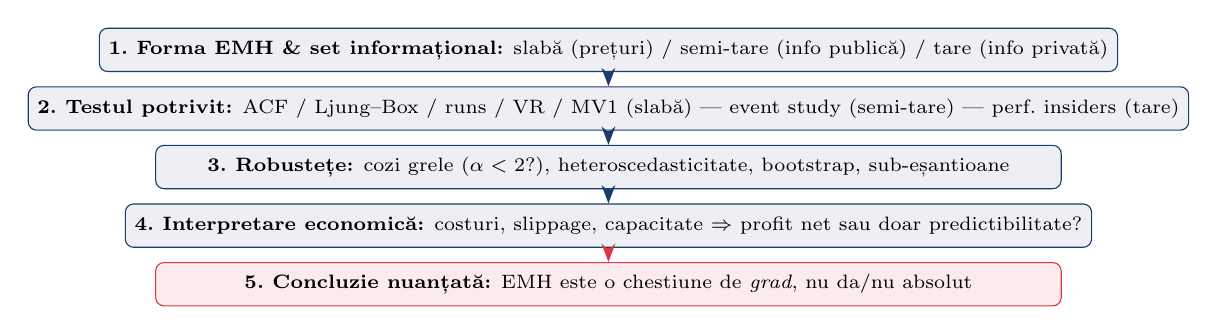
\begin{tikzpicture}[
    node distance=0.18cm,
    every node/.style={font=\scriptsize, align=center},
    pasul/.style={draw=MainBlue, fill=MainBlue!8, rounded corners=3pt,
                 minimum width=11.5cm, minimum height=0.55cm}
]
\node[pasul] (s1) {\textbf{1.\ Forma EMH \& set informațional:} slabă (prețuri) / semi-tare (info publică) / tare (info privată)};
\node[pasul, below=of s1] (s2) {\textbf{2.\ Testul potrivit:} ACF / Ljung--Box / runs / VR / MV1 (slabă) --- event study (semi-tare) --- perf.\ insiders (tare)};
\node[pasul, below=of s2] (s3) {\textbf{3.\ Robustețe:} cozi grele ($\alpha < 2$?), heteroscedasticitate, bootstrap, sub-eșantioane};
\node[pasul, below=of s3] (s4) {\textbf{4.\ Interpretare economică:} costuri, slippage, capacitate $\Rightarrow$ profit net sau doar predictibilitate?};
\node[pasul, fill=Crimson!10, draw=Crimson, below=of s4] (s5) {\textbf{5.\ Concluzie nuanțată:} EMH este o chestiune de \emph{grad}, nu da/nu absolut};
\draw[-{Stealth}, MainBlue, thick] (s1) -- (s2);
\draw[-{Stealth}, MainBlue, thick] (s2) -- (s3);
\draw[-{Stealth}, MainBlue, thick] (s3) -- (s4);
\draw[-{Stealth}, Crimson, thick] (s4) -- (s5);
\end{tikzpicture}
\end{center}

\vspace{0.1cm}
\begin{alertblock}{Mesaj final}
\footnotesize
\begin{itemize}\setlength{\itemsep}{0pt}
    \item \textbf{Eficiența nu este binară}
    \begin{itemize}\setlength{\itemsep}{0pt}
        \item Cât de eficientă, pe ce orizont, sub ce costuri, pentru cine?
    \end{itemize}
\end{itemize}
\end{alertblock}
\end{cminipage}
\end{frame}

%=============================================================================
% PARTEA XII: QUIZ + CONCLUZII
%=============================================================================
\section{Partea XII: Quiz și concluzii}

\begin{frame}[shrink=15]{Adevărat sau Fals? (1/3)}
\begin{cminipage}{0.95\textwidth}
\footnotesize
\begin{columns}[T]
\begin{column}{0.48\textwidth}
\begin{enumerate}\setlength{\itemsep}{1pt}
    \item \textit{,,Dacă piața este eficientă, prețurile se mișcă aleatoriu.''}
    \item[] \textcolor{Forest}{\textbf{Adevărat.}} Randamentele sunt impredictibile $\Rightarrow$ random walk (aproximativ).

    \item \textit{,,EMH implică prețuri corecte în orice moment.''}
    \item[] \textcolor{Crimson}{\textbf{Fals.}} EMH implică doar că \textit{abaterile} nu sunt predictibile. Bule pot exista.

    \item \textit{,,$VR(q) = 1$ demonstrează eficiența pieței.''}
    \item[] \textcolor{Crimson}{\textbf{Fals.}} $VR=1$ este condiție \textit{necesară} dar nu \textit{suficientă}. Testează doar forma slabă.

    \item \textit{,,IC 95\% pentru $VR(q)$ care exclude valoarea $1$ respinge random walk.''}
    \item[] \textcolor{Forest}{\textbf{Adevărat.}} Echivalent cu testul $|Z(q)| > 1{,}96$.
\end{enumerate}
\end{column}
\begin{column}{0.48\textwidth}
\begin{enumerate}\setlength{\itemsep}{1pt}
    \setcounter{enumi}{4}
    \item \textit{,,Insider trading demonstrează că piața nu este eficientă forma tare.''}
    \item[] \textcolor{Forest}{\textbf{Adevărat.}} Dacă insiderii obțin profit sistematic, informația privată nu este reflectată.

    \item \textit{,,Autocorelația zero a randamentelor implică independență.''}
    \item[] \textcolor{Crimson}{\textbf{Fals.}} Autocorelația măsoară doar dependența \textit{liniară}. $r_t^2$ poate fi autocorelat.

    \item \textit{,,AMH contrazice EMH.''}
    \item[] \textcolor{Crimson}{\textbf{Fals.}} AMH este o \textit{generalizare}. EMH este un caz special al AMH.
\end{enumerate}
\end{column}
\end{columns}
\end{cminipage}
\end{frame}

\begin{frame}[shrink=15]{Adevărat sau Fals? (2/3)}
\begin{cminipage}{0.95\textwidth}
\begin{columns}[T]
\begin{column}{0.48\textwidth}
\begin{itemize}\setlength{\itemsep}{1pt}
    \item ,,EMH implică randamente zero.''
    \begin{itemize}\setlength{\itemsep}{0pt}
        \item[] \textcolor{Crimson}{\textbf{Fals.}} EMH cere doar ca \emph{randamentele neașteptate} să fie zero în medie. Investitorii câștigă prima de risc.
    \end{itemize}
    \item ,,EMH $\Leftrightarrow$ random walk.''
    \begin{itemize}\setlength{\itemsep}{0pt}
        \item[] \textcolor{Crimson}{\textbf{Fals.}} EMH implică martingal pt.\ prețuri ajustate la risc, nu incremente iid. GARCH compatibil.
    \end{itemize}
    \item ,,$VR > 1$ indică mean reversion.''
    \begin{itemize}\setlength{\itemsep}{0pt}
        \item[] \textcolor{Crimson}{\textbf{Fals.}} $VR > 1$ = momentum; $VR < 1$ = mean reversion.
    \end{itemize}
\end{itemize}
\end{column}
\begin{column}{0.48\textwidth}
\begin{itemize}\setlength{\itemsep}{1pt}
    \item ,,ACF randamente $\approx 0 \Rightarrow$ EMH slabă.''
    \begin{itemize}\setlength{\itemsep}{0pt}
        \item[] \textcolor{Forest}{\textbf{Adevărat.}} ACF zero $\Rightarrow$ impredictibilitate liniară, compatibil EMH slabă.
    \end{itemize}
    \item ,,PEAD contrazice EMH semi-tare.''
    \begin{itemize}\setlength{\itemsep}{0pt}
        \item[] \textcolor{Forest}{\textbf{Adevărat.}} Drift predictibil post-anunț $\Rightarrow$ piața nu încorporează rapid info publică.
    \end{itemize}
    \item ,,Insider trading profitabil $\Rightarrow$ respinge EMH tare.''
    \begin{itemize}\setlength{\itemsep}{0pt}
        \item[] \textcolor{Forest}{\textbf{Adevărat.}} Forma tare presupune că nici informația privată nu generează alpha.
    \end{itemize}
\end{itemize}
\end{column}
\end{columns}
\end{cminipage}
\end{frame}

\begin{frame}[shrink=15]{Adevărat sau Fals? (3/3)}
\begin{cminipage}{0.95\textwidth}
\begin{columns}[T]
\begin{column}{0.48\textwidth}
\begin{itemize}\setlength{\itemsep}{1pt}
    \item ,,$H = 0{,}5$ este condiție suficientă pentru EMH slabă.''
    \begin{itemize}\setlength{\itemsep}{0pt}
        \item[] \textcolor{Crimson}{\textbf{Fals.}} Necesară dar nu suficientă. Dependențe neliniare posibile.
    \end{itemize}
    \item ,,$>90\%$ fonduri active subperformează indicele.''
    \begin{itemize}\setlength{\itemsep}{0pt}
        \item[] \textcolor{Forest}{\textbf{Adevărat.}} SPIVA Scorecard 2024 pe 15 ani.
    \end{itemize}
    \item ,,MA crossover generează alpha pe S\&P 500 post-1990.''
    \begin{itemize}\setlength{\itemsep}{0pt}
        \item[] \textcolor{Crimson}{\textbf{Fals.}} MA crossover subperformează B\&H post-1990 după costuri.
    \end{itemize}
\end{itemize}
\end{column}
\begin{column}{0.48\textwidth}
\begin{itemize}\setlength{\itemsep}{1pt}
    \item ,,Ljung--Box pe $r_t^2$ detectează clustering volatilitate.''
    \begin{itemize}\setlength{\itemsep}{0pt}
        \item[] \textcolor{Forest}{\textbf{Adevărat.}} Standard în literatură (efect ARCH).
    \end{itemize}
    \item ,,Bulele contrazic EMH pe piețele dezvoltate.''
    \begin{itemize}\setlength{\itemsep}{0pt}
        \item[] \textcolor{Amber}{\textbf{Parțial.}} \emph{Ex post} evident; \emph{ex ante} greu de exploatat (arbitraj costisitor).
    \end{itemize}
    \item ,,Eficiența este o proprietate constantă în timp.''
    \begin{itemize}\setlength{\itemsep}{0pt}
        \item[] \textcolor{Crimson}{\textbf{Fals.}} AMH (Lo, 2004): eficiența variază cu condițiile pieței.
    \end{itemize}
\end{itemize}
\end{column}
\end{columns}
\end{cminipage}
\end{frame}

\begin{frame}[shrink=15]{Quiz: 6 întrebări (1/2)}
\begin{cminipage}{0.95\textwidth}
\begin{enumerate}\setlength{\itemsep}{0pt}
    \item Care formă a EMH face analiza tehnică inutilă?
    \begin{enumerate}\setlength{\itemsep}{0pt}
        \item[(a)] Forma tare \quad (b) Forma slabă \quad (c) Forma semi-tare \quad (d) Niciuna
    \end{enumerate}

    \vspace{0.15cm}
    \item Ce valoare a Variance Ratio indică un random walk?
    \begin{enumerate}\setlength{\itemsep}{0pt}
        \item[(a)] $VR = 0$ \quad (b) $VR = 0{,}5$ \quad (c) $VR = 1$ \quad (d) $VR = 2$
    \end{enumerate}

    \vspace{0.15cm}
    \item Dacă intervalul de încredere 95\% pentru $VR(5)$ este $[0{,}82;\;0{,}94]$, concluzia este:
    \begin{enumerate}\setlength{\itemsep}{0pt}
        \item[(a)] Random walk \quad (b) Momentum \quad (c) Mean reversion \quad (d) Test invalid
    \end{enumerate}
\end{enumerate}
\end{cminipage}
\end{frame}

\begin{frame}[shrink=15]{Quiz: 6 întrebări (2/2) + Răspunsuri}
\begin{cminipage}{0.95\textwidth}
\small
\begin{enumerate}\setlength{\itemsep}{0pt}
    \setcounter{enumi}{3}
    \item În event study, $CAR > 0$ înainte de anunț sugerează:
    \begin{enumerate}\setlength{\itemsep}{0pt}
        \item[(a)] Piață eficientă \quad (b) Insider trading \quad (c) Suprareacție \quad (d) Mean reversion
    \end{enumerate}

    \vspace{0.1cm}
    \item Testul Ljung--Box are sub $H_0$ distribuția:
    \begin{enumerate}\setlength{\itemsep}{0pt}
        \item[(a)] Normal \quad (b) Student-$t$ \quad (c) $\chi^2$ \quad (d) $F$
    \end{enumerate}

    \vspace{0.1cm}
    \item Conform AMH (Lo, 2004), eficiența pieței:
    \begin{enumerate}\setlength{\itemsep}{0pt}
        \item[(a)] Este constantă în timp \quad (b) Variază în timp \quad (c) Nu poate fi testată \quad (d) Este întotdeauna respinsă
    \end{enumerate}
\end{enumerate}

\vspace{0.1cm}
\begin{exampleblock}{Răspunsuri}
\small
\begin{enumerate}\setlength{\itemsep}{0pt}
    \item \textbf{(b)} Forma slabă --- prețurile trecute sunt deja reflectate
    \item \textbf{(c)} $VR = 1$ --- varianța crește liniar cu orizontul
    \item \textbf{(c)} Mean reversion --- IC sub $1$ exclude RW; $VR < 1$ pe termen scurt
    \item \textbf{(b)} Insider trading --- informația se scurge înaintea anunțului oficial
    \item \textbf{(c)} $\chi^2(m)$ cu $m$ grade de libertate (= numărul de lag-uri)
    \item \textbf{(b)} Variază în timp --- piețele se adaptează la condițiile din mediu
\end{enumerate}
\end{exampleblock}
\end{cminipage}
\end{frame}

\begin{frame}[shrink=15]{Test 7: Proprietatea de martingal --- întrebare}
\begin{cminipage}{0.95\textwidth}
\begin{alertblock}{Întrebare}
\begin{itemize}\setlength{\itemsep}{0pt}
    \item Dacă prețul unui activ urmează un martingal, $\E[P_{t+1}|\Omega_t] = P_t$, atunci care afirmație este corectă?
\end{itemize}
\end{alertblock}

\vspace{0.4cm}
\begin{block}{Variante de răspuns}
\begin{itemize}\setlength{\itemsep}{2pt}
    \item \textcolor{MainBlue}{\textbf{(A)}} Randamentele sunt normal distribuite
    \item \textcolor{MainBlue}{\textbf{(B)}} Randamentele sunt impredictibile (medie condițională zero)
    \item \textcolor{MainBlue}{\textbf{(C)}} Volatilitatea este constantă
    \item \textcolor{MainBlue}{\textbf{(D)}} Prețurile nu se pot schimba
\end{itemize}
\end{block}
\end{cminipage}
\end{frame}

\begin{frame}[shrink=15]{Test 7: Răspuns}
\begin{cminipage}{0.95\textwidth}
\begin{exampleblock}{Răspuns: B}
\begin{itemize}\setlength{\itemsep}{0pt}
    \item Randamentele au medie condițională zero: $\E[r_{t+1}|\Omega_t] = 0$
\end{itemize}
\end{exampleblock}

\vspace{0.2cm}
\begin{itemize}\setlength{\itemsep}{0pt}
    \item \textbf{Demonstrație:}
    \item $\E[P_{t+1}|\Omega_t] = P_t$ $\Rightarrow$ $\E[P_{t+1} - P_t|\Omega_t] = 0$ $\Rightarrow$ $\E[r_{t+1}|\Omega_t] = 0$
    \item A: \incorrect{} Martingalul nu presupune normalitate! Randamentele pot avea cozi grele.
    \item C: \incorrect{} Volatilitatea poate fi stochastică ($\Var(r_{t+1}|\Omega_t)$ variabilă). Compatibilă cu efecte GARCH.
    \item D: \incorrect{} Prețurile se schimbă, dar schimbările sunt \textit{impredictibile}.
    \item \textbf{Concluzie:} Martingalul este o proprietate a \textit{mediei}, nu a \textit{distribuției complete}.
\end{itemize}
\end{cminipage}
\end{frame}

\begin{frame}[shrink=15]{Test 8: Variance Ratio și dependența serială --- întrebare}
\begin{cminipage}{0.95\textwidth}
\begin{alertblock}{Întrebare}
\begin{itemize}\setlength{\itemsep}{0pt}
    \item Dacă $VR(5) = 0{,}75$ pe randamentele unui activ, aceasta sugerează:
\end{itemize}
\end{alertblock}

\vspace{0.4cm}
\begin{block}{Variante de răspuns}
\begin{itemize}\setlength{\itemsep}{2pt}
    \item \textcolor{MainBlue}{\textbf{(A)}} Random walk --- piața este eficientă
    \item \textcolor{MainBlue}{\textbf{(B)}} Momentum --- tendințe de continuare
    \item \textcolor{MainBlue}{\textbf{(C)}} Mean reversion --- autocorelație negativă
    \item \textcolor{MainBlue}{\textbf{(D)}} Distribuție normală a randamentelor
\end{itemize}
\end{block}
\end{cminipage}
\end{frame}

\begin{frame}[shrink=15]{Test 8: Răspuns}
\begin{cminipage}{0.95\textwidth}
\begin{exampleblock}{Răspuns: C}
\begin{itemize}\setlength{\itemsep}{0pt}
    \item $VR(5) < 1$ indică mean reversion (autocorelație negativă)
\end{itemize}
\end{exampleblock}

\vspace{0.2cm}
\begin{itemize}\setlength{\itemsep}{0pt}
    \item \textbf{Interpretare:}
    \item $VR(q) = 1 + 2\sum_{k=1}^{q-1}\left(1 - \frac{k}{q}\right)\rho_k$
    \item $VR < 1$ $\Rightarrow$ suma ponderată a autocorelațiilor este \textbf{negativă}
    \item Varianța pe 5 zile este cu 25\% mai mică decât de $5\times$ varianța zilnică
    \item \textbf{Implicație:} Randamentele tind să se ,,anuleze'' pe perioade de 5 zile
    \item A: $VR = 1$ ar indica random walk \incorrect
    \item B: $VR > 1$ ar indica momentum \incorrect
    \item D: VR nu testează normalitatea, ci dependența serială \incorrect
\end{itemize}
\end{cminipage}
\end{frame}

\begin{frame}[shrink=15]{Concluzii și mesaje cheie}
\begin{cminipage}{0.95\textwidth}
\begin{block}{Ce am învățat}
\begin{itemize}\setlength{\itemsep}{0pt}
    \item \textbf{Formele EMH} (Fama, 1970): Slabă / Semi-tare / Tare --- ierarhie incluzivă
    \item \textbf{Teste} pe date financiare
    \begin{itemize}\setlength{\itemsep}{0pt}
        \item ACF + Ljung--Box (S\&P 500: compatibil EMH slabă)
        \item Variance ratio cu IC 95\% (multi-piață: BTC momentum, SP mean rev.)
        \item Event study CAR (Apple: surpriză pură $\Rightarrow$ EMH semi-tare ok)
        \item AMH via $\hat\rho_1$ rolling și $p$-value Ljung--Box rolling
    \end{itemize}
    \item \textbf{Strategii testate}
    \begin{itemize}\setlength{\itemsep}{0pt}
        \item MA crossover: subperformează după costuri
        \item Active vs Passive: $>90\%$ subperformează
    \end{itemize}
    \item \textbf{Limite metodologice:} cozi grele pot invalida testele clasice (Cauchy, $\alpha < 2$)
\end{itemize}
\end{block}

\begin{alertblock}{Regula de aur}
\begin{itemize}\setlength{\itemsep}{0pt}
    \item Piețele sunt ,,eficient ineficiente'' (Pedersen, 2015)
    \begin{itemize}\setlength{\itemsep}{0pt}
        \item Suficient de eficiente încât majoritatea nu le pot bate
        \item Cu suficiente fricțiuni pentru traderi sofisticați
    \end{itemize}
\end{itemize}
\end{alertblock}
\end{cminipage}
\end{frame}

\begin{frame}[shrink=15]{Checklist competențe}
\begin{cminipage}{0.95\textwidth}
\begin{columns}[T]
\begin{column}{0.48\textwidth}
\begin{block}{Teorie}
\begin{itemize}\setlength{\itemsep}{0pt}
    \item[$\square$] Cele trei forme ale EMH (Fama)
    \item[$\square$] Random walk vs martingal
    \item[$\square$] Autocorelația și testul Ljung--Box
    \item[$\square$] Testul runs (secvențe de semne)
    \item[$\square$] Variance ratio și IC 95\%
    \item[$\square$] Event study: AR, CAR, semnificație
    \item[$\square$] Limitele testelor sub cozi grele
    \item[$\square$] Adaptive Markets Hypothesis (Lo)
\end{itemize}
\end{block}
\end{column}
\begin{column}{0.48\textwidth}
\begin{block}{Practică}
\begin{itemize}\setlength{\itemsep}{0pt}
    \item[$\square$] Autocorelație + Ljung--Box pe eșantion empiric
    \item[$\square$] VR cu IC 95\% și Lo--MacKinlay
    \item[$\square$] Event study (CAR cu IC)
    \item[$\square$] Comparație cross-asset (S\&P, BVB, crypto)
    \item[$\square$] Studiu de caz pe BVB (BET, TLV, FP)
    \item[$\square$] AMH via teste rolling
    \item[$\square$] MA crossover pre vs post 1990
    \item[$\square$] Verificarea codului generat de AI
\end{itemize}
\end{block}
\end{column}
\end{columns}

\vspace{0.3cm}
\begin{block}{Următorul Seminar}
\begin{itemize}\setlength{\itemsep}{0pt}
    \item \textbf{Volatilitate}
    \begin{itemize}\setlength{\itemsep}{0pt}
        \item Estimatori clasici (rolling, EWMA)
        \item Modele GARCH
        \item Volatilitate implicită
    \end{itemize}
\end{itemize}
\end{block}
\end{cminipage}
\end{frame}

\begin{frame}[shrink=15]{Quantlets disponibile (1/2): teorie \& teste}
\begin{cminipage}{0.95\textwidth}
\begin{block}{Click pentru a deschide pe Colab}
\footnotesize
\begin{itemize}\setlength{\itemsep}{0pt}
    \item \textbf{Teorie + simulări}
    \begin{itemize}\setlength{\itemsep}{0pt}
        \item \href{https://colab.research.google.com/github/QuantLet/Stat_fin_markets/blob/master/Ch_04/SFM_ch4_rw_vs_nonrw/SFM_ch4_rw_vs_nonrw.ipynb}{SFM\_ch4\_rw\_vs\_nonrw}: RW vs momentum vs mean rev.
        \item \href{https://colab.research.google.com/github/QuantLet/Stat_fin_markets/blob/master/Ch_04/SFM_ch4_rw_sim/SFM_ch4_rw_sim.ipynb}{SFM\_ch4\_rw\_sim}: RW simulat vs S\&P
    \end{itemize}
    \item \textbf{Teste de eficiență (forma slabă)}
    \begin{itemize}\setlength{\itemsep}{0pt}
        \item \href{https://colab.research.google.com/github/QuantLet/Stat_fin_markets/blob/master/Ch_04/SFM_ch4_acf_sp500/SFM_ch4_acf_sp500.ipynb}{SFM\_ch4\_acf\_sp500}: ACF S\&P 500
        \item \href{https://colab.research.google.com/github/QuantLet/Stat_fin_markets/blob/master/Ch_04/SFM_ch4_acf_returns_vs_squared/SFM_ch4_acf_returns_vs_squared.ipynb}{SFM\_ch4\_acf\_returns\_vs\_squared}: $r_t$ vs $r_t^2$
        \item \href{https://colab.research.google.com/github/QuantLet/Stat_fin_markets/blob/master/Ch_04/SFM_ch4_vr_profile/SFM_ch4_vr_profile.ipynb}{SFM\_ch4\_vr\_profile}: VR multi-piață
        \item \href{https://colab.research.google.com/github/QuantLet/Stat_fin_markets/blob/master/Ch_04/SFM_ch4_vr_with_ci/SFM_ch4_vr_with_ci.ipynb}{SFM\_ch4\_vr\_with\_ci}: VR cu IC 95\%
        \item \href{https://colab.research.google.com/github/QuantLet/Stat_fin_markets/blob/master/Ch_04/SFM_ch4_vr_bootstrap_ci/SFM_ch4_vr_bootstrap_ci.ipynb}{SFM\_ch4\_vr\_bootstrap\_ci}: VR bootstrap CI
        \item \href{https://colab.research.google.com/github/QuantLet/Stat_fin_markets/blob/master/Ch_04/SFM_ch4_mv_test/SFM_ch4_mv_test.ipynb}{SFM\_ch4\_mv\_test}: Chow--Denning MVR
    \end{itemize}
    \item \textbf{Event study \& strategii}
    \begin{itemize}\setlength{\itemsep}{0pt}
        \item \href{https://colab.research.google.com/github/QuantLet/Stat_fin_markets/blob/master/Ch_04/SFM_ch4_car_scenarios/SFM_ch4_car_scenarios.ipynb}{SFM\_ch4\_car\_scenarios}: CAR AAPL + 3 scenarii
        \item \href{https://colab.research.google.com/github/QuantLet/Stat_fin_markets/blob/master/Ch_04/SFM_ch4_car_with_ci/SFM_ch4_car_with_ci.ipynb}{SFM\_ch4\_car\_with\_ci}: CAR cu IC 95\%
        \item \href{https://colab.research.google.com/github/QuantLet/Stat_fin_markets/blob/master/Ch_04/SFM_ch4_apple_events_grid/SFM_ch4_apple_events_grid.ipynb}{SFM\_ch4\_apple\_events\_grid}: 6 evenimente AAPL
        \item \href{https://colab.research.google.com/github/QuantLet/Stat_fin_markets/blob/master/Ch_04/SFM_ch4_ma_crossover/SFM_ch4_ma_crossover.ipynb}{SFM\_ch4\_ma\_crossover}: MA(50)/MA(200)
        \item \href{https://colab.research.google.com/github/QuantLet/Stat_fin_markets/blob/master/Ch_04/SFM_ch4_ma_pre_post/SFM_ch4_ma_pre_post.ipynb}{SFM\_ch4\_ma\_pre\_post}: MA pre vs post 1990
    \end{itemize}
\end{itemize}
\end{block}
\end{cminipage}
\end{frame}

\begin{frame}[shrink=15]{Quantlets disponibile (2/2): studii de caz}
\begin{cminipage}{0.95\textwidth}
\begin{block}{Click pentru a deschide pe Colab}
\footnotesize
\begin{itemize}\setlength{\itemsep}{0pt}
    \item \textbf{AMH \& sub-perioade}
    \begin{itemize}\setlength{\itemsep}{0pt}
        \item \href{https://colab.research.google.com/github/QuantLet/Stat_fin_markets/blob/master/Ch_04/SFM_ch4_amh_rolling/SFM_ch4_amh_rolling.ipynb}{SFM\_ch4\_amh\_rolling}: AMH rolling
        \item \href{https://colab.research.google.com/github/QuantLet/Stat_fin_markets/blob/master/Ch_04/SFM_ch4_subperiod_efficiency/SFM_ch4_subperiod_efficiency.ipynb}{SFM\_ch4\_subperiod\_efficiency}: 4 sub-perioade
    \end{itemize}
    \item \textbf{Studii de caz multi-piață}
    \begin{itemize}\setlength{\itemsep}{0pt}
        \item \href{https://colab.research.google.com/github/QuantLet/Stat_fin_markets/blob/master/Ch_04/SFM_ch4_cross_asset/SFM_ch4_cross_asset.ipynb}{SFM\_ch4\_cross\_asset}: 6 active comparate
        \item \href{https://colab.research.google.com/github/QuantLet/Stat_fin_markets/blob/master/Ch_04/SFM_ch4_fx_efficiency/SFM_ch4_fx_efficiency.ipynb}{SFM\_ch4\_fx\_efficiency}: FX (EUR/USD, USD/JPY, GBP/USD)
        \item \href{https://colab.research.google.com/github/QuantLet/Stat_fin_markets/blob/master/Ch_04/SFM_ch4_bvb_case/SFM_ch4_bvb_case.ipynb}{SFM\_ch4\_bvb\_case}: BET, TLV, FP (BVB)
        \item \href{https://colab.research.google.com/github/QuantLet/Stat_fin_markets/blob/master/Ch_04/SFM_ch4_crypto_eff/SFM_ch4_crypto_eff.ipynb}{SFM\_ch4\_crypto\_eff}: BTC, ETH vs S\&P
    \end{itemize}
    \item \textbf{Strategii \& bule}
    \begin{itemize}\setlength{\itemsep}{0pt}
        \item \href{https://colab.research.google.com/github/QuantLet/Stat_fin_markets/blob/master/Ch_04/SFM_ch4_active_passive/SFM_ch4_active_passive.ipynb}{SFM\_ch4\_active\_passive}: SPIVA
        \item \href{https://colab.research.google.com/github/QuantLet/Stat_fin_markets/blob/master/Ch_04/SFM_ch4_bubbles/SFM_ch4_bubbles.ipynb}{SFM\_ch4\_bubbles}: Dotcom / Subprime / Crypto
    \end{itemize}
\end{itemize}
\end{block}
\end{cminipage}
\end{frame}

\begin{frame}[shrink=15]{Bibliografie}
\begin{cminipage}{0.95\textwidth}
\begin{itemize}\setlength{\itemsep}{0pt}
    \item \textbf{Clasic}
    \begin{itemize}\setlength{\itemsep}{0pt}
        \item Fama (1970). Efficient Capital Markets. \textit{Journal of Finance}, 25(2).
        \item Fama (1991). Efficient Capital Markets: II. \textit{Journal of Finance}, 46(5).
        \item Lo \& MacKinlay (1988). Stock Market Prices Do Not Follow Random Walks. \textit{RFS}, 1(1).
        \item Campbell, Lo \& MacKinlay (1997). \textit{The Econometrics of Financial Markets}, Princeton UP.
    \end{itemize}
    \item \textbf{Anomalii și behavioral}
    \begin{itemize}\setlength{\itemsep}{0pt}
        \item Ball \& Brown (1968). \textit{Journal of Accounting Research} (PEAD).
        \item Shiller (1981). Excess Volatility. \textit{AER}, 71(3).
        \item De Bondt \& Thaler (1985). Overreaction. \textit{Journal of Finance}, 40(3).
        \item Mandelbrot (1963). Variation of Certain Speculative Prices. \textit{Journal of Business}, 36(4).
    \end{itemize}
    \item \textbf{Modern}
    \begin{itemize}\setlength{\itemsep}{0pt}
        \item Lo (2004). Adaptive Markets Hypothesis. \textit{JPM}, 30(5).
        \item Pedersen (2015). \textit{Efficiently Inefficient}. Princeton.
        \item McLean \& Pontiff (2016). Does Publication Predict Stock Returns? \textit{JoF}.
        \item Franke, H\"{a}rdle, Hafner (2019). \textit{Statistics of Financial Markets}, 4th ed., Springer.
    \end{itemize}
\end{itemize}
\end{cminipage}
\end{frame}

\begin{frame}{}
\begin{cminipage}{0.95\textwidth}
\centering
\Huge\textcolor{IDAred}{Vă mulțumesc!}
\vspace{1cm}
\Large\textcolor{MainBlue}{Întrebări?}
\vspace{0.8cm}
\normalsize
Materialele seminarului sunt disponibile la: \url{https://danpele.github.io/SFM/}
\vspace{0.2cm}

\href{https://quantlet.com}{\raisebox{-0.15em}{
\includegraphics[height=0.8em]{ql_logo.png}} Quantlet} \hspace{0.5cm}
\href{https://quantinar.com}{\raisebox{-0.15em}{
\includegraphics[height=0.8em]{qr_logo.png}} Quantinar}
\end{cminipage}
\end{frame}

\end{document}
